% ******************************* PhD Thesis Template **************************
% Please have a look at the README.md file for info on how to use the template

\documentclass[a4paper,12pt,times,numbered,print,index]{Classes/PhDThesisPSnPDF}

% ******************************************************************************
% ******************************* Class Options ********************************
% *********************** See README for more details **************************
% ******************************************************************************

% `a4paper'(The University of Cambridge PhD thesis guidelines recommends a page
% size a4 - default option) or `a5paper': A5 Paper size is also allowed as per
% the Cambridge University Engineering Deparment guidelines for PhD thesis
%
% `11pt' or `12pt'(default): Font Size 10pt is NOT recommended by the University
% guidelines
%
% `oneside' or `twoside'(default): Printing double side (twoside) or single
% side.
%
% `print': Use `print' for print version with appropriate margins and page
% layout. Leaving the options field blank will activate Online version.
%
% `index': For index at the end of the thesis
%
% `draftclassic': For draft mode without loading any images (same as draft in book)
%
% `draft': Special draft mode with line numbers, images, and water mark with
% timestamp and custom text. Position of the text can also be modified.
%
% `abstract': To generate only the title page and abstract page with
% dissertation title and name, to submit to the Student Registry
%
% `chapter`: This option enables only the specified chapter and it's references
%  Useful for review and corrections.
%
% ************************* Custom Page Margins ********************************
%
% `custommargin`: Use `custommargin' in options to activate custom page margins,
% which can be defined in the preamble.tex. Custom margin will override
% print/online margin setup.
%
% *********************** Choosing the Fonts in Class Options ******************
%
% `times' : Times font with math support. (The Cambridge University guidelines
% recommend using times)
%
% `fourier': Utopia Font with Fourier Math font (Font has to be installed)
%            It's a free font.
%
% `customfont': Use `customfont' option in the document class and load the
% package in the preamble.tex
%
% default or leave empty: `Latin Modern' font will be loaded.
%
% ********************** Choosing the Bibliography style ***********************
%
% `authoryear': For author-year citation eg., Krishna (2013)
%
% `numbered': (Default Option) For numbered and sorted citation e.g., [1,5,2]
%
% `custombib': Define your own bibliography style in the `preamble.tex' file.
%              `\RequirePackage[square, sort, numbers, authoryear]{natbib}'.
%              This can be also used to load biblatex instead of natbib
%              (See Preamble)
%
% **************************** Choosing the Page Style *************************
%
% `default (leave empty)': For Page Numbers in Header (Left Even, Right Odd) and
% Chapter Name in Header (Right Even) and Section Name (Left Odd). Blank Footer.
%
% `PageStyleI': Chapter Name next & Page Number on Even Side (Left Even).
% Section Name & Page Number in Header on Odd Side (Right Odd). Footer is empty.
%
% `PageStyleII': Chapter Name on Even Side (Left Even) in Header. Section Number
% and Section Name in Header on Odd Side (Right Odd). Page numbering in footer

% Uncomment to change page style
%\pagestyle{PageStyleII}

% ********************************** Preamble **********************************
% Preamble: Contains packages and user-defined commands and settings
% ******************************************************************************
% ****************************** Custom Margin *********************************

% Add `custommargin' in the document class options to use this section
% Set {innerside margin / outerside margin / topmargin / bottom margin}  and
% other page dimensions
\ifsetCustomMargin
  \RequirePackage[left=37mm,right=30mm,top=35mm,bottom=30mm]{geometry}
  \setFancyHdr % To apply fancy header after geometry package is loaded
\fi

% Add spaces between paragraphs
%\setlength{\parskip}{0.5em}
% Ragged bottom avoids extra whitespaces between paragraphs
\raggedbottom
% To remove the excess top spacing for enumeration, list and description
%\usepackage{enumitem}
%\setlist[enumerate,itemize,description]{topsep=0em}

% *****************************************************************************
% ******************* Fonts (like different typewriter fonts etc.)*************

% Add `customfont' in the document class option to use this section

\ifsetCustomFont
  % Set your custom font here and use `customfont' in options. Leave empty to
  % load computer modern font (default LaTeX font).
  %\RequirePackage{helvet}

  % For use with XeLaTeX
  %  \setmainfont[
  %    Path              = ./libertine/opentype/,
  %    Extension         = .otf,
  %    UprightFont = LinLibertine_R,
  %    BoldFont = LinLibertine_RZ, % Linux Libertine O Regular Semibold
  %    ItalicFont = LinLibertine_RI,
  %    BoldItalicFont = LinLibertine_RZI, % Linux Libertine O Regular Semibold Italic
  %  ]
  %  {libertine}
  %  % load font from system font
  %  \newfontfamily\libertinesystemfont{Linux Libertine O}
\fi

% *****************************************************************************
% **************************** Custom Packages ********************************

% ************************* Algorithms and Pseudocode **************************

%\usepackage{algpseudocode}


% ********************Captions and Hyperreferencing / URL **********************

% Captions: This makes captions of figures use a boldfaced small font.
%\RequirePackage[small,bf]{caption}

\RequirePackage[labelsep=space,tableposition=top]{caption}
\renewcommand{\figurename}{Fig.} %to support older versions of captions.sty


% *************************** Graphics and figures *****************************

%\usepackage{rotating}
%\usepackage{wrapfig}

% Uncomment the following two lines to force Latex to place the figure.
% Use [H] when including graphics. Note 'H' instead of 'h'
%\usepackage{float}
%\restylefloat{figure}

% Subcaption package is also available in the sty folder you can use that by
% uncommenting the following line
% This is for people stuck with older versions of texlive
%\usepackage{sty/caption/subcaption}
\usepackage{subcaption}

% ********************************** Tables ************************************
\usepackage{booktabs} % For professional looking tables
\usepackage{multirow}

%\usepackage{multicol}
%\usepackage{longtable}
%\usepackage{tabularx}


% *********************************** SI Units *********************************
\usepackage{siunitx} % use this package module for SI units


% ******************************* Line Spacing *********************************

% Choose linespacing as appropriate. Default is one-half line spacing as per the
% University guidelines

% \doublespacing
% \onehalfspacing
% \singlespacing


% ************************ Formatting / Footnote *******************************

% Don't break enumeration (etc.) across pages in an ugly manner (default 10000)
%\clubpenalty=500
%\widowpenalty=500

%\usepackage[perpage]{footmisc} %Range of footnote options


% *****************************************************************************
% *************************** Bibliography  and References ********************

%\usepackage{cleveref} %Referencing without need to explicitly state fig /table

% Add `custombib' in the document class option to use this section
\ifuseCustomBib
   \RequirePackage[square, sort, numbers, authoryear]{natbib} % CustomBib

% If you would like to use biblatex for your reference management, as opposed to the default `natbibpackage` pass the option `custombib` in the document class. Comment out the previous line to make sure you don't load the natbib package. Uncomment the following lines and specify the location of references.bib file

%\RequirePackage[backend=biber, style=numeric-comp, citestyle=numeric, sorting=nty, natbib=true]{biblatex}
%\bibliography{References/references} %Location of references.bib only for biblatex

\fi

% changes the default name `Bibliography` -> `References'
\renewcommand{\bibname}{References}


% ******************************************************************************
% ************************* User Defined Commands ******************************
% ******************************************************************************

% *********** To change the name of Table of Contents / LOF and LOT ************

%\renewcommand{\contentsname}{My Table of Contents}
%\renewcommand{\listfigurename}{My List of Figures}
%\renewcommand{\listtablename}{My List of Tables}


% ********************** TOC depth and numbering depth *************************

\setcounter{secnumdepth}{2}
\setcounter{tocdepth}{2}


% ******************************* Nomenclature *********************************

% To change the name of the Nomenclature section, uncomment the following line

%\renewcommand{\nomname}{Symbols}


% ********************************* Appendix ***********************************

% The default value of both \appendixtocname and \appendixpagename is `Appendices'. These names can all be changed via:

%\renewcommand{\appendixtocname}{List of appendices}
%\renewcommand{\appendixname}{Appndx}

% *********************** Configure Draft Mode **********************************

% Uncomment to disable figures in `draft'
%\setkeys{Gin}{draft=true}  % set draft to false to enable figures in `draft'

% These options are active only during the draft mode
% Default text is "Draft"
%\SetDraftText{DRAFT}

% Default Watermark location is top. Location (top/bottom)
%\SetDraftWMPosition{bottom}

% Draft Version - default is v1.0
%\SetDraftVersion{v1.1}

% Draft Text grayscale value (should be between 0-black and 1-white)
% Default value is 0.75
%\SetDraftGrayScale{0.8}


% ******************************** Todo Notes **********************************
%% Uncomment the following lines to have todonotes.

%\ifsetDraft
%	\usepackage[colorinlistoftodos]{todonotes}
%	\newcommand{\mynote}[1]{\todo[author=kks32,size=\small,inline,color=green!40]{#1}}
%\else
%	\newcommand{\mynote}[1]{}
%	\newcommand{\listoftodos}{}
%\fi

% Example todo: \mynote{Hey! I have a note}

% ************************ Thesis Information & Meta-data **********************
% Thesis title and author information, refernce file for biblatex
% ************************ Thesis Information & Meta-data **********************

%% The title of the thesis
\title{Aplicación de minería de datos y modelamiento matemático en ingeniería de proteínas}
%\texorpdfstring is used for PDF metadata. Usage:
%\texorpdfstring{LaTeX_Version}{PDF Version (non-latex)} eg.,
%\texorpdfstring{$sigma$}{sigma}

%% Subtitle (Optional)
\subtitle{Diseño e implementación de nuevas metodologías para el estudio de mutaciones}

%% The full name of the author
\author{David Medina Ortiz}

%% Department (eg. Department of Engineering, Maths, Physics)
\dept{Departamento de Ingeniería Química, Biotecnología y Materiales}

%% University and Crest
\university{Universidad de Chile}
% Crest minimum should be 30mm.

%% Use this crest, if you are using the college crest
%% Crest long miminum should be 65mm
%\crest{
\includegraphics[width=0.45\textwidth]{University_Crest_Long}}
\crest{
\includegraphics[width=0.4\textwidth]{escudo-universidad-de-chile-color-22}}


%% College shield [optional] 
% Crest minimum should be 30mm.
%\collegeshield{
\includegraphics[width=0.2\textwidth]{CollegeShields/Kings}}


%% Supervisor (optional)
%% for multiple supervisors, append each supervisor with the \newline command
\supervisor{Dr. Álvaro Olivera}

%% Supervisor Role (optional) - Supervisor (default) or advisor
% \supervisorrole{\textbf{Supervisors: }}
%% if no title is desired:
% \supervisorrole{}

%% Supervisor line width: required to align supervisors
%\supervisorlinewidth{0.35\textwidth}

%% Advisor (optional)
%% for multiple advisors, append each advisor with the \newline command
%\advisor{Dr. A. Advisor\newline
%Dr. B. Advisor}
     
%% Advisor Role (optional) - Advisor (default) or leave empty
% \advisorrole{Advisors: }
%% if no title is required
% \advisorrole{}

%% Advisor line width: required to align supervisors
%\advisorlinewidth{0.25\textwidth}


%% You can redefine the submission text:
% Default as per the University guidelines:
% ``This dissertation is submitted for the degree of''
\renewcommand{\submissiontext}{}

%% Full title of the Degree
%\degreetitle{Dr. en Ciencias de la Ingeniería}

%% College affiliation (optional)
%\college{King's College}

%% Submission date
% Default is set as {\monthname[\the\month]\space\the\year}
%\degreedate{September 2014} 

%% Meta information
\subject{LaTeX} \keywords{{LaTeX} {PhD Thesis} {Engineering} {University of
Cambridge}}


% ***************************** Abstract Separate ******************************
% To printout only the titlepage and the abstract with the PhD title and the
% author name for submission to the Student Registry, use the `abstract' option in
% the document class.

\floatname{algorithm}{Algoritmo}
\renewcommand{\listalgorithmname}{Lista de algoritmos}
\renewcommand{\algorithmicrequire}{\textbf{Entrada:}}
\renewcommand{\algorithmicensure}{\textbf{Salida:}}
\renewcommand{\algorithmicend}{\textbf{fin}}
\renewcommand{\algorithmicif}{\textbf{si}}
\renewcommand{\algorithmicthen}{\textbf{entonces}}
\renewcommand{\algorithmicelse}{\textbf{si no}}
\renewcommand{\algorithmicelsif}{\algorithmicelse,\ \algorithmicif}
\renewcommand{\algorithmicendif}{\algorithmicend\ \algorithmicif}
\renewcommand{\algorithmicfor}{\textbf{para}}
\renewcommand{\algorithmicforall}{\textbf{para todo}}
\renewcommand{\algorithmicdo}{\textbf{hacer}}
\renewcommand{\algorithmicendfor}{\algorithmicend\ \algorithmicfor}
\renewcommand{\algorithmicwhile}{\textbf{mientras}}
\renewcommand{\algorithmicendwhile}{\algorithmicend\ \algorithmicwhile}
\renewcommand{\algorithmicloop}{\textbf{repetir}}
\renewcommand{\algorithmicendloop}{\algorithmicend\ \algorithmicloop}
\renewcommand{\algorithmicrepeat}{\textbf{repetir}}
\renewcommand{\algorithmicuntil}{\textbf{hasta que}}
\renewcommand{\algorithmicprint}{\textbf{imprimir}} 
\renewcommand{\algorithmicreturn}{\textbf{devolver}} 
\renewcommand{\algorithmictrue}{\textbf{cierto }} 
\renewcommand{\algorithmicfalse}{\textbf{falso }} 

\ifdefineAbstract
 \pagestyle{empty}
 \includeonly{Declaration/declaration, Abstract/abstract}
\fi

% ***************************** Chapter Mode ***********************************
% The chapter mode allows user to only print particular chapters with references
% Title, Contents, Frontmatter are disabled by default
% Useful option to review a particular chapter or to send it to supervisior.
% To use choose `chapter' option in the document class

\ifdefineChapter
 \includeonly{Chapter3/chapter3}
\fi

% ******************************** Front Matter ********************************
\begin{document}

\frontmatter

\maketitle

% ******************************* Thesis Dedidcation ********************************

\begin{dedication} 

Lorem ipsum dolor sit amet, consectetur adipisicing elit, sed do eiusmod tempor incididunt ut labore et dolore magna aliqua. Ut enim ad minim veniam, quis nostrud exercitation ullamco laboris nisi ut aliquip ex ea commodo consequat. Duis aute irure dolor in reprehenderit in voluptate velit esse cillum dolore eu fugiat nulla pariatur. Excepteur sint occaecat cupidatat non proident, sunt in culpa qui officia deserunt mollit anim id est laborum. \dots

\end{dedication}
% ******************************* Thesis Declaration ***************************

\begin{declaration}

Lorem ipsum dolor sit amet, consectetur adipisicing elit, sed do eiusmod tempor incididunt ut labore et dolore magna aliqua. Ut enim ad minim veniam, quis nostrud exercitation ullamco laboris nisi ut aliquip ex ea commodo consequat. Duis aute irure dolor in reprehenderit in voluptate velit esse cillum dolore eu fugiat nulla pariatur. Excepteur sint occaecat cupidatat non proident, sunt in culpa qui officia deserunt mollit anim id est laborum.

% Author and date will be inserted automatically from thesis.tex \author \degreedate

\end{declaration}
% ************************** Thesis Acknowledgements **************************

\begin{acknowledgements}      


Lorem ipsum dolor sit amet, consectetur adipisicing elit, sed do eiusmod tempor incididunt ut labore et dolore magna aliqua. Ut enim ad minim veniam, quis nostrud exercitation ullamco laboris nisi ut aliquip ex ea commodo consequat. Duis aute irure dolor in reprehenderit in voluptate velit esse cillum dolore eu fugiat nulla pariatur. Excepteur sint occaecat cupidatat non proident, sunt in culpa qui officia deserunt mollit anim id est laborum. ...


\end{acknowledgements}

% ************************** Thesis Abstract *****************************
% Use `abstract' as an option in the document class to print only the titlepage and the abstract.
\begin{abstract}

Lorem ipsum dolor sit amet, consectetur adipisicing elit, sed do eiusmod tempor incididunt ut labore et dolore magna aliqua. Ut enim ad minim veniam, quis nostrud exercitation ullamco laboris nisi ut aliquip ex ea commodo consequat. Duis aute irure dolor in reprehenderit in voluptate velit esse cillum dolore eu fugiat nulla pariatur. Excepteur sint occaecat cupidatat non proident, sunt in culpa qui officia deserunt mollit anim id est laborum. ...
\end{abstract}


% *********************** Adding TOC and List of Figures ***********************

\tableofcontents

\listoffigures

\listoftables

% \printnomenclature[space] space can be set as 2em between symbol and description
%\printnomenclature[3em]

\printnomenclature

% ******************************** Main Matter *********************************
\mainmatter

%!TEX root = ../thesis.tex
%*******************************************************************************
%*********************************** First Chapter *****************************
%*******************************************************************************

\chapter{Aplicaciones de la minería de datos en ingeniería de proteínas}  %Title of the First Chapter

\ifpdf
    \graphicspath{{Chapter1/Figs/Raster/}{Chapter1/Figs/PDF/}{Chapter1/Figs/}}
\else
    \graphicspath{{Chapter1/Figs/Vector/}{Chapter1/Figs/}}
\fi

La ingeniería de proteínas, es una de las ramas más relevantes y de mayor impacto en el campo de la biotecnología. Su objetivo principal, se basa en el diseño de mutaciones, enfocadas en adicionar características específicas o mejorar sus propiedades fisicoquímicas, ya sea para someterlas a distintos tipos de ambientes, adecuarla a interactuar con diferentes elementos, presentar una mayor estabilidad, etc. \cite{lutz2009protein}.

Los diseños de mutaciones se resumen en dos técnicas principales: El diseño racional \cite{carpenter1997rational} y la evolución dirigida \cite{arnold1998design}, ambas técnicas experimentales, que cumplen con el mismo objetivo, relacionado a alterar las propiedades de la proteína para provocar una mejora con respecto a la estructura inicial.

A pesar de que ambas técnicas son utilizadas día a día, en diferentes investigaciones, éstas presentan limitantes importantes, en particular, relacionadas con el espacio de búsqueda posible a explorar, el tiempo que conlleva realizar diferentes pruebas y el costo económico y de recursos humanos que implica evaluar diferentes mutaciones \cite{Reetz2008}. 

Diferentes métodos computacionales han sido desarrollados, enfocados principalmente en el estudio de proteínas y el apoyo al diseño de mutaciones. Estas herramientas, se centran en el análisis de la estructura y la estabilidad termodinámica de sustituciones, adiciones o eliminaciones de residuos \cite{Schymkowitz2005, Khan2010, Pandurangan2017, Olivera-Nappa2011}. Sin embargo, debido a cómo estos funcionan, en ocasiones, el costo computacional es muy elevado, ya que escala linealmente con respecto a la cantidad de pruebas a realizar. 

Por otro lado, métodos basados en técnicas de minería de datos y aprendizaje de máquinas, se presentan como una alternativa potente y de costo computacional reducido, siendo capaces de generar resultados a partir de conocimiento existente, ya sea, para entrenar modelos que permitan evaluar mutaciones desde puntos de vista de estabilidad, identificación de residuos relevantes en propiedades fisicoquímicas, evaluar propensiones a cambios, etc. \cite{Capriotti2005, softwareVHL, article}. 

No obstante, dado el gran volumen de datos existente en la actualidad ¿cómo es posible reconocer qué dato es relevante y cuál no?, ¿cómo puedo representar la información existente?, ¿cómo puedo complementar las diversas técnicas experimentales desarrolladas con el enfoque de la minería de datos?, etc., son interrogantes que nacen a partir del uso de técnicas computacionales y el apoyo a las metodologías experimentales.

Dado lo anterior, durante el presente capítulo, se expone el concepto de ingeniería de proteínas y cuáles son las principales técnicas experimentales involucradas en el diseño de mutaciones. Además se introduce el concepto de Minería de datos y se exponen diversas metodologías computacionales que han sido desarrolladas, enfocadas en este campo de investigación. Por último, se presentan diferentes problemas que dan el punto de partida a cada una de las propuestas metodológicas de esta tesis doctoral y que denotan la evidente necesidad de ser desarrolladas o que exponen cambios en los puntos de vista actuales asociados al desarrollo de modelos y las convierten en un aporte significativo a los estudios actuales de mutaciones y el diseño de proteínas. 

Adicional a ello, se exponen una hipótesis y objetivos generales que se relacionan estrechamente con cada capítulo siguiente en este proyecto y que permiten visualizar los diferentes puntos de vista y utilidades asociadas a las metodologías a proponer durante este trabajo de tesis doctoral.

\section{Ingeniería de proteínas \label{cap1:sec1}}

Por definición, la ingeniería de proteínas, es un campo de investigación centrado en el diseño y creación de proteínas útiles o con propiedades fisicoquímicas relevantes, con un enfoque relevante en la comprensión del plegamiento de proteínas \cite{liszewski2015speeding}.

Actualmente, la ingeniería de proteínas, cuenta con dos estrategias principales para la construcción de mutaciones. Siendo éstas la evolución dirigida y el diseño racional. Sin embargo, a pesar de su existencia, normalmente no son excluyentes, por lo que es común utilizar ambas metodologías. No obstante, un estudio completo de residuos y una evaluación detallada de las sustituciones es una limitante importante para estas dos técnicas, debido tanto a recursos económicos como humanos \cite{liszewski2015speeding}.

La evolución dirigida imita el proceso de selección natural, permitiendo direccionar la evolución hacia objetivos definidos, reflejados en cuanto a funciones o propiedades fisicoquímicas deseables \cite{lutz2010beyond, arnold1998design}. Una representación del proceso, se observa en la Figura \ref{ed}. 

\begin{figure}[!h]
	
	\centering
	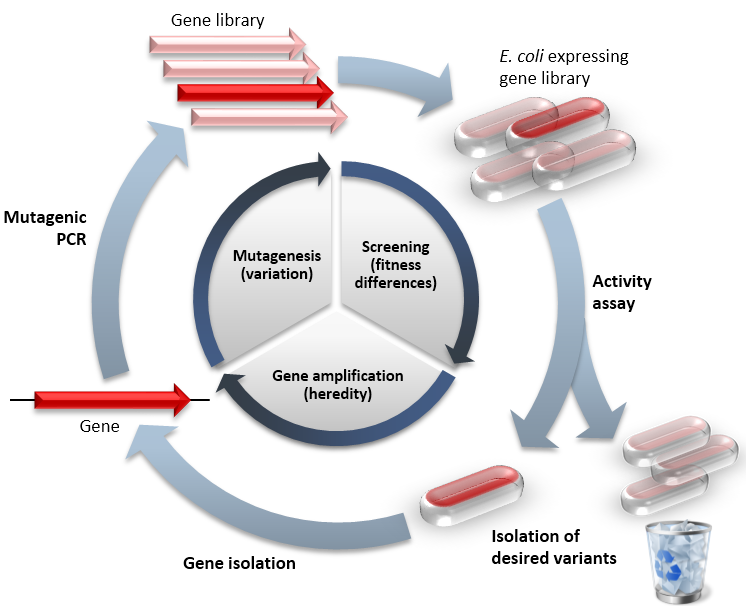
\includegraphics[scale=.6]{DEcycle.png}
	\caption{Esquema representativo de los pasos que contempla la evolución dirigida}
	\label{ed}
\end{figure}

El proceso, de manera general, consiste en someter un gen de interés a rondas iterativas de mutagénesis, con el fin de crear una biblioteca de variantes. A partir de dicho conjunto de elementos, se seleccionan las variantes con la función deseada. Finalmente, se aíslan y se amplifican para forman una plantilla para la siguiente iteración. Así el proceso sigue iterando y estadísticamente, se seleccionan las más favorables y aquellas que tendieron a la evolución debido a la supervivencia en el proceso \cite{arnold1998design}.

Con respecto al diseño racional de proteínas. Ésta, es una técnica ampliamente utilizada y al igual que la evolución dirigida, presenta el objetivo general de generar variantes con alguna función de interés o características particulares. No obstante, presenta una diferencia relevante, la cual se centra en la información que debe existir sobre la estructura, mecanismos, plegamiento o secuencia lineal de la proteína de interés \cite{carpenter1997rational}.

\section{Métodos computacionales aplicados en ingeniería de proteínas}

Diferentes métodos computacionales han sido desarrollados para distintos análisis, con el fin de poder de poder responder diferentes interrogantes planteadas desde enfoques distintos, ya sea, para estudiar secuencias lineales, filogenia y motivos conservados, análisis de estructuras, modelamiento, estudio de mutaciones, etc. A continuación, se listan algunos de los principales enfoques y qué herramientas existen para su desarrollo.

\subsection{Métodos de análisis filogenéticos} 

Los análisis filogenéticos se centran en el estudio de secuencias lineales de proteínas o genes, con el fin de identificar parentesco, motivos conservados o identificación de dominios. Las principales metodologías se basan en realizar alineamientos de secuencia con el fin de identificar o reconocer identidades de la secuencia estudio con respecto a información reportada previamente. 

Una de las herramientas más conocidas para el desarrollo de alineamientos es Blast \cite{kent2002blat}, el cual permite hacer múltiples comparaciones de secuencias versus bases de datos con genes o proteínas, empleando algoritmos de alineamiento local \cite{altschul1990basic}. 

Por otro lado, se encuentran los alineamientos múltiples, los cuales son utilizados en la comparación de secuencias lineales con el fin de encontrar patrones o motivos conservados, o, la identificación de parentesco \cite{Thompson1997}. Esto último, es muy utilizado cuando se analizan secuencias de organismos no secuenciados y cuya función se trata de aclarar. Una de las herramientas más utilizadas en esta área es el software Mega \cite{mst197}.

A su vez, el uso de los conceptos filogenéticos, ha sido utilizado para el estudio de propensiones de sustituciones aminoacídicas y cómo éstas afectan a la función de la proteína o con respecto a sus propiedades fisicoquímicas. Considerando esto, herramientas como MOSST \cite{Olivera-Nappa2011}, han permitido comprender la propensión de residuos y posiciones relevantes en secuencias, sólo estudiando conjuntos de elementos sin la necesidad de conocer estructuras tridimensionales de las proteínas.

Estos estudios, generan las bases para el análisis de secuencias y se basan en que sólo se necesita la secuencia lineal a estudiar y a partir de ella, es factible comprender un panorama relacionado a patrones de conservación, tendencias, relaciones evolutivas o inclusive, propensiones y posiciones relevantes. No obstante, no son los únicos, ya que existen herramientas computacionales que facilitan la predicción de la estructura secundaria, funcionalidad, etc., siendo una de las principales herramientas Swiss-Prot \cite{boeckmann2003swiss}.

\subsection{Métodos de análisis de estructuras}

Los métodos de análisis de estructuras, tienen el objetivo de comprender patrones de interacción, efectos de energía y estudiar diferentes propiedades fisicoquímicas y termodinámicas, a partir de la estructura tridimensional de una proteína, la cual puede ser obtenida por cristalografía de rayos X o por medio de resonancia magnética nuclear.

No obstante, también, es factible el desarrollo de modelos de proteínas a partir de secuencias lineales, técnica conocida como Modelamiento por homología. Diferentes software, permiten la implementación de esta técnica, dentro de los cuales se encuentran SWISS-MODEL \cite{Guex1997}, IntFOLD \cite{mcguffin2015intfold}, ROSETTA \cite{leaver2011rosetta3}, MODELLER \cite{eswar2006comparative}, entre los principales. 

Por otro lado, existen diferentes métodos computacionales que permiten el estudio de interacción entre proteína y una molécula o proteína-proteína, los cuales, principalmente se enfocan en el uso de técnicas como docking o dinámicas moleculares, con el fin de estudiar los posibles residuos que participan en la interacción, evaluándose a nivel energético y midiendo el desempeño en términos de error. A su vez, técnicas basadas en simulaciones moleculares, permiten comprender la interacción en sí, y, simular el comportamiento entre la molécula de interés y la proteína. Además, métodos computacionales basados en la química cuántica, han sido utilizados para comprender fenómenos de interacción a una escala mucho más precisa. No obstante, estos, son ampliamente más costosos y su uso es limitado al estudio de un número pequeño de átomos. 

Existen diferentes herramientas que permiten hacer dinámicas moleculares, tales como: NAMD \cite{phillips2005scalable}, AMBER \cite{case2005amber}. etc., mientras que para la interacción entre moléculas, o docking, existen AutoDock \cite{trott2010autodock}, RosettaDock \cite{lyskov2008rosettadock}, GRAMM-X \cite{tovchigrechko2006gramm}. Además de la suite Maestro Shr\"odinger \cite{release20161}, la cual abarca funcionalidades para las diferentes acciones propuestas. 

Distintos son los enfoques pueden ser considerados en el estudio de proteínas y en el análisis de su estructura. Sin embargo, los nombrados son los principales.
 
\subsection{Métodos de estudio de mutaciones}

De modo general, los estudios de mutaciones se basan principalmente en el análisis de la estructura ante los cambios de residuos o la adición o eliminación de estos, evaluando los cambios mediante diferencias de energía libre, entre la proteína inicial y la mutada. Herramientas como FoldX \cite{Schymkowitz2005}, SDM \cite{Pandurangan2017}, Auto-Mute \cite{Masso2010}, etc., permiten analizar cómo afecta una mutación en términos energéticos, basándose para ello, en el uso de funciones de energía potencial y dinámicas moleculares asociadas a dicha sustitución. Sin embargo, el uso de este tipo de herramientas, conlleva un gran costo computacional debido a los diferentes cálculos que son requeridos. Durante el capítulo \ref{cap2} se ahondarán más en estas herramientas. No obstante, en la Tabla \ref{tab:tab-summary-tools} se resumen algunas de las principales herramientas utilizadas para este tipo de análisis.

\subsection{Métodos basados en minería de datos y aprendizaje supervisado}

La minería de datos y el aprendizaje de máquinas, han sido utilizados en diferentes áreas del estudio de proteínas, ya sea para predicción de estructura secundaria \cite{hua2001novel, Muggleton1992, WANG2008262}, análisis del efecto de mutaciones \cite{capriotti2005mutant2, capriotti2008three, vaisman}, identificador de patrones mediante métodos de clustering \cite{schueler2003conserved, orengo1997cath}, entre los principales ejemplos.

Diferentes enfoques han sido aplicados para obtener resultados relevantes, por un lado, se encuentra la utilización de algoritmos de aprendizaje supervisados clásicos como métodos de clasificación o predicción. por otro, el uso de métodos de clustering para identificación de patrones basados en entornos no supervisados. Actualmente, se ha empleado el uso de redes neuronales y deep learning para manipulación de sistemas de datos complejos y se han enfocado principalmente en el estudio de predicción de interacciones y evaluación de estructura secundaria de una secuencia lineal.

A pesar de los diferentes objetivos, es necesario el desarrollo de conjuntos de datos que sean descritos mediante atributos, los cuales permitan alimentar estos modelos, para generar el aprendizaje. Distintas técnicas han sido utilizadas para caracterizar los ejemplos. dentro de las cuales, principalmente se encuentran la codificación mediante One hot encoder \cite{pedregosa2011scikit}, el uso de frecuencias de residuos \cite{ozbudak2014protein} y la descripción empleando propiedades fisicoquímicas en conjunto con la caracterización del ambiente \cite{capriotti2005mutant2, capriotti2008three}.

Actualmente, la minería de datos y el aprendizaje automático, son una de las áreas de desarrollo de mayor interés, ya que, generan una disminución en cuanto al tiempo de cómputo y maximiza los espacios de búsqueda, los cuales, por medio de técnicas experimentales, es muy complejo analizarlas y empleando métodos computacionales para evaluar las interacciones, demandan un alto costo computacional.

Otro tipo de enfoque, se basan en el modelamiento matemático de proteínas, empleando estructuras de grafos \cite{canutescu2003graph, vishveshwara2002protein}, con el fin de aprovechar las características y ventajas que entrega este análisis, para poder descubrir patrones o estudiar interacciones por medio de la formación de aristas entre los diferentes nodos \cite{martin2017loto}.

Enfoques particulares se han desarrollado con el fin estudiar estructuras específicas o regiones de interés, ejemplos como la identificación de epítopes en secuencias lineales de antígenos, son una de las problemáticas más relevantes y de mayor impacto en los últimos años \cite{jespersen2017bepipred, odorico2003bepitope, saha2008abcpred}. Sin embargo, la complejidad es alta, dada, la basta cantidad de información existente y a que las regiones con las que pueden interactuar, presentan un espacio muestral del orden del $10^9$.

Los resultados satisfactorios obtenidos mediante la aplicación de técnicas de minería de datos y aprendizaje de máquinas, demuestran el poder de éstas en las diferentes áreas de estudio asociadas a la ingeniería de proteínas, convirtiéndola en una de las temáticas de mayor impacto en el último tiempo. Inclusive, permite ser un complemento relevante para investigaciones de alto impacto, tal es el caso de investigadores como Frances H. Arnold, quien en el último tiempo, ha enfocado su análisis de evoluciones dirigidas hacia un enfoque de aprendizaje de máquinas, empleando diferentes técnicas asociadas al reconocimiento de patrones y la clasificación de estos \cite{bedbrook2019machine, wu2019machine, yang2018machine}.

\section{Minería de datos}


Minería de datos es el proceso de descubrimiento de patrones en set de datos, involucrando métodos asociados a Machine Learning \cite{michie1994machine}, estadísticas y sistemas de bases de datos \cite{hand2006data}. Se define como un subcampo interdisciplinario de la informática, el cual tiene por objetivo general extraer información (a través de métodos inteligentes) de un conjunto de datos y transformar la información en una estructura comprensible para su uso posterior \cite{fayyad1996knowledge, dunham2006data}. 

La minería de datos es el paso de análisis del proceso de \textit{descubrimiento de conocimiento en bases de datos}, o KDD \cite{fayyad1996kdd}. Además del análisis en bruto de los datos, también incluye aspectos de manipulación de bases de datos y pre procesamiento de estos, evaluaciones de modelo e inferencia, métricas de interés, consideraciones de complejidad, post procesamiento de estructuras descubiertas, visualización y actualización de la información \cite{berry2004data}.

En la Figura \ref{intro1}, se exponen las principales ramas que componen la minería de datos y los diferentes procesos que se asocian a dichas ramas.

\begin{figure}[!h]
	
	\centering
	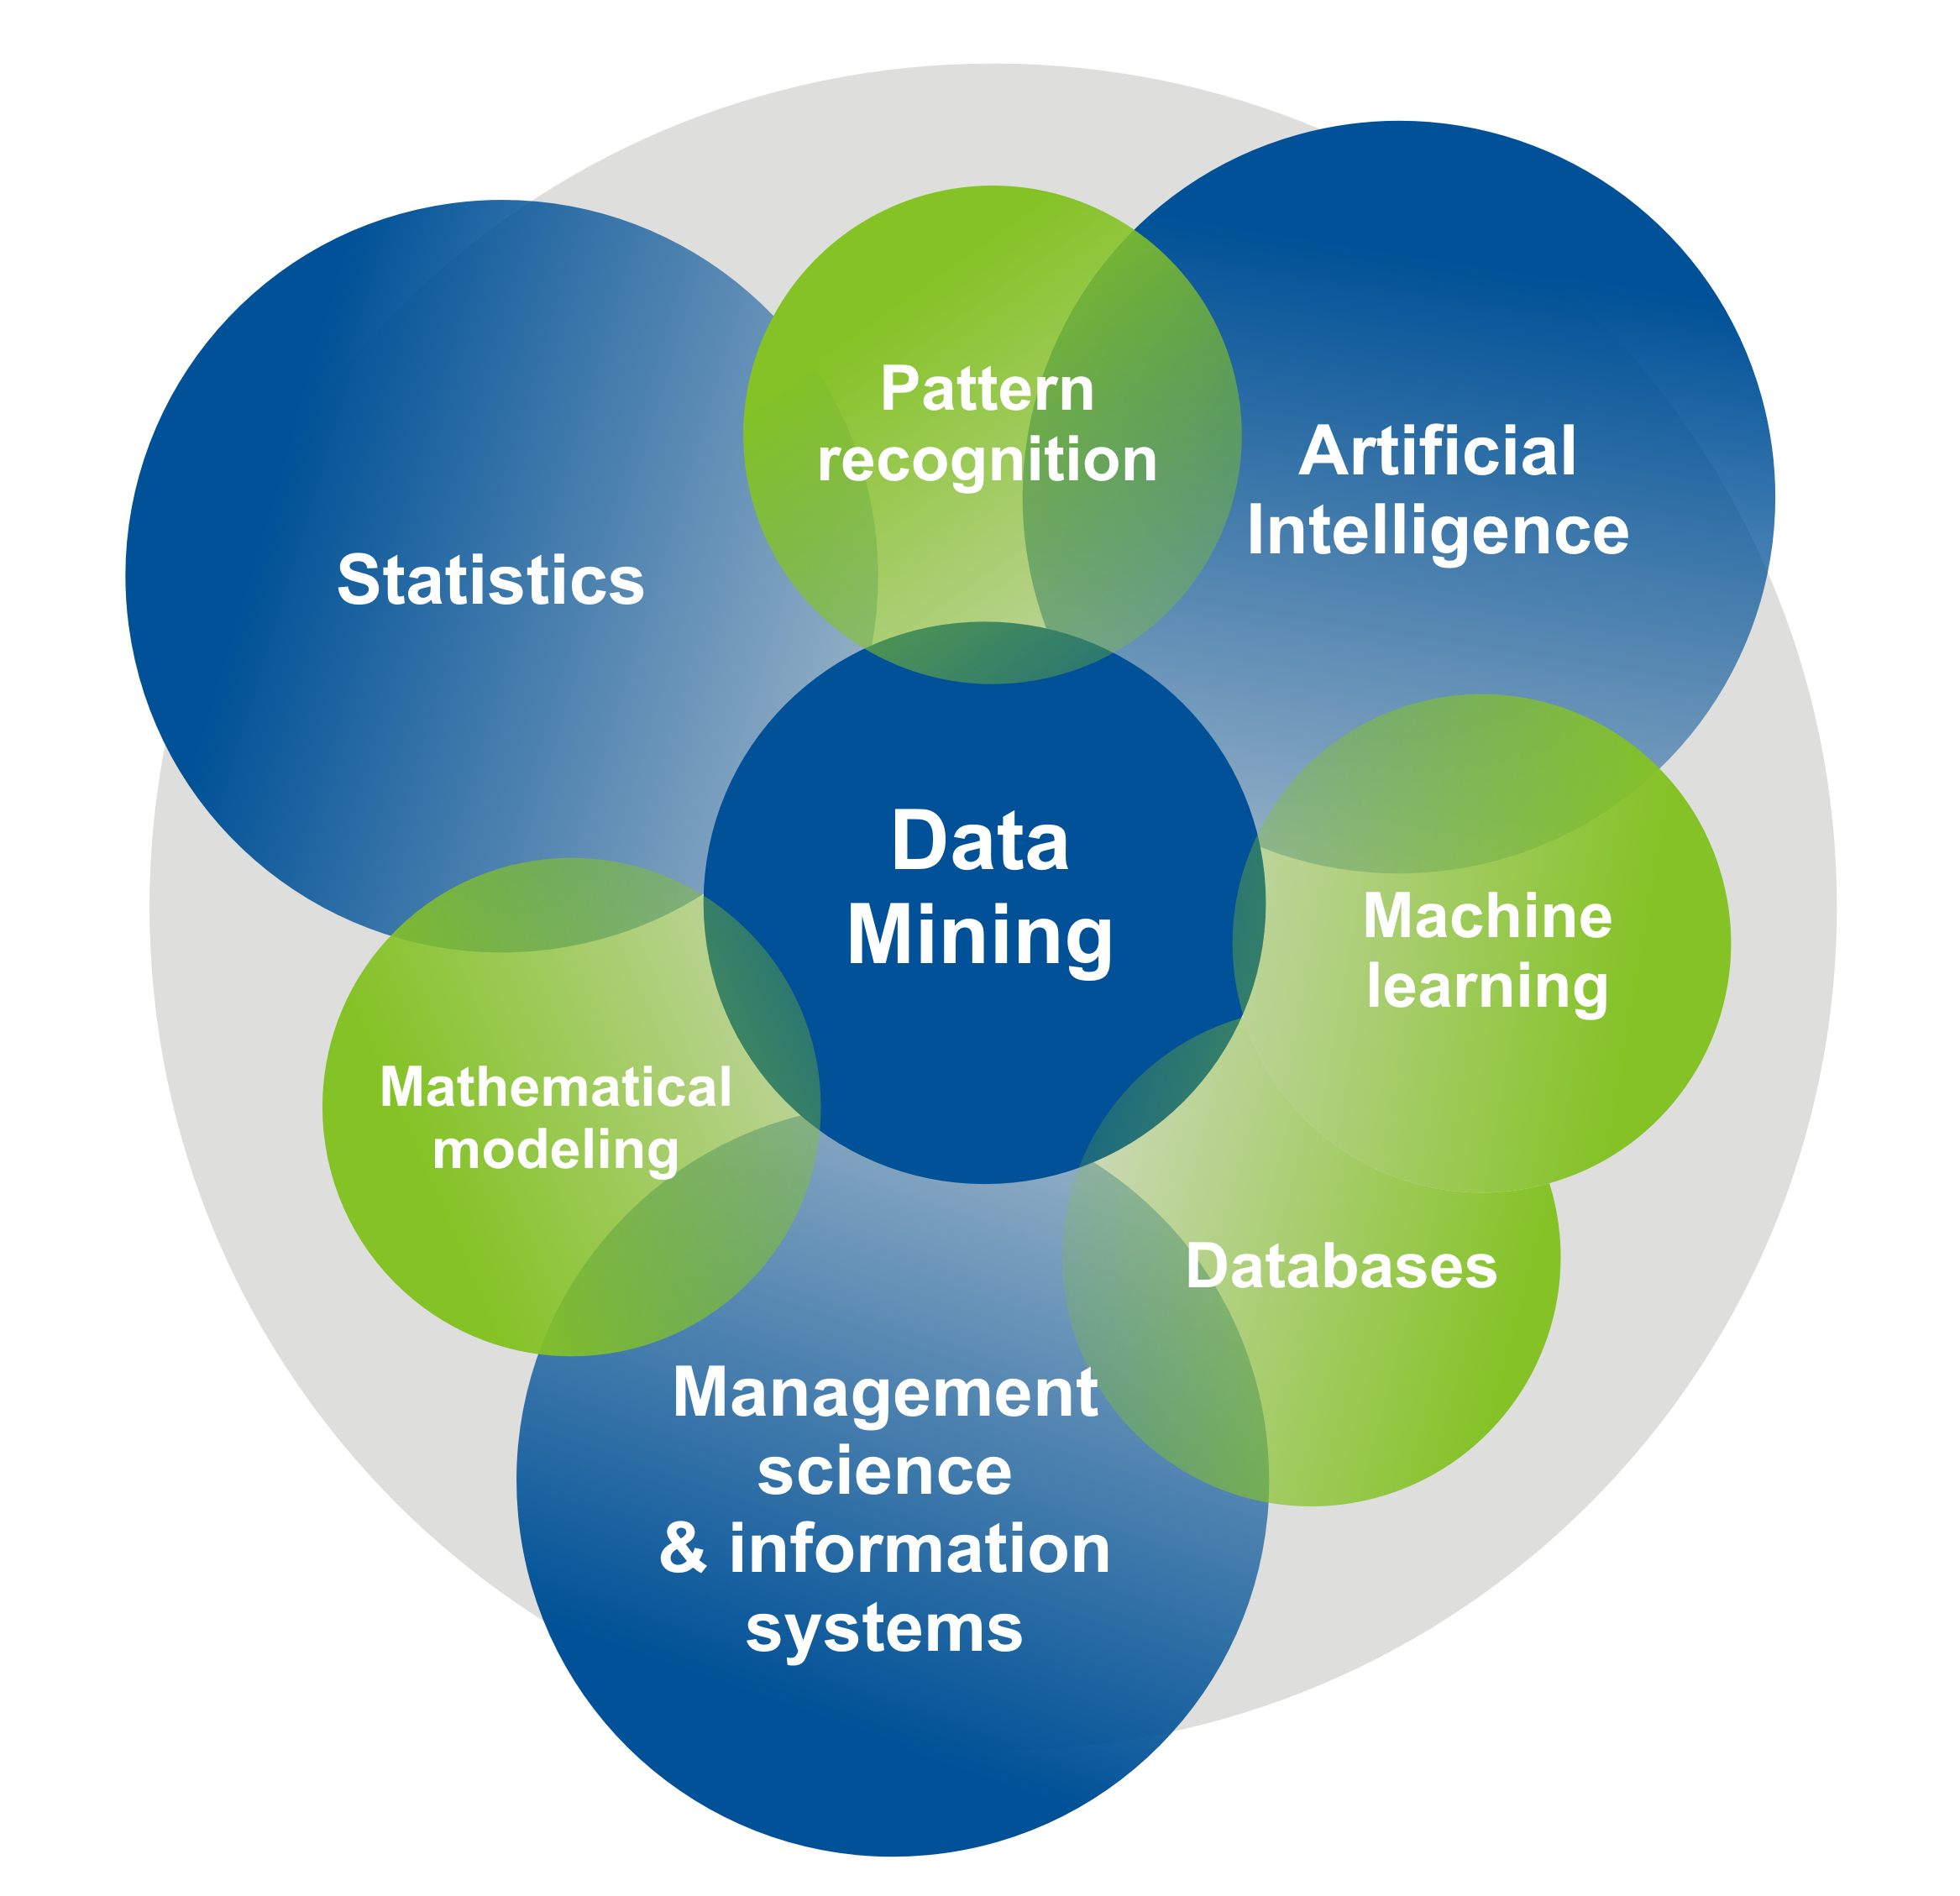
\includegraphics[scale=.4]{dataMining.jpg}
	\caption{Componentes principales de la minería de datos}
	\label{intro1}
\end{figure}

Son tres las principales áreas que abarca la minería de datos: Estadística, Inteligencia Artificial y Manipulación de sistemas de información. Por otro lado, son distintos procesos los que interactúan entre estas ramas, tales como: Modelamiento Matemático, reconocimiento de patrones, Sistemas de almacenamiento persistente y machine learning \cite{hand2006data}.

Cada área en particular, tiene un objetivo general y diversos objetivos específicos. Sin embargo, estas áreas interactúan entre sí, con el fin de poder extraer patrones de información que generen conocimientos a partir de la data de procesada \cite{berry2004data}.

La minería de datos se utiliza en diferentes campos, tales como: genética y genómica \cite{Lee2008, Rebhan1998}, ingeniería de proteínas \cite{han2009research, 4548625, li2008fast}, comercio y negocios \cite{hofmann2013rapidminer}, sistemas de tránsito \cite{Ma2013}, optimizaciones en procesos industriales \cite{Chien2008, 8051033, 983448}, reconocimiento de patrones \cite{jain1988algorithms, fayyad1996data}, rasgos cuantificables en enfermedades \cite{Yoo2012, obenshain2004, LDuan} y más recientemente en áreas de dinámicas moleculares \cite{Chen2017, Yang:2005:GFM:1081870.1081962} y parámetros para la generación de pipe lines automatizados de simulaciones cuánticas en sistemas químicos \cite{MAO2004787, PhysRevLett.91.135503, Ramakrishnan2015}.


\section{Principales problemáticas en la ingeniería de datos}

Diferentes son las problemáticas que pueden existir en el campo de la ingeniería de proteínas, ya sea, desde la generación de herramientas computacionales para estudiar mutaciones y su efecto de manera masiva, hasta diseño de mutaciones basados en secuencias lineales de proteínas. A continuación se presentan diferentes problemáticas existentes en el área, algunas de las cuales serán motivos de estudio y desafíos a cumplir durante el presente trabajo.

\subsection{Diferentes respuestas, una misma solución}

El desarrollo de modelos de clasificación y/o regresión, es uno de los temas más recurrentes en el campo de la minería de datos y el aprendizaje de máquinas. Sin embargo, el hecho de asociar mutaciones a una respuesta, conlleva al problema de cómo caracterizarla, con el fin de alimentar a los algoritmos para ser entrenados. 

A raíz de esto, cuáles son los mejores descriptores para una mutación?, desde qué puntos de vista se puede hacer una caracterización? y cuáles son más relevantes?, son interrogantes que se presentan a la hora de abordar su representación, siendo problemas que han sido tratados desde un largo tiempo, sin lograr generar un consenso o una forma general de diseñar tal representación. 

En un gran número de trabajos, en los cuales se ha evaluado la estabilidad de proteínas en torno a la mutación, se han utilizado descriptores termodinámicos y de ambiente para poder representar el elemento \cite{capriotti2005mutant2, capriotti2008three}. A pesar de que los desempeños de los estimadores han sido aceptables y relativamente altos. Esta caracterización ¿podrá ser utilizada para mutaciones asociadas a riesgo clínico?, ¿Existirá una correlación entre la respuesta y las variables de interés?, ¿Cómo afecta al desempeño del modelo la existencia de diferentes ejemplos asociados a distintas proteínas en un único conjunto de datos?, etc., son interrogantes que nacen a la hora de plantearse la situación.

Dado a lo anterior, y con el objetivo de generar un aporte significativo al desarrollo de estimadores basados en aprendizaje de máquinas, se ha propuesto adicionar el concepto de filogenia a la descripción de mutaciones y disgregar los conjuntos de elementos para ser tratados por proteínas independientes, esto con el fin de generar modelos de clasificación y/o regresión proteína-específicos, los cuales puedan ser aplicados a diferentes respuestas de interés ya sea: efectos en mutaciones, estabilidad, actividad, productividad, etc., siendo éste, el tema central a abordar en el capítulo \ref{cap2}.
 
\subsection{Codificaciones, cuáles es la mejor alternativa?}

A menudo, el uso de secuencias lineales de proteínas se relaciona a la identificación de patrones o evaluación de variantes para una misma proteína. Actuales herramientas bioinformáticas permiten el uso de la secuencia de manera directa y por medio de alineamientos de secuencias o modelamiento a través del uso de Cadenas de Markov facilitan el reconocimiento de patrones o la evaluación de mutaciones. No obstante, para la aplicación de métodos basados en minería de datos, ya sea la identificación de clusters o el entrenamiento de modelos, se requiere codificar la secuencia.

Existen diferentes codificaciones posibles, ya sea, para representar la secuencia o para la caracterización de mutaciones. A pesar de ello, no existe un consenso asociado a qué técnica utilizar. Cada una presenta sus pros y contra. No obstante, la cantidad de información involucrada varía entre ellas. Sin embargo, a mayor información, incrementa el número de dimensiones a tratar, aumentando la complejidad del problema. Esto implica, utilizar técnicas de reducción de dimensionalidad para seleccionar las dimensiones con mayor variabilidad en el conjunto de datos.

Una de las codificaciones más novedosas ha sido el uso de las propiedades fisicoquímicas de los residuos y su digitalización mediante transformadas de Fourier. Esto ha permitido la identificación de residuos claves en la propiedad en estudio y soluciona el problema del efecto del ambiente de los elementos participantes.

En vista de las necesidades de desarrollo de modelos de clasificación/regresión o la identificación de residuos claves y la generación de sistemas de clustering para secuencias lineales de proteína, con el fin de apoyar al diseño de mutaciones, análisis de variantes e inclusive caracterización de secuencias, sin tener conocimiento sobre su estructura. Se propone el uso de transformadas de Fourier como método de digitalización de propiedades fisicoquímicas para el desarrollo de conjuntos de datos que permitan ser entrenados para el desarrollo de estimadores o identificar patrones, siendo el tema central a abordar en el capítulo \ref{cap3}.

\subsection{Diseñar mutaciones, un arte poco apreciado}

Diseñar mutaciones de manera eficiente, con una identificación adecuada de la propiedad en estudio o funcionalidad a adicionar, sin incurrir en grandes costos económicos y de recursos, es uno de los \textit{Santos griales} de la ingeniería de proteínas. Como se nombró previamente, son dos enfoques los que utilizan actualmente: Evolución dirigida y diseño racional de proteínas.

Ambas técnicas tienen sus ventajas y desventajas. No obstante, poseen en común una demanda en tiempo elevada y se requiere de conocimientos elevados sobre la estructura para poder diseñar las mutaciones, al menos, para el caso de diseño racional. 

Enfoques computacionales han sido propuestos, con el fin de minimizar los costos económicos, contemplando evaluaciones energéticas asociadas a los residuos y cómo estos afectan a la estabilidad. No obstante, no pueden ser utilizados en secuencias lineales. Además, dejan de lado el concepto filogenético en el estudio, resultado un gap entre ambos puntos de vista. Por otro lado, métodos basados en la minería de datos, sólo se han centrado en identificación de residuos o el entrenamiento de modelos para predecir estabilidad.

A partir de lo anterior, y con el fin de generar un aporte significativo en el área de diseño, se ha considerado esta problemática como un foco central y culminante para el desarrollo de este trabajo de título, proponiendo así, la implementación de una herramienta computacional, basada en técnicas de minería de datos y aprendizaje de máquinas, que permita proponer mutaciones a un conjunto de variantes con respuesta conocida. Generando la codificación de la secuencia por medio del uso de propiedades fisicoquímicas y su respectiva digitalización a través de transformadas de Fourier, seleccionando las propiedades más relevantes por medio de la aplicación de técnicas de reducción de dimensionalidad, para así, entrenar modelos de clasificación o regresión y posterior a ello, proponer mutaciones enfocadas en un filtro, aplicando herramientas de análisis de estabilidad y propensión. Toda esta problemática, el planteamiento de la metodología y qué se utilizará para llevar a cabo, se abordará en el capítulo \ref{cap4}.


\subsection{Los descartados tienen algo más que decir}

En la técnica de evolución dirigida, la selección de residuos o variantes, se basa en si presentan la característica deseable o no, o si aumenta la propiedad. Si el residuo no provoca el efecto deseado, éste es descartado, ya que no cumple con el criterio de selección.

Sin embargo, es posible pensar que, combinaciones lineales de residuos pueden provocar una sinergia en alguna propiedad, generando el resultado deseado. No obstante, el estudio de dichas combinaciones, o mejor dicho, las correlaciones asociativas existentes entre mutaciones no son consideradas, ya que, sólo se seleccionan aquellos que cumplen con dicho criterio. Pero, ¿qué pasa con aquellos residuos que son descartados y que al ser mutados al mismo tiempo con otro elemento provocan el efecto deseado, e inclusive, con mejores resultados que los brindados por los seleccionados?, ¿Existe información asociada a conjuntos de mutaciones que provoquen este efecto?, ¿Será posible idear una metodología \textit{in-silico} que permita comprender este tipo correlaciones y justificar los resultados esperados?.

Como se puede comprender, este fenómeno no ha sido explotado desde el punto de vista de minería de datos, debido principalmente, a que no existen reportes de conjuntos de datos con dichas características y esto es debido a que no ha sido un foco de estudio central. Sin embargo, se cree que es una necesidad inminente, la comprensión de estos mecanismos, ya que, aumenta el espacio de búsqueda y posterior diseño de mutaciones, en un gran número de dimensiones. Además, si bien, resultados de este estilo no han sido reportados, si, a partir de experiencias de diferentes grupos con enfoque en diseño de mutaciones y evolución dirigida, han observado que residuos no seleccionables por si solos, en combinación con otro elemento, permiten obtener la característica deseable.

A pesar de que esta problemática, no se considera dentro de los temas de estudio en sí, se plantea la discusión y se propone como un problema a ser tratado en el corto plazo, debido a las grandes implicatorias que esto puede conllevar y a las expectativas que se pueden generar al respecto, siendo de utilidad a la hora de proponer nuevas mutaciones y generar un aporte significativo en el área de ingeniería de proteínas.
 
\section{Hipótesis}

En base a las herramientas computacionales existentes y a los problemas expuestos previamente, además, tomando en consideración los avances en minería de datos y aprendizaje de máquinas. Se propone la siguiente hipótesis.

\begin{center}
	\textit{Es factible el uso de técnicas de minería de datos y reconocimiento de patrones para el estudio y diseño de mutaciones in-silico?, considerando tanto desarrollo de modelos de evaluación cómo herramientas computacionales que permitan proponer variantes dada la información existente.}
\end{center}

Se plantea una hipótesis general, la cual abarca los diferentes o considera los planteamientos de problemáticas expuestos. Además, se menciona que la estructura de este proyecto es un conjunto de metodologías independientes. Es decir, cada capítulo en sí (2, 3 y 4) son herramientas computacionales independientes y tratan de resolver una problemática de las planteadas, por lo que, cada uno presenta en sí, su hipótesis y objetivos correspondientes. No obstante, a pesar de su independencia, tienen relación profunda con el abordaje de las soluciones a partir de técnicas de minería de datos, además, que es posible combinarlas, para desarrollar una suite de librerías de apoyo a la ingeniería de proteínas.

\section{Objetivos}

Continuando con la lógica expuesta previamente, es decir, cada uno de los siguientes capítulos resuelve una de las problemáticas planteadas, y contempla en sí, una herramienta computacional por sí sola. Se plantea a continuación el objetivo general.

\subsection{Objetivo general}

Diseñar e implementar suite de herramienta computacional basada en técnicas de minería de datos, aprendizaje de máquinas y reconocimiento de patrones, enfocada en el estudio de mutaciones, que permita ser un aporte sustancial en el campo de ingeniería de proteínas.

\subsection{Objetivos específicos}

Como se expuso previamente, cada siguiente capítulo corresponde a una herramienta en sí, que formará parte de esta gran suite computacional de apoyo al estudio de mutaciones \textit{in-silico}. Dado esto, se plantean los siguientes objetivos específicos.

\begin{enumerate}
	
	\item Diseñar, implementar y testear, herramienta computacional, inspirada en la estrategia de Meta-learning, para la evaluación de mutaciones puntuales el proteínas específicas, considerando como descriptores, propiedades termodinámicas, estructurales y conceptos filogenéticos. 
	
	\item Modelar, implementar y evaluar, herramienta computacional para la codificación de secuencias lineales de proteínas, empleando digitalización de propiedades fisicoquímicas, por medio de transformadas de Fourier, la cual permita la identificación de residuos claves y la aplicación de algoritmos de aprendizaje supervisado y clustering, para el entrenamiento de modelos y el reconocimiento de patrones.
	
	\item Diseñar, implementar y testear, herramienta computacional para el diseño de mutaciones \textit{in-silico}, basadas en técnicas de minería de datos y reconocimiento de patrones, enfocadas en secuencias lineales y modelos de aprendizaje supervisado, cuyos descriptores sean espectros de frecuencia basados en transformadas de Fourier y se constituya por herramientas de filtro, que aseguren estabilidad a la proteína y propensión al cambio en base a conceptos filogenéticos.
	
\end{enumerate}

Tal como se puede observar, los aprendizajes y competencias adquiridas al cumplir el objetivo 1 y 2, se utilizan en el desarrollo del objetivo 3. Lo cual denota una especie de dependencia entre las metodologías a plantear. Sin embargo, cada uno de los objetivos, corresponde a una herramienta computacional independiente, la cual podrá ser utilizada para los fines que el usuario estime conveniente. El conjunto de éstas, se asocia al desarrollo de la suite computacional de estudio de mutaciones empleando técnicas de minería de datos, reconocimiento de patrones y aprendizaje de máquinas.

Cada uno de los siguientes capítulos, presenta su propio marco teórico, además de hipótesis y objetivos, asociados a una metodología que trata de cumplirlos. No obstante, todos enfocados en un mismo punto: desarrollo de herramientas de apoyo para el estudio de mutaciones.
%!TEX root = ../thesis.tex
%*******************************************************************************
%****************************** Second Chapter *********************************
%*******************************************************************************

\chapter{Modelos predictivos asociados a mutaciones puntuales en proteínas \label{cap2}}

\ifpdf
    \graphicspath{{Chapter2/Figs/Raster/}{Chapter2/Figs/PDF/}{Chapter2/Figs/}}
\else
    \graphicspath{{Chapter2/Figs/Vector/}{Chapter2/Figs/}}
\fi

El análisis del efecto de mutaciones puntuales en proteínas, es una de las problemáticas más estudiadas en los últimos años. Las investigaciones se enfocan principalmente, en la evaluación de cambios en la estabilidad de la proteína mediante la variación de energía libre que la mutación provoca \cite{Schymkowitz2005,Pandurangan2017,rohl2004protein,Parthiban2006}. 

Diferentes modelos predictivos han sido desarrollados para poder predecir cambios de energía libre, en base a algoritmos de aprendizaje supervisado o mediante técnicas de minería de datos, y así, determinar el efecto de la mutación en set de proteínas de interés \cite{Quan2016,Capriotti2008,Broom2017,Khan2010,vaisman,Getov2016,Capriotti2005}. No obstante, en casos más específicos, se han desarrollado modelos para proteínas independientes, con el fin de asociar la mutación a un rasgo clínico, particularmente, enfocado a casos de cáncer \cite{article, Forbes2010}, cambios en termo estabilidad \cite{Tian2010}, propiedades geométricas \cite{Barenboim2008}, entre las principales.

Sin importar el uso o la respuesta de los modelos, es necesario construir set de datos con ejemplos etiquetados, es decir, cuya respuesta sea conocida para poder entrenar modelos basados en algoritmos de aprendizaje supervisado y así evaluar su desempeño. Los enfoques principales al desarrollo de descriptores se basan en propiedades fisicoquímicas y termodinámicas, así como también, el ambiente bajo el cual se encuentra la mutación \cite{Capriotti2005}, ya sea a partir de la información estructural o sólo considerando la secuencia lineal. Sin embargo, no son considerados, los componentes asociados a conceptos filogenéticos y la propensión a cambios de dicha mutación generando un gap entre ambos puntos de vista \cite{Olivera-Nappa2011}.

Dado a los modelos existentes y en vista a la necesidad de generar nuevos sistemas de predicción para mutaciones puntuales en proteínas, en respuesta al aumento considerable de reportes en los últimos años, se propone una nueva metodología para el diseño e implementación de modelos predictivos en mutaciones puntuales de proteínas.

Las mutaciones son descritas desde los puntos de vista estructural, termodinámico y filogenético. El desarrollo de los predictores es inspirado en el concepto de Meta Learning y es apoyado con técnicas estadísticas, tanto para la selección de modelos como para la evaluación de medidas de desempeño, entregando como resultado, un conjunto de modelos para las mutaciones puntuales reportadas, unificados en un único meta modelo.

Esta metodología será aplicada para generar estimadores en diferentes proteínas con mutaciones reportadas con respuesta conocida, como por ejemplo: evaluando las diferencias de energía libre que provoca la mutación y clasificaciones para evaluar si la sustitución de residuos aumenta o disminuye la estabilidad. A su vez, se implementarán modelos de clasificación para determinar la propensión clínica en un conjunto de mutaciones conocidas relacionados con el gen \textit{p}VHL, responsable de la enfermedad von Hippel Lindau, con el fin de exponer la versatilidad de la metodología y los problemas relevantes a set de datos altamente no-lineales.

A continuación, se describen los principales conceptos relacionados a aprendizaje supervisado, seguido de algunas herramientas computacionales para el análisis de mutaciones y su relevancia en la de estabilidad de una proteína, continuando con la metodología propuesta, la caracterización de los diferentes set de datos a utilizar y resultados parciales obtenidos al aplicar esta metodología.

\section{Aprendizaje de Máquinas}

Aprendizaje de Máquina, es una rama de la inteligencia artificial que tiene por objetivo el desarrollo de técnicas que permitan a los computadores aprender, es decir, generalizar comportamientos a partir de una información no estructurada suministrada en forma de ejemplos \cite{michie1994machine}. Aplicándose en diferentes campos de investigación: motores de búsqueda \cite{cooley1997web}, diagnósticos médicos \cite{7912315,ABDELAZIZ2018117}, detección de fraude en el uso de tarjetas de crédito, bioinformática \cite{juanito}, reconocimiento de patrones en imágenes \cite{imageA} y textos \cite{netzer2011reading,alm2005emotions}, etc. 

Los algoritmos de aprendizaje pueden clasificarse en dos grandes grupos \cite{michie1994machine}:

\begin{itemize}
	
	\item \textbf{Supervisados}: se cumple un rol de predicción, clasificación, asignación, etc. a un conjunto de elementos con características similares, por lo que los datos de entrada son conocidos.
	
	\item \textbf{No Supervisados}: su objetivo es agrupar en conjuntos con características similares los elementos de entrada dado los valores de estos atributos, en base a la asociación de patrones característicos que representen sus comportamientos.
\end{itemize}

A continuación se describen en forma general, los algoritmos de aprendizaje supervisados utilizados para el desarrollo de la metodología, explicando los conceptos bajo los que se basan y cómo estos entrenan y se emplean para predecir o clasificar nuevos ejemplos.

\subsection{Algoritmos de aprendizaje supervisado}

Existen diferentes algoritmos de aprendizaje supervisado, los cuales pueden ser asociados a la clasificación de un elemento o la predicción de valores, dependiendo el tipo de respuesta existente en el conjunto de datos a estudiar. En el caso de respuestas con distribución continua, se trabajan con algoritmos de regresión, mientras que si la respuesta es binaria o multiclase y es representada por variables categóricas, los algoritmos se basan en clasificadores \cite{michie1994machine}.

A su vez, también se pueden dividir con respecto a la forma en que se trata el problema, existiendo algoritmos basados en cálculos de distancia entre ejemplos (K-Vecinos Cercanos), otros que consideran transformaciones vectoriales y aplicaciones de funciones de kernel (Máquina Soporte de Vectores), así como también el uso de las características como entorno espacial de decisión (Árboles y métodos de ensamble) y aquellos que utilizan redes neuronales y trabajan en torno a cajas negras, o métodos basados en regresiones lineales, sólo aplicados a modelos predictivos de variables continuas.

Cada uno de estos algoritmos es descrito a continuación, enfocándose tanto en el componente matemático asociado, así como también en las ventajas y usos posibles que estos puedan tener, con respecto al conjunto de datos a trabajar.

\subsection{Métodos basados en regresiones lineales}

Regresión lineal, es uno de los métodos más simples en cuanto a predicción de variables continuas, además de uno de los más limitantes debido al sobreajuste que éste puede generar. No obstante, permite evaluar de manera simple y sencilla conjuntos de datos \cite{graybill1976theory}. 

Matemáticamente, se espera que el conjunto de respuesta sea el resultado de una combinación lineal de parámetros, es decir. Sea $\hat{y}$ el vector de predicciones, se tiene que:

\begin{center}
	$\hat{y}(w, x) = w_0 + w_1 x_1 + ... + w_p x_p$
\end{center}

Donde $w_0$ es el intercepto y $w = (w_1,\cdots, w_p)$ el vector de coeficientes.

Existente diferentes métodos de regresión lineal, los cuales cumplen con el mismo objetivo. Sin embargo, la forma en la que minimizan el error asociado a las diferencias entre los valores predichos y los observados.

A modo de ejemplo, en la Tabla \ref{tab:tab-regression} se exponen distintas formas de ajustar o minimizar el error asociado.

% Please add the following required packages to your document preamble:
% \usepackage{longtable}
% Note: It may be necessary to compile the document several times to get a multi-page table to line up properly
\begin{longtable}[c]{|l|l|l|}
	\hline
	\multicolumn{1}{|c|}{\textbf{\begin{tabular}[c]{@{}c@{}}Tipo de\\ regresión\end{tabular}}} & \multicolumn{1}{c|}{\textbf{Minimización}} & \multicolumn{1}{c|}{\textbf{Descripción}}                                                                                                                                   \\ \hline
	\endfirsthead
	%
	\endhead
	%
	\begin{tabular}[c]{@{}l@{}}Ordinary\\ Least\\ Squares \cite{golub1980analysis} \end{tabular}                         & $\min_{w} || X w - y||_2^2$                & \begin{tabular}[c]{@{}l@{}}Método más simple,\\ no implica parámetros\\ externos.\end{tabular}                                                                              \\ \hline
	\begin{tabular}[c]{@{}l@{}}Ridge\\ Regression \cite{hoerl1970ridge}\end{tabular}                                 &   $\min_{w} || X w - y||_2^2 + \alpha ||w||_2^2$                                         & \begin{tabular}[c]{@{}l@{}}Adición de penalización\\ $\alpha$.\end{tabular}                                                                                                 \\ \hline
	Lasso  \cite{hans2009bayesian}                                                                                    &  $\min_{w} { \frac{1}{2n_{\text{samples}}} ||X w - y||_2 ^ 2 + \alpha ||w||_1}$                                          & \begin{tabular}[c]{@{}l@{}}Reduce el número de\\ características bajo las\\ cuales depende la\\ solución final.\end{tabular}                                                \\ \hline
	Elastic-Net  \cite{zou2005regularization}                                                                              & $\min_{w} { \frac{1}{2n_{\text{samples}}} ||X w - y||_2 ^ 2 + \alpha \rho ||w||_1 +
		\frac{\alpha(1-\rho)}{2} ||w||_2 ^ 2} $                                           & \begin{tabular}[c]{@{}l@{}}Usado principalmente\\ en caso de atributos\\ con alta correlación.\end{tabular}                                                                 \\ \hline
	\begin{tabular}[c]{@{}l@{}}Orthogonal\\ Matching\\ Pursuit\\ (OMP) \cite{pati1993orthogonal}\end{tabular}            &   $\underset{\gamma}{\operatorname{arg\,min\,}}  ||y - X\gamma||_2^2 \text{ subject to } ||\gamma||_0 \leq n_{\text{nonzero\_coefs}}$                                         & \begin{tabular}[c]{@{}l@{}}Permite fijar el número\\ de coeficientes no nulos.\end{tabular}                                                                                 \\ \hline
	\begin{tabular}[c]{@{}l@{}}Bayesian\\ Regression \cite{castillo2015bayesian}\end{tabular}                              &  $p(y|X,w,\alpha) = \mathcal{N}(y|X w,\alpha)$                                          & \begin{tabular}[c]{@{}l@{}}Se adapta a de manera\\ eficiente a los datos de\\ entrenamiento y permite\\ incluir penalizaciones \\ asociadas a los coeficientes\end{tabular} \\ \hline
	\caption{Tipos de regresión con su función de minimización y descripciones correspondientes a las características que estos poseen.
	}
	\label{tab:tab-regression}\\
\end{longtable}

Pese a su simplicidad, los métodos basados en regresiones lineales han sido ampliamente utilizados. No obstante, presentan diferentes problemas asociados al sobreajuste de parámetros.
 
\subsection{K-Vecinos Cercanos}

Algoritmo de aprendizaje supervisado, el cual tiene por objetivo asociar un elemento a una clase en particular, dada la información de ejemplos de entrada que tengan asociadas características particulares, que puedan declararse como \textit{vecinos} del nuevo ejemplo a clasificar, siendo \textbf{k} el número de vecinos que se está dispuesto a utilizar para aplicar la clasificación \cite{6313426}. La mejor elección de \textbf{k} depende fundamentalmente de los datos; generalmente, valores grandes de \textbf{k} reducen el efecto de ruido en la clasificación, pero crean límites entre clases parecidas.

Con el fin de evaluar la cercanía de los ejemplos existentes contra el nuevo ejemplo a clasificar, es necesario asociar ciertas medidas de distancia que permitan cuantificar esta característica, para así poder comparar esta distancia y evaluar la cercanía para asociarle una clase a este nuevo ejemplo \cite{5408784}. La distancia a emplear para evaluar la cercanía puede ser: Euclidiana \cite{DANIELSSON1980227}, Manhattan \cite{PERLIBAKAS2004711}, coseno \cite{LIAO20155328} o Mahalanobis \cite{DEMAESSCHALCK20001}, entre las principales, las cuales son expuestas de manera general en la Tabla \ref{tab:tab-form-distance}.

% Please add the following required packages to your document preamble:
% \usepackage{longtable}
% Note: It may be necessary to compile the document several times to get a multi-page table to line up properly
\begin{longtable}[c]{|l|l|l|}
	\hline
	\multicolumn{1}{|c|}{\textbf{Distancia}} & \multicolumn{1}{c|}{\textbf{Fórmula}}                  & \multicolumn{1}{c|}{\textbf{Descripción}}                                                            \\ \hline
	\endfirsthead
	%
	\endhead
	%
	Euclideana                               & $D_{(X,Y)}\ =\ \sqrt{\sum_{i=1}^{l}(X_{i}-Y_{j})^{2}}$ & Se basa en una recta entre dos puntos                                                                \\ \hline
	Coseno                                   & $D_{(X,Y)}\ =\ \arccos(\frac{X^{T}Y}{||X||\ ||Y||})$   & \begin{tabular}[c]{@{}l@{}}Se basa en vectores y en el coseno del\\ ángulo que forman\end{tabular}   \\ \hline
	Manhattan                                & $D_{(X,Y)}\ =\ \sum_{i=1}{n} |X_{i}-Y_{i}|$            & Distancia en forma de zig-zag                                                                        \\ \hline
	Mahalanobis                              & $D_{(X,Y)}\ =\ \sqrt{(X-Y)^{T}S^{-1}(X-Y)}$            & \begin{tabular}[c]{@{}l@{}}Considera las correlaciones entre las\\ variables de estudio\end{tabular} \\ \hline
	\caption{Resumen tipos de distancias utilizadas en procesos de comparación de ejemplos
	}
	\label{tab:tab-form-distance}\\
\end{longtable}


K-Nearest Neighbors (KNN por su descripción en inglés), presenta algunos problemas, tales como: posibles errores al existir más de un elemento de distinta clase cercano al nuevo ejemplo a clasificar. Sin embargo, dicho error estimado es reducido \cite{6313426}.

Existen dos variaciones para la aplicación de KNN: aplicación basada en las distancias y aplicación basada en radios con respecto a puntos, la primera es mayormente usada. No obstante, en el caso de que los puntos no se encuentren uniformemente distribuidos es una mejor opción usar la segunda alternativa, siendo muy eficaz en problemas conocidos como \textit{la maldición de la dimensionalidad}\footnote{Para más detalles ver sección \ref{problemas}}. 

KNN utiliza el componente de peso \cite{TAN2005667}, es decir, valores asignados a puntos específicos para determinar si un elemento a clasificar es de una clase o no, normalmente se utilizan pesos uniformes. Sin embargo, es posible asignar valores de tal manera que al momento de realizar la votación puntos más cercanos en base a distancias presenten más peso que otros.

Se han implementando diversos algoritmos a la hora de aplicar la técnica de KNN, los cuales tienen relación con el coste computacional que presentan, dentro de estos se encuentran: Brute Force, K-D Tree y Ball Tree \cite{pedregosa2011scikit}.

Este algoritmo de aprendizaje supervisado, puede ser utilizado tanto para el entrenamiento de modelos de clasificación (respuestas categóricas) y de regresión (respuestas continuas).

\subsection{Naive Bayes}

Naive Bayes es un conjunto de algoritmos de aprendizaje supervisados basados en la aplicación del teorema de Bayes con la suposición "ingenua" de independencia entre cada par de características \cite{zhang2004optimality}. Dada una variable de clase $y$ y un vector de característica dependientes de la forma $x_1,..., x_n$, el teorema de Bayes establece la siguiente relación:

\begin{center}
	$P(y \mid x_1, \dots, x_n) = \frac{P(y) P(x_1, \dots x_n \mid y)} {P(x_1, \dots, x_n)}
	$
\end{center}

Utilizando la suposición ingenua de independencia de características, se tiene que:

\begin{center}
	$P(x_i | y, x_1, \dots, x_{i-1}, x_{i+1}, \dots, x_n) = P(x_i | y)$
\end{center}

Para todo $i$, esta relación se simplifica a:

\begin{center}
	$P(y \mid x_1, \dots, x_n) = \frac{P(y) \prod_{i=1}^{n} P(x_i \mid y)} {P(x_1, \dots, x_n)}$
\end{center}

Dado que $P(x_1, \dots, x_n)$ es constante dada la entrada, se puede utilizar la siguiente regla de clasificación:

\begin{center}
	$P(y \mid x_1, \dots, x_n) \propto P(y) \prod_{i=1}^{n} P(x_i \mid y)$
	
\end{center}

\begin{center}
	$\Downarrow$ 
\end{center}
\begin{center}
	$\hat{y} = \arg\max_y P(y) \prod_{i=1}^{n} P(x_i \mid y),$
\end{center}

A pesar de sus supuestos aparentemente simplificados, los clasificadores de Naive Bayes han funcionado bastante bien en muchas situaciones del mundo real, la famosa clasificación de documentos y el filtrado de spam son ejemplos de ello \cite{10.1007/BFb0026666, Chen2009, metsis2006spam}. Requieren una pequeña cantidad de datos de entrenamiento para estimar los parámetros necesarios. Pueden ser extremadamente rápido en comparación con métodos más sofisticados. El desacoplamiento de las distribuciones de las características condicionales de clase significa que cada distribución se puede estimar de forma independiente como una distribución unidimensional. Esto a su vez ayuda a aliviar los problemas derivados de la dimensionalidad. 

Existen distintos tipos de clasificadores de Naive Bayes, diferenciándose entre sí en la función de distribución de probabilidad que utilizan \cite{metsis2006spam,john1995estimating,manning2010introduction}, dentro de los que se encuentran:

\begin{itemize}
	
	\item \textbf{Gaussian Naive Bayes.}
	
	\begin{center}
		$P(x_i \mid y) = \frac{1}{\sqrt{2\pi\sigma^2_y}} \exp\left(-\frac{(x_i - \mu_y)^2}{2\sigma^2_y}\right)$
	\end{center}
	
	\item \textbf{Multinomial Naive Bayes.}
	
	La distribución se parametriza por el vector $\theta_y = (\theta_{y1},\ldots,\theta_{yn})$ para cada clase $y$, donde $n$ es el número de características y $\theta_{y1}$ es la probabilidad $P(x_i \mid y)$ de que la característica $i$ aparezca en una muestra que pertence a la clase $y$.
	
	Cada $\theta_y$ es estimado por:
	
	\begin{center}
		
		$\hat{\theta}_{yi} = \frac{ N_{yi} + \alpha}{N_y + \alpha n}$		
	\end{center}
	
	Donde $N_{yi} = \sum_{x \in T} x_i$ es el número  de veces que aparece la característica $i$ en la muestra de clase $y$ en el set de entrenamiento $T$ y $N_{y} = \sum_{i=1}^{|T|} N_{yi}$ representa el total de todas las características para la clase.
	
	\item \textbf{Bernoulli Naive Bayes.}
	
	\begin{center}
		$P(x_i \mid y) = P(i \mid y) x_i + (1 - P(i \mid y)) (1 - x_i)$
	\end{center}
	
\end{itemize}

\subsection{Árboles de Decisión}

Se define árbol de  decisión como un modelo de predicción, utilizado en el ámbito de la inteligencia artificial, en el cual,  dado un conjunto de datos, se fabrican diagramas de construcciones lógicas, muy similares a los sistemas de predicción basados en reglas, que sirven para representar y categorizar una serie de condiciones que ocurren de forma sucesiva, para la resolución de un problema.  

Aprendizaje basado en árboles de decisión es un método comúnmente utilizado en la minería de datos, cuyo objetivo consiste en desarrollar un modelo de predicción para el valor de una variable de destino en función de diversas variables de entrada \cite{freund1999alternating}.

El aprendizaje basado en árboles de decisión utiliza un árbol como un modelo predictivo que mapea las observaciones de las características que presenta un elemento. En estas estructuras de árbol, las hojas representan etiquetas de conjuntos ya clasificados, los nodos, a su vez, nombres o identificadores de los atributos y las ramas representan posibles valores para dichos atributos \cite{bhargava2013decision}.

A modo de ejemplo, se expone en la Figura \ref{arboles}, una representación de un posible árbol, el cual fue desarrollado para entrenar modelos de clasificación utilizando el set de datos iris \cite{fisher1936use}.

\begin{figure}[!h]
	
	\centering
	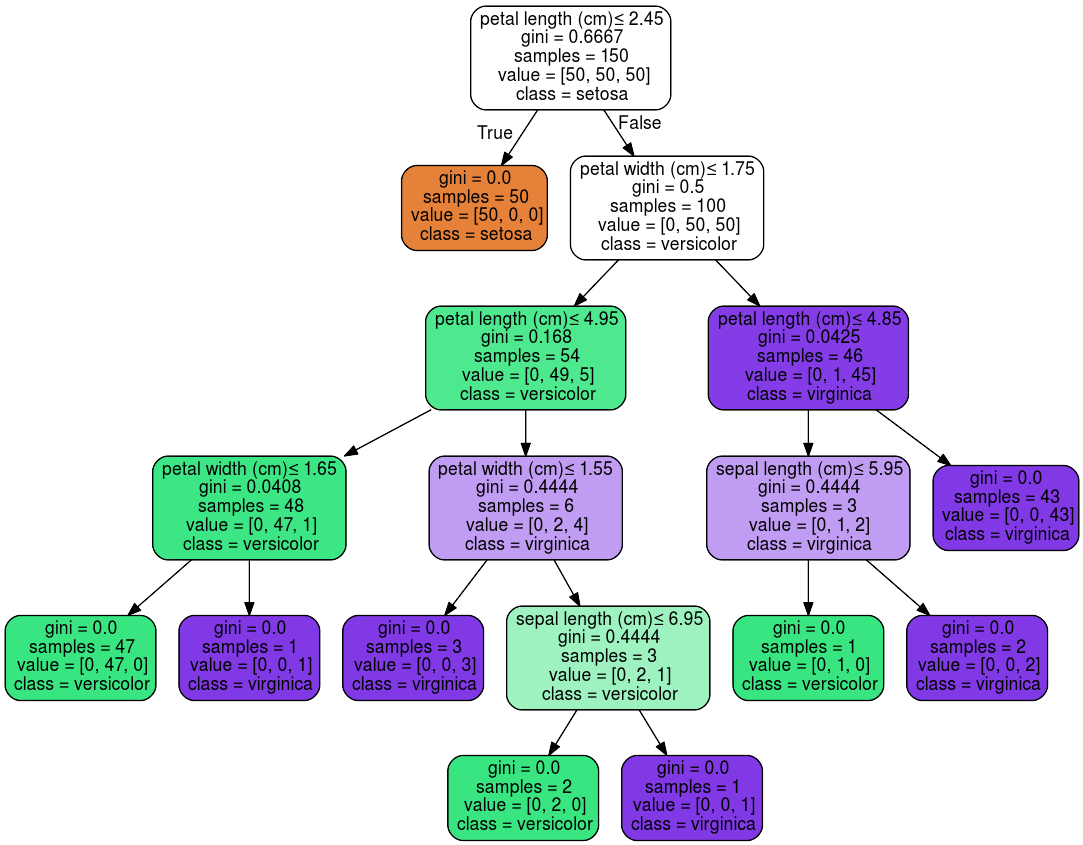
\includegraphics[scale=.4]{iris.png}
	\caption{Estructura de árbol para modelo de clasificación de set de datos iris.}
	\label{arboles}
\end{figure}


Un árbol puede ser entrenado mediante el fraccionamiento del conjunto inicial en subconjuntos basados en una prueba de valor de atributo. Este proceso se repite en cada subconjunto derivado de una manera recursiva, el cual es denominado \textit{particionamiento recursivo}. La recursividad termina cuando el subconjunto en un nodo $m$ tiene todos sus miembros el mismo valor de la variable categórica o pertenecen al mismo intervalo finito, para el caso en que las respuestas se asocian a distribuciones continuas, o cuando la partición ya no agrega valor a las predicciones.

Para cada división, es necesario el uso de una función que entregue una medida de impureza en cada partición, esto, con el objetivo de seleccionar el mejor subconjunto para un atributo dado, la elección de dicho descriptor, se basa en el objetivo de separar de mejor manera los ejemplos. 

La selección de los atributos se basa en qué atributo, al momento de clasificar, genera nodos más puros. Para ello, se utiliza una función de ganancia de información, la cual representa la ganancia  obtenida a partir de una división de los ejemplos de entrenamiento \cite{breiman2017classification}. 

Existen diferentes tipos de algoritmos bajo los cuales son implementados las ideologías de los árboles de decisión, cada uno presenta características particulares. Sin embargo, cumplen con el mismo objetivo. A modo general, en la Tabla \ref{tab:summary-alg-trees} se exponen algunos de los algoritmos existentes \cite{hssina2014comparative}.

% Please add the following required packages to your document preamble:
% \usepackage{longtable}
% Note: It may be necessary to compile the document several times to get a multi-page table to line up properly
\begin{longtable}[c]{|l|l|}
	\hline
	\multicolumn{2}{|c|}{\textbf{Algoritmos de árboles de decisión}} \\ \hline
	\endfirsthead
	%
	\endhead
	%
	\multicolumn{1}{|c|}{\textbf{Algoritmo}} & \multicolumn{1}{c|}{\textbf{Descripción}} \\ \hline
	Iterative Dichotomiser 3 (ID3) & \begin{tabular}[c]{@{}l@{}}Se crea un árbol de múltiples vías, encontrando para cada\\ nodo la característica categórica que producirá la mayor\\ ganancia de información. Por lo general, se aplica un\\ paso de poda para mejorar la capacidad del árbol asociada\\ a la generalización.\end{tabular} \\ \hline
	C4.5 & \begin{tabular}[c]{@{}l@{}}Permite manipular variables continuas, mediante la definición\\ dinámica de atributos discretos, dividiendo el valor continuo en\\ un conjunto finito de intervalos discretos. La poda se realiza\\ eliminando la condición previa de una regla si la precisión de\\ la regla mejora sin ella.\end{tabular} \\ \hline
	C5.0 & \begin{tabular}[c]{@{}l@{}}Genera un conjunto de reglas más pequeñas en comparación a\\ C4.5. Sin embargo, este último es más preciso en cuanto al \\ entrenamiento.\end{tabular} \\ \hline
	\begin{tabular}[c]{@{}l@{}}Classification and Regression\\ Trees (CART)\end{tabular} & \begin{tabular}[c]{@{}l@{}}Construye árboles binarios utilizando la característica y el\\ umbral que producen la mayor ganancia de información en\\ cada nodo.\end{tabular} \\ \hline
	\caption{Resumen de algoritmos comunes para la creación de árboles de decisión. }
	\label{tab:summary-alg-trees}\\
\end{longtable}

\subsubsection{Formulación matemática}

Una definición matemática, tanto del proceso de clasificación o regresión y cómo son los criterios de selección de atributos es expuesta a continuación.

Sea $x_{i} \in R^{n}$ los vectores de entrenamiento del conjunto de datos y sea $y \in R^l$ el vector de respuestas asociadas a cada ejemplo. Un árbol de decisión divide el espacio de forma recursiva, de manera que las muestras con las mismas etiquetas se agrupan.

Cada nodo $m$ puede ser representado por $Q$ y sea $\theta = (j, t_{m})$ la división candidata para un atributo $j$ y un umbral $t_{m}$, se definen las particiones $Q_{left}(\theta)$ y $Q_{rigth}(\theta)$ tal que:

\begin{align}
	\begin{aligned}
		Q_{left}(\theta) = {(x, y) | x_j <= t_m}\\Q_{right}(\theta) = Q \setminus Q_{left}(\theta)
	\end{aligned}
\end{align}
 

Asociado a las divisiones, se tiene que, cada nodo generado se mide con respecto a la impureza de éste, la cual, puede ser representada por una función $H()$ y a la ganancia de información que genera la división $G(Q, \theta)$, la cual se estima como:

\begin{center}
	$G(Q, \theta) = \frac{n_{left}}{N_m} H(Q_{left}(\theta))
+ \frac{n_{right}}{N_m} H(Q_{right}(\theta)$
\end{center}

Los descriptores se seleccionan con respecto a aquel que minimice la impureza de los nodos:

\begin{center}
	$\theta^* = \operatorname{argmin}_\theta  G(Q, \theta)$
\end{center}

Finalmente, se tiene que para los subconjuntos $Q_{left}(\theta^*)$ y $Q_{rigth}(\theta^*)$ la profundidad máxima se alcanza si:

\begin{itemize}
	
	\item $N_{m} < min_{samples}$ 
	
	\item $N_{m} = 1$
\end{itemize}

Con $N_{m}$ representando el número de nodos $m$.

Los criterios de clasificación se basan en la proporción de las clases según sus observaciones y en la función de impureza que es posible utilizar.

Si el vector de respuestas, es asociado a variables categóricas y toma valores entre $0,1,\cdots,k-1$ para un nodo $m$, representando una región $R_{m}$ con $N_{m}$ ejemplos, se tiene que la proporción  de observaciones de clase $k$ en un nodo $m$ puede definirse como:

\begin{center}
	$p_{mk} = 1/ N_m \sum_{x_i \in R_m} I(y_i = k)$
\end{center}

Con respecto a las diferentes funciones de impureza $H()$ que pueden ser utilizadas se tienen las siguientes, descritas en la Tabla \ref{tab:tab-form-impureza}. 

% Please add the following required packages to your document preamble:
% \usepackage{longtable}
% Note: It may be necessary to compile the document several times to get a multi-page table to line up properly
\begin{longtable}[c]{|l|l|}
	\hline
	\multicolumn{1}{|c|}{\textbf{Función}} & \multicolumn{1}{c|}{\textbf{Fórmula}}   \\ \hline
	\endfirsthead
	%
	\endhead
	%
	Gini                                   & $H(X_m) = \sum_k p_{mk} (1 - p_{mk})$   \\ \hline
	Entropía                               & $H(X_m) = - \sum_k p_{mk} \log(p_{mk})$ \\ \hline
	\textit{Misclassification}                      & $H(X_m) = 1 - \max(p_{mk})$             \\ \hline
	\caption{Tipos de medidas de impureza que pueden ser utilizadas en árboles de decisión para modelos de clasificación.
	}
	\label{tab:tab-form-impureza}\\
\end{longtable} 

Siendo $X_{m}$ datos de entrenamiento en el nodo $m$.

A la hora de entrenar modelos de regresión, es decir, con respuestas asociadas a una distribución continua, se tiene que para el nodo $m$, el cual representa una región $R_{m}$ con observaciones $N_{m}$, los criterios comunes para minimizar errores en futuras divisiones son el Error cuadrático medio y el Error absoluto medio, quienes minimizan el error tipo II y el error tipo I, respectivamente.

Estos se pueden definir como:

\begin{itemize}
	
	\item \textbf{Error cuadrático medio}: 
	
	\begin{align}\begin{aligned}\bar{y}_m = \frac{1}{N_m} \sum_{i \in N_m} y_i\\H(X_m) = \frac{1}{N_m} \sum_{i \in N_m} (y_i - \bar{y}_m)^2\end{aligned}\end{align}
	
	\item \textbf{Error absoluto medio}: 
	
	\begin{align}\begin{aligned}\bar{y}_m = \frac{1}{N_m} \sum_{i \in N_m} y_i\\H(X_m) = \frac{1}{N_m} \sum_{i \in N_m} |y_i - \bar{y}_m|\end{aligned}\end{align}
\end{itemize}

Este tipo de entrenamiento, es uno de los más utilizados, debido a su simplicidad a la forma en la que trabaja, ya que, permite comprender del problema, con respecto a los atributos y cómo estos van distribuyendo las respuestas, así, es posible entender las decisiones que toma el algoritmo para clasificar o predecir nuevos ejemplos, determinar comportamientos preferentes y tendencias sobre atributos y rangos de estos.

\subsection{Support Vector Machine (SVM)}

Máquina soporte de vectores (SVM por sus siglas en inglés), es un conjunto de métodos de aprendizaje supervisado, utilizados para clasificar, predecir e inclusive para la detección de puntos outliers  \cite{scholkopf2001learning}. 

SVM genera una representación de los ejemplos como puntos en el espacio, mapeados de modo que los ejemplos de las categorías separadas se dividan por un espacio claro que es tan amplio como sea posible. Nuevos ejemplos son entonces mapeados en ese mismo espacio y predicen si pertenecen a una categoría en base a qué lado del espacio son asignados \cite{scholkopf2001learning}.

Las predicciones se realizan de manera eficiente, utilizando funciones kernel para su transformación en espacios no lineales \cite{amari1999improving}. Esto permite generar transformaciones de espacio dimensional de los datos, para mapear implícitamente sus entradas en espacios característicos de alta dimensión. 

Las funciones de kernel que pueden ser utilizadas, son descritas en la Tabla \ref{tab:tab-kernel}

% Please add the following required packages to your document preamble:
% \usepackage{longtable}
% Note: It may be necessary to compile the document several times to get a multi-page table to line up properly
\begin{longtable}[c]{|l|l|}
	\hline
	\multicolumn{1}{|c|}{\textbf{Kernel}} & \multicolumn{1}{c|}{\textbf{Fórmula}}   \\ \hline
	\endfirsthead
	%
	\endhead
	%
	Lineal                                & $\langle x, x'\rangle$                  \\ \hline
	Polinomial                            & $(\gamma \langle x, x'\rangle + r)^d$   \\ \hline
	Radio basis function (RBF)            & $\exp(-\gamma \|x-x'\|^2)$              \\ \hline
	Sigmoideo                             & $\tanh(\gamma \langle x,x'\rangle + r)$ \\ \hline
	\caption{Tipos de kernels aplicados por SVM para la transformación espacial de los datos.
	}
	\label{tab:tab-kernel}\\
\end{longtable}

Existen ventajas y desventajas al usar SVM como algoritmo de aprendizaje supervisado, las cuales se listan a continuación.

\begin{itemize}
	
	\item Efectivo en espacios de alta dimensión.
	\item Eficiente cuando el número de atributos supera a la cantidad de ejemplos en un conjunto de datos.
	\item Utiliza un subconjunto de puntos de entrenamiento en la función de decisión (llamada
	vectores de soporte), por lo que también es memoria eficiente.
	\item Versátil: diferentes funciones de kernel pueden ser especificadas para la función de decisión. 
	
\end{itemize}

Las desventajas de las máquinas de soporte vectorial incluyen:

\begin{itemize}
	
	\item Si el número de características es mucho mayor que el número de muestras, es probable que
	el método tenga un mal desempeño.
	\item SVM no proporciona directamente estimaciones de probabilidad \cite{wu2004probability}, estos se calculan utilizando cinco veces una costosa validación cruzada.
	
\end{itemize}

Existen diversas variaciones de SVM, tales como: SVC \cite{guyon1993automatic}, $\nu$SVC y LinearSVC, los cuales son capaces de realizar una clasificación multiclase\footnote{Implica la existencia de un número de clases mayor a dos} en un conjunto de datos, es decir, ya no depender de un clasificador binario. A su vez, presentan sus variantes para el entrenamiento de modelos de regresión, asociados a respuestas con distribución continua, denominados SVR, $\nu$SVR y LinearSVR, respectivamente.

De manera simple, se puede describir algunos puntos como:

\begin{itemize}

	\item SVC es implementado basado en libsvm \cite{chang2011libsvm}. La complejidad del tiempo de ajuste se hace cuadrática con el número de muestras, lo que dificulta escalar a conjunto de datos con tamaño mayor a 10000 ejemplos.

	\item Por otro lado, $\nu$SVC presenta características similares a SVC. Pero, utiliza el parámetro $\nu$ para controlar el número de vectores de soporte. Su implementación, al igual que SVC se basa en libsvm.

	\item LinearSVC es similar a SVC pero, se utiliza una función de kernel lineal. Además, es implementado en términos de liblinear, por lo que tiene más flexibilidad en la elección de las penalizaciones y las funciones de pérdida y facilita una mayor escalabilidad para conjuntos de datos con gran cantidad de ejemplos.
	
\end{itemize}


Cada uno de los clasificadores expuestos en los puntos anteriores toman como entrada el set de entramiento y las etiquetas asociadas a las clases, con el fin de generar tanto el testeo como la validación del modelo.

Previo a la etapa de entrenamiento, se utilizan vectores de apoyo para el set de entrenamiento, los que son denominados vectores de soporte, normalmente obtenidos a partir de funciones de kernel para.

SVC y NuSVC implementan el enfoque \textit{uno contra uno} para la clasificación multiclase. Si existen $n$ clases, se construyen $\frac{n*(n-1)}{2}$ clasificadores, de los cuales cada uno forma un set datos de dos clases; por otro lado, LinearSVC implementa una estrategia multi-clase \textit{uno contra el resto}, formando así modelos de $n$ clases, los cuales son entrenados $n$ veces. Si sólo hay dos clases, sólo se entrena un modelo.

Los algoritmos SVM están asociados a diversos problemas. Sin embargo, el principal, radica en el desbalance de clases, ya sea por el número que presentan o por el peso asociado a éstas, tal como se expone en la Figura  \ref{SVM1}:

\begin{figure}[!h]
	
	\centering
	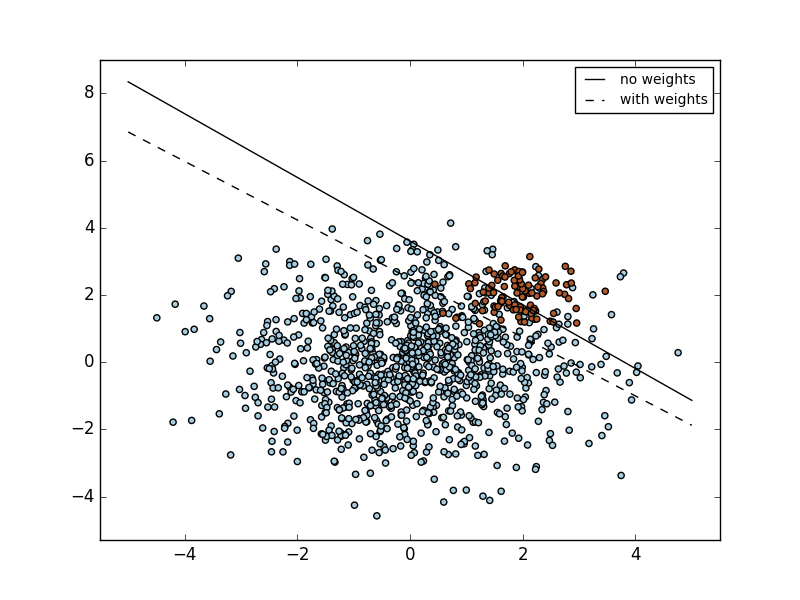
\includegraphics[scale=.5]{SVM1.png}
	\caption{Muestra de desbalance de clases en SVM.}
	\label{SVM1}
\end{figure}

\subsubsection{Formulación matemática}

SVM construye un hiperplano o un conjunto de hiperplanos en un espacio altamente dimensiona, el cual es utilizado tanto para la clasificación de elementos, com para la predicción de valores continuos, a su vez, puede ser implementado para detección de puntos outliers. 

Intuitivamente, se logra una buena separación por el hiper plano que tiene la mayor distancia a los puntos de datos de entrenamiento más cercanos de cualquier clase, ya que en general, cuanto mayor sea la separación, menor será el error de generalización del modelo.

Es posible observar este comportamiento en la Figura \ref{SVM2}

\begin{figure}[!h]
	\centering
	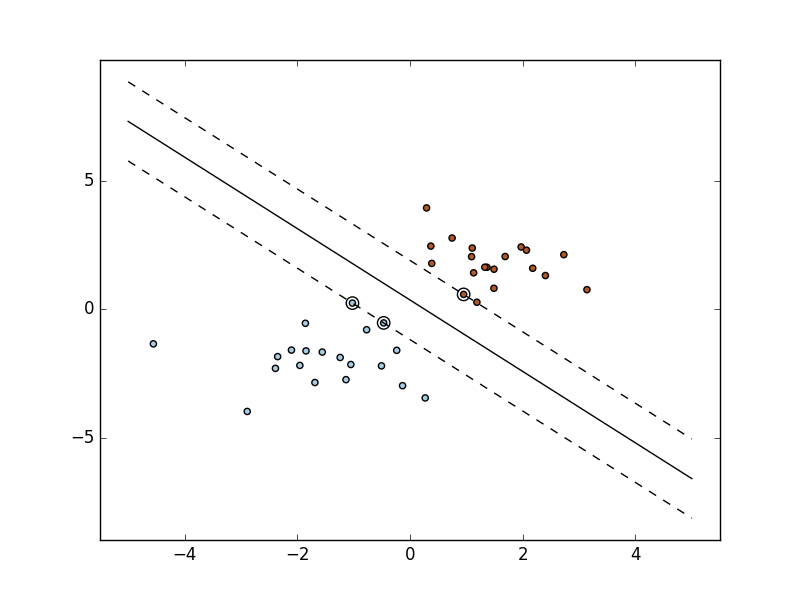
\includegraphics[scale=.5]{SVM2.png}
	\caption{Esquema de hiperplanos en SVM.}
	\label{SVM2}
	
\end{figure}

Es posible entregar una definición matemática para SVM, haciendo una diferenciación asociados a los métodos de clasificación y regresión. De tal manera que, para SVC, se tiene que:

Dado los vectores de entrenamiento $x_{i}\ \in\ R$,
i=1,..., n, en dos clases, y un vector, $y \in \{1, -1\}^n$, SVC resuelve el siguiente problema primario:

\begin{center}
	$\min_ {w, b, \zeta} \frac{1}{2} w^T w + C \sum_{i=1}^{n} \zeta_i$
\end{center}
\begin{center}
	
	$para\ la\ clase\ y_i (w^T \phi (x_i) + b) \geq 1 - \zeta_i,\ \zeta_i \geq 0, i=1, ..., n$	
\end{center}

Su doble es

\begin{center}
	$\min_{\alpha} \frac{1}{2} \alpha^T Q \alpha - e^T \alpha$
\end{center}
\begin{center}
	$para\ la\ clase\ y^T \alpha = 0\ 0 \leq \alpha_i \leq C, i=1, ..., n$
\end{center}

Donde $e$ es el vector de todos los unos, $C > 0$ es el límite superior, $Q$ es una matriz de $n\ x\ n$ definida semipositiva, $Q_{ij} \equiv y_i y_j K(x_i, x_j)$, donde $K(x_i, x_j) = \phi (x_i)^T \phi (x_j)$ es el kernel. Los vectores de entrenamiento son implícitamente mapeados en un espacio dimensional mayor (tal vez infinito) por la función $\phi$.

La función de decisión es:

\begin{center}
	$sgn(\sum_{i=1}^n y_i \alpha_i K(x_i, x) + \rho)$
\end{center}

Por otro lado, $\nu$SVC presenta características similares a SVC. No obstante, el uso del parámetro $\nu$ permite controlar el número de vectores de soporte y errores de entrenamiento. $\nu \in (0, 1]$ y  es un límite superior en la fracción de errores de entrenamiento y un límite inferior de la fracción de vectores de soporte.

A su vez, LinearSVC presenta el mismo comportamiento a SVC. Sin embargo, la gran diferencia es la utilización de un kernel lineal como función de transformación de espacio y evaluación de puntos.

Finalmente, ya que SVM también permite entrenar modelos de regresión particularmente con SVR, una definición matemática de éste se expone como:

Dados los vectores de entrenamiento  $x_{i} \in\ R^n$  
$\varepsilon-SVR$ \cite{smola2004tutorial} resuelve el siguiente problema primario:

\begin{center}
	
	$\min_ {w, b, \zeta, \zeta^*} \frac{1}{2} w^T w + C \sum_{i=1}^{n} (\zeta_i + \zeta_i^*)
	$
\end{center}

\begin{center}
	
	$para\ la\ clase\ y_i - w^T \phi (x_i) - b \leq \varepsilon + \zeta_i,$
\end{center}
\begin{center}
	$w^T \phi (x_i) + b - y_i \leq \varepsilon + \zeta_i^*,\ \zeta_i, \zeta_i^* \geq 0, i=1, ..., n$	
\end{center}

Donde $e$ es el vector para todos, $C >$ 0 es el límite superior, $Q$ es una matriz de $n\ x\ n$ definida semipositiva, $Q_{ij} \equiv K(x_i, x_j) = \phi (x_i)^T \phi (x_j)$ es el kernel. Aquí los vectores de
entrenamiento son implícitamente mapeados en un espacio dimensional mayor (tal vez infinito) por
la función $\phi$.

La función de decisión es:

\begin{center}
	$\sum_{i=1}^n (\alpha_i - \alpha_i^*) K(x_i, x) + \rho$
\end{center}

Como se puede observar, las formulaciones matemáticas, tanto para SVC como SVR son similares. Sin embargo, se diferencian en la función de decisión a utilizar, esto es debido a que SVC es un clasificador, mientras que SVR es un métodos de regresión.

\subsection{Métodos de ensamble}

Los métodos de ensamble, se basan en la combinación de las predicciones obtenidas por varios estimadores, construidos en base a algoritmos de aprendizaje supervisado, con el fin de mejorar la generalización del modelo y aumentar la robustez ante nuevos ejemplos \cite{dietterich2000ensemble}.

Existen dos familias de métodos de ensamble, las cuales se diferencian principalmente en la forma en que combinan los modelos para obtener la medida de desempeño final \cite{kotsiantis2007supervised}:

\begin{enumerate}
	
	\item \textbf{Métodos ponderados}: basados en la construcción de varios estimadores independientes y promediar sus medidas de desempeño, esto mejora el rendimiento debido a que disminuye la variabilidad de las clasificaciones. Ejemplos comunes de esto son Bagging y Random Forest.
	
	\item \textbf{Métodos boosting}: basados en la construcción secuencial de modelos, intentando disminuir el sesgo del modelo combinando diferentes estimadores débiles. Cumple con la filosofía \textit{"la unión de varios modelos débiles, puede construir uno fuerte"}. Ejemplos comunes de esto son AdaBoost y Gradient Tree Boosting.
	
\end{enumerate}

A continuación, se explican brevemente algunos de los algoritmos asociados a la familia de métodos de ensamble.

\subsubsection{Bagging}

Bagging forma parte de los métodos ponderados, en particular, se puede definir como métodos que forman una clase de algoritmos compuestos por varias instancias de un estimador, entrenados en base a subconjuntos aleatorios del set de datos original, ponderando sus predicciones individuales en una respuesta ponderada. El objetivo general de estos métodos es reducir la varianza de un estimador, por medio del proceso de entrenamiento de subconjuntos aleatorios \cite{breiman1996bagging}. 

Existen diferentes formas de generar los subconjuntos aleatorios de entrenamiento, dentro de las cuales se destacan las siguientes.

\begin{itemize}
	
	\item Los subconjuntos aleatorios del conjunto de datos se basan en subconjuntos aleatorios de las muestras, esto se conoce como \textit{"Pasting o Pegado"} \cite{breiman1999pasting}. 
	
	\item Las muestras se extraen con reemplazo, siendo este método conocido como \textit{"Bagging"} \cite{breiman1996bagging}.
	
	\item Los subconjuntos aleatorios del conjunto de datos se basan en subconjuntos aleatorios de las características, esto se conoce como \textit{"subespacios aleatorios"} \cite{barandiaran1998random}.
	
	\item Los subconjuntos aleatorios se crean en base a subconjuntos aleatorios de características y muestras, esto se conoce como \textit{"Random Patches"} \cite{ref10.1007/978-3-642-33460-3_28}.
	
\end{itemize}

\subsubsection{Random Forest \label{rf}}

Random Forest es un método de ensamble ponderado basado en árboles de decisión aleatorios. Conjuntos de diversos clasificadores son creados basados en efectos aleatorios tanto de la extracción de características como de ejemplos, formando subconjuntos de elementos, cada uno de estos aporta con un valor de estimación, el cual es ponderado con los restantes, obteniendo así, la medida general \cite{breiman1998}.

Un esquema representativo del proceso, es como se expone en la Figura \ref{rf1}. En ella, se aprecian que se generan $n$ árboles, los cuales contemplan diferentes cantidades de ejemplos o atributos y la estimación final se basa en una ponderación, ya sea por proceso de votación, en el caso de modelos de clasificación, o simplemente por la media, para modelos de regresión \cite{Breiman2001}.

\begin{figure}[!h]
	\centering
	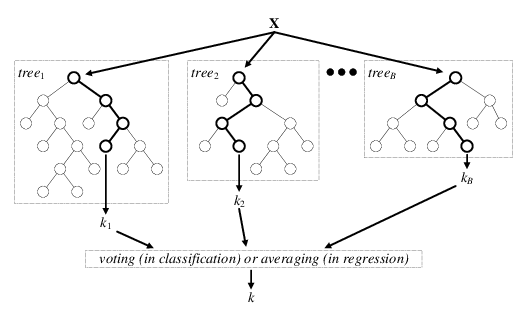
\includegraphics[scale=.5]{rf.png}
	\caption{Esquema representativo de algoritmo Random Forest.}
	\label{rf1}
	
\end{figure}

\subsubsection{AdaBoost}

AdaBoost, es un algoritmo basado en el método boosting, lo que implica que se ajusta a una secuencia de estimadores débiles obtenidos a partir de diferentes subconjuntos de datos generados de manera aleatoria desde el conjunto inicial de datos de entrenamiento \cite{CAO2013745}. 

Cada una de las predicciones obtenidas por los estimadores se combinan de manera ponderada por votación, en el caso de modelos de clasificación, o a través de un promedio en base a las estimaciones resultantes, en el caso de modelos de regresión.

Las modificaciones de los datos en cada iteración de boosting, consisten en aplicar pesos $w_{1},w_{2},..,w_{N}$, a cada una de las muestras de entrenamiento. 

Inicialmente, todos los pesos están configurados en $\Psi_{i}\ =\ 1/N$, de modo que el primer paso simplemente entrena un modelo débil en los datos originales. Para cada iteración sucesiva, las ponderaciones de la muestra se modifican individualmente y el algoritmo de aprendizaje se vuelve a aplicar a los datos ponderados. 

En un paso dado, los ejemplos de entrenamiento que fueron predichos incorrectamente por el modelo mejorado inducido en el paso anterior tienen sus pesos incrementados, mientras que los pesos se disminuyen para aquellos que fueron predichos correctamente \cite{hastie2009multi}. 

A medida que avanzan las iteraciones, los ejemplos que son difíciles de predecir reciben una influencia cada vez mayor. Por lo tanto, cada modelo de aprendizaje débil subsiguiente se ve forzado a concentrarse en los ejemplos que se pierden en los anteriores en la secuencia.

\subsubsection{Gradient Tree Boosting}

Gradient Tree Boosting o Gradient Boosted Regression Trees, es una generalización de métodos de boosting para funciones diferenciables arbitrarias de pérdida \cite{gradient}. Es un método considerado como preciso y efectivo, el cual puede usarse tanto para el desarrollo de modelos de clasificación como de regresión, siendo usado en diferentes áreas de investigación: motores de búsqueda, ecología, minerología, biotecnología, entre otros.

Dentro de las principales ventajas que posee, se encuentran: manejo natural de diferentes tipos de características en un set de datos, alto poder predictivo y robusto frente a la predicción de valores atípicos en una muestra \cite{FRIEDMAN2002367}.

Como formulación matemática, se tiene, la adición de modelos se basa en:

\begin{center}
	$F(x) = \sum_{m=1}^{M} \gamma_m h_m(x)$
\end{center}

Donde $h_{m}(x)$ es una función básica, conocida como \textit{weak learners} en el contexto de boosting. En particular, Gradient Tree Boosting, utiliza árboles de decisión de tamaño fijo como \textit{weak learners}. 


Los modelos aditivos, se construyen de manera incremental, tal que:

\begin{center}
	$F_m(x) = F_{m-1}(x) + \gamma_m h_m(x)$
\end{center}

De tal manera que el nuevo árbol agregado $h_{m}$ trata de minimizar la pérdida $L$ dado el previo ensamble $F_{m-1}$, es decir:

\begin{center}
	$h_m =  \arg\min_{h} \sum_{i=1}^{n} L(y_i, F_{m-1}(x_i) + h(x_i))$
\end{center}

Este algoritmo, resuelve el problema de minimización numéricamente, a través de steepest descent \cite{battiti1992first}. La dirección de steepest descent es el gradiente negativo de la función de pérdida $L$ evaluada en el modelo actual $F_{m-1}$, el cual puede ser calculado para cualquier función de pérdida diferenciable, tal que:

\begin{center}
	$F_m(x) = F_{m-1}(x) - \gamma_m \sum_{i=1}^{n} \nabla_F L(y_i, F_{m-1}(x_i))$
\end{center}

Donde la longitud del paso $\gamma_{m}$ es seleccionada mediante una búsqueda lineal, aplicando:

\begin{center}
	$\gamma_m = \arg\min_{\gamma} \sum_{i=1}^{n} L(y_i, F_{m-1}(x_i) - \gamma \frac{\partial L(y_i, F_{m-1}(x_i))}{\partial F_{m-1}(x_i)})$
\end{center}

A la hora de estimar un valor continuo por medio de algoritmos de regresión o clasificar un nuevo ejemplo a través de un clasificador, existe una única diferencia, la cual radica en la función de pérdida $L$ que es utilizada. En la Tabla \ref{tab:function-loss} se resumen las funciones de pérdida y sus definiciones, normalmente utilizadas en métodos basados en Gradient Tree Boosting.

% Please add the following required packages to your document preamble:
% \usepackage{longtable}
% Note: It may be necessary to compile the document several times to get a multi-page table to line up properly
\begin{longtable}[c]{|l|l|l|}
	\hline
	\multicolumn{3}{|c|}{\textbf{Funciones de pérdida utilizadas en métodos GTB}} \\ \hline
	\endfirsthead
	%
	\endhead
	%
	\multicolumn{1}{|c|}{\textbf{Función}} & \multicolumn{1}{c|}{\textbf{Descripción}} & \multicolumn{1}{c|}{\textbf{Uso}} \\ \hline
	Least squares & \begin{tabular}[c]{@{}l@{}}Valor inicial se obtiene a partir de la\\ media de los vectores respuesta\end{tabular} & Regresión \\ \hline
	Least absolute deviation & \begin{tabular}[c]{@{}l@{}}Valor inicial se obtiene a partir de la\\ mediana de los vectores respuesta\end{tabular} & Regresión \\ \hline
	Huber & \begin{tabular}[c]{@{}l@{}}Combina el uso de mínimos cuadrados\\ y los errores absolutos\end{tabular} & Regresión \\ \hline
	Quantile & \begin{tabular}[c]{@{}l@{}}Se basa en el uso de cuantiles para\\ crear rangos de predicción\end{tabular} & Regresión \\ \hline
	Binomial deviance & \begin{tabular}[c]{@{}l@{}}Se basa en la distribución de probabilidad\\ binomial, para modelos binarios de\\ clasificación\end{tabular} & Clasificación \\ \hline
	Multinomial deviance & \begin{tabular}[c]{@{}l@{}}Se basa en la distribución de probabilidad\\ multinomial y su valor inicial corresponde\\ a las probabilidades a priori de cada\\ categoría\end{tabular} & Clasificación \\ \hline
	Exponential loss & \begin{tabular}[c]{@{}l@{}}Se basa en distribución exponencial y sólo\\ puede ser utilizada en modelos de clasificación\\ binarios\end{tabular} & Clasificación \\ \hline
	\caption{Funciones de pérdida comunes utilizadas en los algoritmos Gradient Tree Boosting, ya sea en forma de clasificador como regresor.}
	\label{tab:function-loss}\\
\end{longtable}

\subsection{Redes Neuronales y Deep Learning}

Redes neuronales es posible definirlas como una serie de modelos de aprendizaje que se basan en la forma de trabajo de las redes neuronales biológicas, es decir, se usa el concepto de \textit{neurona} para estimar una función aproximada, la cual dependerá de un largo número de inputs, generalmente desconocidos.

En la Figura \ref{red} se aprecia un sistema de red neuronal, en la cual se observa un sistema interconectado por neuronas, las cuales intercambian información en forma de mensaje entre ellas, además cada interconexión tiene un peso, el cual es un valor numérico, que puede ser obtenido en base a la experiencia.

En resumen, una red neuronal es un conjunto de entradas y salidas regidas por capas intermedias que permiten evaluar la salida, dichas capas operan entre sí en base a funciones matemáticas y brindan un peso a la conexión, finalmente cada capa es usada para diseñar un modelo de aprendizaje supervisado o no.

\begin{figure}[!h]
	\centering
	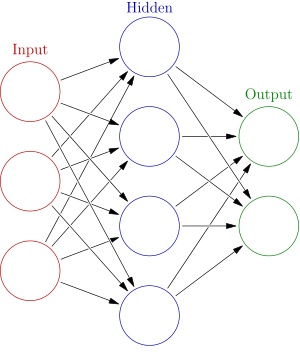
\includegraphics[scale=.5]{red.png}
	\caption{Representación esquemática de una Red Neuronal}
	\label{red}
\end{figure} 

Deep Learning es una herramienta de Machine Learning la cual tiene por objetivo modelar abstracciones de alto nivel en los datos por medio del uso de múltiples capas de procesamiento, ya sea a través del uso de estructuras complejas a través de múltiples transformaciones no lineales \cite{bengio2013representation, MAL-006, SIG-039}. 

La investigación en esta área tiene por objetivo generar mejores representaciones y crear modelos para aprender de éstas a partir de datos no marcados a gran escala. En geneal, las representaciones obtenidas se inspiran en los avances en la neurociencia y se basa libremente en la interpretación de los patrones de procesamiento y comunicación de información en un sistema nervioso, como la codificación neural que intenta definir una relación entre varios estímulos y respuestas neuronales asociadas en el cerebro \cite{MAL-006}.

Deep learning es un método específico de machine learning el cual incorpora redes neuronales organizadas en capas consecutivas para poder aprender iterativamente utilizando un conjunto de datos. Deep learning es especialmente útil cuando se desea aprender patrones provenientes de datos no estructurados \cite{SIG-039}.

Posee diversas arquitecturas, tales como: deep learning network, matrices de convoluciones, redes neuronales recurrentes, etc. las cuales han sido utilizadas en visión artificial para el reconocimiento de patrones, aprendizaje de escritura, etc. Deep Learning es una herramienta de Machine Learning la cual tiene por objetivo modelar abstracciones alto nivel en los datos por medio del uso de múltiples capas de procesamiento, ya sea a través del uso de estructuras complejas a través de múltiples transformaciones no lineales \cite{arel2010deep}.

Dentro de los principales algoritmos que son utilizados en redes neuronales se encuentran Back Propagation \cite{HECHTNIELSEN199265} y Multi Layer Perceptron \cite{80266}.

Si bien en la actualidad, redes neuronales y Deep Learning son metodologías ampliamente utilizadas y han tenido resultados satisfactorios a la hora de trabajar en diferentes áreas de investigación, presentan un problema relevante al momento de aprender de los datos, los atributos y cómo estos facilitan o distribuyen la información.

Este problema es debido a que, los sistemas de redes neuronales trabajan en torno a información oculta, denominados, sistemas de cajas negras, lo cual, no permite comprender cómo se genera una nueva clasificación o predicción de elementos. 

Lo anterior, no ocurre con métodos basados en estimaciones de distancia como KNN, uso de hiperplanos y funciones de kernel para la transformación espacial de los atributos como SVM, reglas de decisión que permiten representar estructuras de árbol que facilitan la comprensión de cómo distribuyen los atributos, rangos preferibles etc., como lo hacen los algoritmos basados en árboles de decisión e inclusive los métodos de ensamble. Es decir, diferentes algoritmos vislumbran cómo manipulan la información para llegar al resultado, no siendo el caso de las redes neuronales. Por lo tanto, dado a que se requiere de algoritmos que permitan la comprensión del problema y que posibiliten generar aprendizaje de los atributos, se descartan a priori el uso de métodos basados en redes neuronales y el uso de Deep Learning.


\subsection{Medidas de desempeño \label{desempeno}}

Medir el desempeño del modelo predictivo es importante a la hora de evaluar qué tan efectivo es el entrenamiento o la clasificación que se genera, existen medidas que sólo se basan en la cantidad de aciertos o errores que comete el clasificador, otras que implican la eficiencia del modelo y otras que se basan en la precisión.

A continuación, se define brevemente algunas de las medidas más utilizadas a la hora de evaluar modelos de aprendizaje supervisados:

\begin{itemize}
	
	\item \textbf{Tasa de Verdaderos Positivos}: corresponde a la medida asociada a las correctas clasificaciones versus el total de clasificaciones realizadas, es decir, cuántas predicciones efectivas se obtuvieron con respecto a una clase.
	
	\item \textbf{Tasa de Falsos Positivos}: corresponde a la medida asociada a las clasificaciones mal efectuadas, es decir, cuántas predicciones erradas existen con respecto a una clase.
	
	
	\item \textbf{Accuracy}: corresponde al total de predicciones correctas con respecto al total de la muestra. Sea $\hat{y}_i$ el valor de predicción del ejemplo $i$ e $y_{i}$ corresponde al verdadero valor, la Accuracy se define como: $\texttt{accuracy}(y, \hat{y}) = \frac{1}{n_\text{samples}} \sum_{i=0}^{n_\text{samples}-1} 1(\hat{y}_i = y_i)$
	
	\item \textbf{Precision}: es la capacidad del clasificador asociada a no etiquetar como positiva una muestra que es negativa, se define como: $\text{precision} = \frac{tp}{tp + fp}$, donde tp corresponde a verdaderos positivos y fp a los falsos positivos.
	
	
	\item \textbf{Recall}: es la capacidad del clasificador asociada encontrar todas las muestras positivas, se define como: $\text{recall} = \frac{tp}{tp + fn}$ , donde tp corresponde a verdaderos positivos y fp a los falsos positivos.
	
	\item \textbf{F-$\beta$}: representa una ponderación armónica entre la Precision y el Recall, se define como: $F_\beta = (1 + \beta^2) \frac{\text{precision} \times \text{recall}}{\beta^2 \text{precision} + \text{recall}}.$ , donde $\beta$ un factor de ponderación.
	
	\item \textbf{Coeficiente de correlación de Matthews}: Se asocia a una medida de la calidad de las clasificaciones, la cual no se ve afectada por el desbalance de clases que pudiese existir, se define como $MCC = \frac{tp \times tn - fp \times fn}{\sqrt{(tp + fp)(tp + fn)(tn + fp)(tn + fn)}}$, donde tp corresponde a verdaderos positivos y fp a los falsos positivos.
	
\end{itemize}
	
Las mediciones expuestas previamente, se utilizan para medir el desempeño de modelos de clasificación, mientras que para evaluar un estimador basado en respuestas continuas, normalmente se utilizan las siguientes:
	
\begin{itemize}
		
	\item \textbf{Coeficiente de Pearson}: Medida lineal entre dos variables cuantitativas aleatorias que permite evaluar el grado de relación entre ellas, se encuentra en rangos entre -1 y 1 donde -1 indica que las variables no presentan relación y 1 que las muestras están estrechamente relacionadas. Se obtiene a partir de $\rho X,Y= \frac{n\sum x_{i}y_{i} - \sum x_{i} \sum y_{i}}{\sqrt{n\sum x^{2}_{i}- (\sum x_{i})^{2}} \sqrt{n\sum y^{2}_{i}- (\sum y_{i})^{2}}}$ donde $x_{i}$ representa los valores de predicción e $y_{i}$ representa los valores reales de la muestra para $n$ ejemplos.
		
	\item \textbf{Coeficiente de Spearman}: Medida de correlación que permite evaluar la asociación o relación entre dos muestras, su interpretación es similar al coeficiente de Pearson y se estima a partir de $\rho = 1- \frac{6\sum D^{2}}{N(N^{2}-1)}$ donde $D$ es la diferencia $x-y$ para el $i-th$ ejemplo y $N$ es el total de ejemplos en la muestra.
		
	\item \textbf{Kendall $\tau$ rank}: Medida que permite evaluar la relación entre dos variables, su interpretación es similar a las basadas en coeficiente de Pearson y Spearman. Se obtiene a partir de $\tau = \frac{\text{(numbers of concordant pairs)} - \text{(number of discordant pairs)}}{n(n-1)/2}$
		
	\item \textbf{Coeficiente de determinación $R^{2}\ score$}: es una medida que cuantifica cómo el predictor se adapta a nuevos ejemplos, posee un rango entre -1 y 1 donde -1 es lo peor y 1 lo mejor, esto es debido a que el estimador puede bajar su rendimiento. Se estima en base a $R^2(y, \hat{y}) = 1 - \frac{\sum_{i=0}^{n_{\text{samples}} - 1} (y_i - \hat{y}_i)^2}{\sum_{i=0}^{n_\text{samples} - 1} (y_i - \bar{y})^2}$ donde $\hat{y}_i$ corresponde al valor predicho para el $i-th$ ejemplo e $y_{i}$ corresponde al valor real en una muestra de $n-samples$.
		
	\item \textbf{Error medio absoluto}: Estima la diferencia positiva entre el valor real y el valor predicho para un conjunto de ejemplos. Se estima a partir de $\text{MAE}(y, \hat{y}) = \frac{1}{n_{\text{samples}}} \sum_{i=0}^{n_{\text{samples}}-1} \left| y_i - \hat{y}_i \right|.$ donde $\hat{y}_i$ corresponde al valor predicho para el $i-th$ ejemplo e $y_{i}$ corresponde al valor real en una muestra de $n-samples$.
		
	\item \textbf{Error cuadrático medio}: Estima la diferencia cuadrática entre el valor real y el valor predicho para un conjunto de ejemplos. Se obtiene a partir de $\text{MSE}(y, \hat{y}) = \frac{1}{n_\text{samples}} \sum_{i=0}^{n_\text{samples} - 1} (y_i - \hat{y}_i)^2$ donde $\hat{y}_i$ corresponde al valor predicho para el $i-th$ ejemplo e $y_{i}$ corresponde al valor real en una muestra de $n-samples$.
		
	\item \textbf{Error logarítmico cuadrático medio}: Es similar al error cuadrático medio, la diferencia principal es que se utiliza el logaritmo natural de las diferencias entre respuesta y valor predicho. Se estima en base a $\text{MSLE}(y, \hat{y}) = \frac{1}{n_\text{samples}} \sum_{i=0}^{n_\text{samples} - 1} (\log_e (1 + y_i) - \log_e (1 + \hat{y}_i) )^2$ donde $\hat{y}_i$ corresponde al valor predicho para el $i-th$ ejemplo e $y_{i}$ corresponde al valor real en una muestra de $n-samples$.
		
	\item \textbf{Error mediano absoluto}: es una medida robusta ante outliers, la pérdida o el error se calcula a partir de las medianas de las diferencias absolutas entre la respuesta y el valor predicho. Se estima en base a $\text{MedAE}(y, \hat{y}) = \text{median}(\mid y_1 - \hat{y}_1 \mid, \ldots, \mid y_n - \hat{y}_n \mid)$ donde $\hat{y}_i$ corresponde al valor predicho para el $i-th$ ejemplo e $y_{i}$ corresponde al valor real en una muestra de $n-samples$.
		
		
\end{itemize}

\subsection{Problemas asociados a los modelos de aprendizaje supervisado \label{problemas}}

Dentro de los principales problemas que pueden presentar los modelos de aprendizaje supervisado, se encuentran las situaciones en las que la cantidad de atributos que puede contener un set de datos es mucho mayor con respecto a la cantidad de ejemplos que se posee, conocido también como \textit{"Maldición de la dimensionalidad"} \cite{indyk1998approximate}.

Es posible definirla como: dado un conjunto de datos $nxm$ con $n$ ejemplos y $m$ descriptores, si $m >> n$, es decir, si $m= n\ x\ n$, es posible que ocurra dicha problemática.

Posibles soluciones a este problema comprenden técnicas asociadas a reducción de dimensionalidad \cite{sarwar2000application, van2009dimensionality}, siendo las más utilizadas \footnote{Estas técnicas, se explican en el capítulo \ref{cap3}}:

\begin{itemize}
	
	\item Métodos lineales de reducción como Análisis de componentes principales (PCA) y derivados.
	\item Análisis de características basados en modelos de clasificación/regresión aplicando Random Forest.
	\item Técnicas probabilísticas asociadas al Mutual Information.
	\item Evaluación de características relacionadas mediante coeficientes de Pearson o matrices de Correlación
\end{itemize}
 
En forma similar, también es posible que un set de datos contemple una gran cantidad de ejemplos y sus descriptores sean escasos. Estos casos se tratan con técnicas de reducción de dimensionalidad y contemplan la eliminación de ejemplos redundantes con el fin de maximizar la variabilidad de los ejemplos, técnicas como Mutual Information, Análisis de Correlaciones son bastante utilizadas en este problema.

Otro posible problema que se puede denotar es el sobreajuste \cite{hawkins2004problem}, esto quiere decir, que el modelo es extremadamente complejo, por lo que éste se ajusta muy bien al set de entrenamiento. No obstante, a la hora de probar con nuevos set de datos no representa la performance obtenida. 

Finalmente, un problema adicional a los modelos de clasificación se basa en el desbalance de clases \cite{japkowicz2002class}. Esto quiere decir, que existe una diferencia significativa entre los contadores de categorías asociadas a las clases, lo cual afecta a los algoritmos a la hora de entrenar, debido a que aumenta el riesgo de cometer errores del tipo I (falsos positivos). Normalmente, esto conlleva a una reducción de ejemplos de la clase mayoritaria en la etapa de entrenamiento o si es posible, la adición de nuevos ejemplos de la clase minoritaria. 

\subsection{Validación de modelos}

La validación de los modelos trata los problemas de sobreajuste y la generalización, es decir, evitar desarrollar modelos que sólo tengan buenas métricas o medidas de desempeño para los datos de entrenamiento y no permitan clasificar nuevos ejemplos. 

Con el fin de poder evitar esta problemática, normalmente los set de datos se dividen en 3 conjuntos: Entrenamiento, validación y testeo. Esto quiere decir, se considera una porción de elementos para entrenar el modelo, una segunda instancia para obtener las medidas de desempeño y una tercera con el fin de determinar si el clasificador entrega resultados acorde a las respuestas conocidas \cite{kohavi1995study}.

Existen técnicas que a partir del set de entrenamiento, generan múltiples divisiones, con el fin de entrenar subconjuntos de elementos del conjunto de entrenamiento y así obtener modelos ponderados.

La subdivisión en $n$ modelos para entrenar y generar modelos ponderados, permite aumentar la generalización del modelo, debido a que las medidas de desempeño varían levemente de aplicación en aplicación y al considerar las divisiones, se tienen distribuciones de las medidas del modelo. Dada las distribuciones, el entrenamiento reporta, la media de dicha distribución \cite{golub1979generalized}. 

Dentro de las principales técnicas de validación se encuentra la Validación cruzada con $k$ divisiones \cite{golub1979generalized} y un caso particular conocido como \textit{Leave one out}, en el cual el valor de $k$ es igual a la cantidad de ejemplos en el entrenamiento \cite{vehtari2017practical}. Éstas se explican a continuación.

\subsubsection{Validación Cruzada}

La validación cruzada, a veces llamada estimación de la rotación, es una técnica de validación del
modelo para evaluar cómo los resultados de un análisis estadístico se generalizarán a un conjunto de datos independiente. 

Se utiliza principalmente en entornos donde la meta es la predicción, y se
quiere estimar la precisión con la que un modelo predictivo se llevará a cabo en la práctica \cite{golub1979generalized}. 

En un problema de predicción, a un modelo se le suele asignar un conjunto de datos, con respuestas conocidas, sobre los que se ejecuta el entrenamiento (conjunto de datos de formación) y un conjunto de datos desconocidos contra los que se prueba el modelo. El objetivo de la validación cruzada es definir un conjunto de datos para \textit{probar} el modelo en la fase de entrenamiento (es decir, el conjunto de datos de validación), con el fin de limitar problemas asociados al sobre ajuste.

La idea es dividir el set de datos en $K$ sub conjuntos, donde por cada subdivisión se entrena con elementos de tamaño $k-1$ y el conjunto restante, es usado para validar el modelo. Una explicación visual del problema, se puede explicar en la Figura  \ref{VC}:

\begin{figure}[!h]
	\centering
	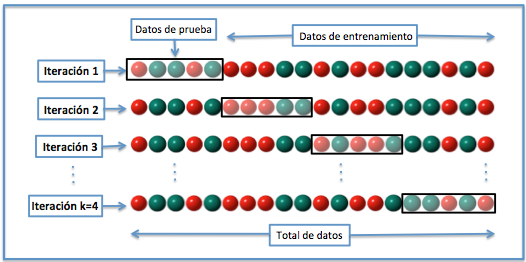
\includegraphics[scale=.5]{validacionCruzada.jpg}
	\caption{Esquema representativo de validación cruzada.}
	\label{VC}
\end{figure}

A modo de ejemplo, sea $K=10$ el número de divisiones a realizar, esto implica, que para un conjunto de datos de tamaño $n$ se forman 10 sub conjuntos de tamaño $n/10$. La validación cruzada implica el entrenamiento y testeo del modelo $K$ veces, en este caso, 10. Por cada iteración, se forma un conjunto de entrenamiento de tamaño $9n/10$ y se testea con un sub conjunto de tamaño $n/10$. 

Por cada iteración, se rota el conjunto de entrenamiento y de testeo, y se obtiene una distribución del desempeño del modelo, reportando el promedio de las métricas asociadas.

\subsubsection{Leave one out}

Es un tipo especial de validación cruzada, en donde se tiene una muestra con $n$ ejemplos en la etapa de entrenamiento se subdivide dicho set de datos considerando $n-1$ elementos, de tal manera que 1 no se considera, la idea en particular radica en entrenar con los $n-1$ ejemplos y validar o testear con el ejemplo restante, esto se itera $n$ veces, tal como se expone en \ref{LOO}, implicando una mayor cantidad de iteraciones que validación cruzada, provocando además un mayor coste computacional \cite{kohavi1995study}.

\begin{figure}[!h]
	\centering
	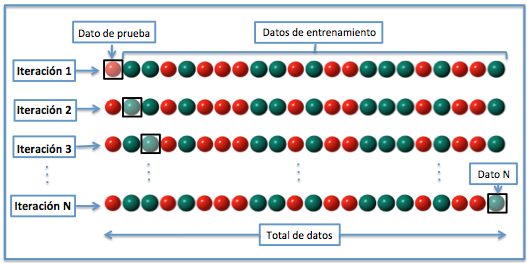
\includegraphics[scale=.5]{Leave-one-out.jpg}
	\caption{Esquema representativo de Leave One.}
	\label{LOO}
\end{figure}

Es decir, es un caso particular de validación cruzada, donde $K=n$ siendo $n$ el número de ejemplos en el conjunto de datos.

Este tipo de validación, provoca disminuciones en las medidas de desempeño, ya que, aumentan la cantidad de puntos en la distribución. Además, en términos computacionales, resulta ser más costosa, por lo que se suele emplear con conjuntos de datos de tamaño bajo, normalmente, menores a 20 ejemplos.

\section{Herramientas computacionales asociadas a evaluación de mutaciones}

Las herramientas computacionales asociadas a la evaluación de mutaciones puntuales se centran principalmente en el análisis de cómo ésta afecta a la estabilidad o la predicción de energía libre asociada a los residuos involucrados en la mutación. Sin embargo, a pesar de que el objetivo es el mismo, se enfocan en diferentes puntos de vista para abordar la problemática, tanto a nivel de entrenamiento de modelos, cómo manipulación de set de datos, así como las técnicas utilizadas para la predicción de los cambios de energía libre.

En la Tabla \ref{tab:tab-summary-tools} se exponen las principales herramientas existentes para la evaluación de la estabilidad de proteínas evaluando mutaciones puntuales, presentando las características, tipos de datos de entrada, resultados, estado de la herramienta y cuáles son las limitantes asociadas

% Please add the following required packages to your document preamble:
% \usepackage{longtable}
% Note: It may be necessary to compile the document several times to get a multi-page table to line up properly
\begin{longtable}[c]{|l|l|l|l|l|}
	\hline
	\multicolumn{1}{|c|}{\textbf{Herr.}}                 & \multicolumn{1}{c|}{\textbf{Características}}                                                                                                                                                                                                                                                                                                                               & \multicolumn{1}{c|}{\textbf{Entradas}}                                                                                                                           & \multicolumn{1}{c|}{\textbf{Salidas}}                                                                                                                                                                                                                         & \multicolumn{1}{c|}{\textbf{Disp.}}                                                  \\ \hline
	\endfirsthead
	%
	\endhead
	%
	Foldx                                                & \begin{tabular}[c]{@{}l@{}}Predice el valor del\\ DDG a través del uso\\ de funciones de energía\\ derivados de términos\\ fisicoquímicos, \\ estadísticos e\\ información estructural\end{tabular}                                                                                                                                                                          & \begin{tabular}[c]{@{}l@{}}Estructura en\\ formato PDB\\ e información\\ sobre la mutación\end{tabular}                                                          & \begin{tabular}[c]{@{}l@{}}Estimación de\\ la diferenciade\\ energía libre\end{tabular}                                                                                                                                                                       & \begin{tabular}[c]{@{}l@{}}Disponible\\ mediante\\ licencia\\ académica\end{tabular} \\ \hline
	I-Mutant                                             & \begin{tabular}[c]{@{}l@{}}Método basado en SVM\\ para la predicción de\\ DDG y la clasificación\\ de la estabilidad de una\\ proteína ante mutaciones\\ puntuales. La mutación es\\ caracterizada a través de\\ propiedades estructurales\\ y la información del\\ ambiente.  Permite la\\ manipulación tanto de\\ secuencias lineales\\ como estructuras PDB\end{tabular} & \begin{tabular}[c]{@{}l@{}}Secuencia lineal\\ proteína, posición\\ y mutación, en\\ caso de existir\\ estructura 3D, se\\ requiere el archivo\\ PDB\end{tabular} & \begin{tabular}[c]{@{}l@{}}Predicción del\\ DDG asociado \\ a la mutación o\\ clasificación\\ de la mutación \\ en estable o\\ desestabilizante\end{tabular}                                                                                                  & \begin{tabular}[c]{@{}l@{}}Disponible\\ para\\ ejecución\\ local\end{tabular}        \\ \hline
	CUPSAT                                               & \begin{tabular}[c]{@{}l@{}}Predice el DDG usando\\ información estructural\\ y del ambiente asociado\\ a la mutación, además\\ utiliza diferentes\\ propiedades estructurales\\ para estimar el valor de\\ energía libre. Este es un\\ método sólo basado en\\ estimaciones utilizando\\ técnicas de\\ bioinformática\\ estructural.\end{tabular}                           & \begin{tabular}[c]{@{}l@{}}Estructura en\\ formato PDB\\ y la posición\\ del residuo a mutar\end{tabular}                                                        & \begin{tabular}[c]{@{}l@{}}Información sobre\\ las 19 posibles\\ sustituciones a\\ realizar, referidas\\ a términos como:\\ ángulos de torsión,\\ accesibilidad\\ al solvente, tipo de\\ estructura\\ secundaria,\\ dentro de las\\ principales.\end{tabular} & No disponible                                                                        \\ \hline
	Dmutant                                              & \begin{tabular}[c]{@{}l@{}}Se basa en el uso de\\ potenciales energéticos\\ para entrenar modelos,\\ utiliza distancias para\\ describir el ambiente y\\ estima el DDG asociado\\ a la mutación\end{tabular}                                                                                                                                                                & \begin{tabular}[c]{@{}l@{}}Estructura en\\ formato PDB\end{tabular}                                                                                              & \begin{tabular}[c]{@{}l@{}}Predicción del\\ DDG asociado\\ a la mutación\end{tabular}                                                                                                                                                                         & No disponible                                                                        \\ \hline
	\begin{tabular}[c]{@{}l@{}}AUTO-\\ MUTE\end{tabular} & \begin{tabular}[c]{@{}l@{}}Manipula las coordenadas\\ de los residuos y aplica\\ triangulación de Delaunay\\ para forma geometrías,\\ así permite describir el\\ ambiente bajo el cual se\\ encuentra el residuo.\\ Los clasificadores se\\ construyen entrenando\\ con Random Forest y\\ los predictores a\\ través de árbolesde\\ decisión.\end{tabular}                  & \begin{tabular}[c]{@{}l@{}}ID-PDB,\\ cadena y\\ mutación\end{tabular}                                                                                            & \begin{tabular}[c]{@{}l@{}}Predicción DDG\\ o clasificación\\ estabilidad,\\ además de\\ información\\ relacionada al\\ sector donde\\ ocurre la\\ mutación\end{tabular}                                                                                      & \begin{tabular}[c]{@{}l@{}}Descargable\\ para\\ ejecución\\ local\end{tabular}       \\ \hline
	\caption{Principales herramientas computacionales enfocadas a la evaluación de la estabilidad o predicción de cambios en la energía libre, asociado a mutaciones puntuales en proteína.
	}
	\label{tab:tab-summary-tools}\\
\end{longtable}

Diferentes son los puntos de vista que pueden ser considerados a la hora de evaluar el efecto que provoca la sustitución de residuos en la estabilidad de una proteína. Ya sea por medio de la estimación utilizando funciones de energía o potenciales energéticos (FoldX \cite{Schymkowitz2005}, Dmutant \cite{Zhou2004}, CUPSAT \cite{Parthiban2006}). Por otro lado, se encuentran métodos basados en algoritmos de apredizaje supervisado. No obstante, estos pueden ser diferenciados con respecto al algoritmo de entrenamiento utilizado o a la forma de describir la mutación. Por ejemplo, I-Mutant \cite{Capriotti2005}, utiliza SVM para predecir o clasificar el efecto de la mutación. Mientras que, AUTO-MUTE \cite{Masso2010} utiliza Random Forest para la clasificación del efecto y Árboles de decisión como algoritmo de regresión.

Cada uno entrega distintas ventajas y desventajas, las cuales se basan principalmente, en la precisión del método y en el tiempo de cómputo relacionado al procedimiento. No obstante, también influye la disponibilidad de estos y si permiten descargas de código fuente para ejecuciones locales o simplemente disponen de versiones web. 


\subsection{Herramientas necesarias para la caracterización de los set de datos}

Adicional a las herramientas expuestas, se hace una descripción breve de SDM \cite{Pandurangan2017} y MOSST \cite{Olivera-Nappa2011}, las cuales serán utilizadas a lo largo de la metodología con el fin de poder caracterizar las mutaciones desde los puntos de vista termodinámico, aplicando SDM y filogenético, por medio de MOSST.

\subsubsection{SDM}

Site Directed Mutator (SDM) \cite{Pandurangan2017}, es una de las herramientas más utilizadas a la hora de evaluar mutaciones puntuales en una proteína de interés y cuyo objetivo principal, es estudiar el efecto sobre la estabiliadd de la proteína que provoca el cambio del residuo.

Se basa en potenciales estadísticos de funciones de energía, para obtener una cuantificación del efecto de una sustitución de un residuo. Este valor se representa por la diferencia de energía libre de Gibbs ($\Delta  \Delta G$). Para estimar el efecto, utiliza ambientes específicos de frecuencias de sustituciones de aminoácidos, sin la utilización de familias de proteínas homólogas. 


Para realizar la estimación, SDM recibe un archivo PDB en el cual se describe la estructura de la proteína inicial, seguido además de la mutación, la cual se describe mediante \textit{"W-Pos-M"}, los cuales corresponden a: Wilde residue, posición en la que se encuentra y mutate residue, respectivamente.

Sus medidas de desempeño en cuanto a la correlación entre los elementos predichos y los reales alcanza un 0.8, calculada a partir del testeo de la herramienta con mutaciones en la proteína Barnasa y staphylococcal nuclease. Este desempeño, lo convierte en una herramienta bastante precisa a la hora de estudiar nuevas predicciones.

Una de las principales razones de utilizar SDM y no otras herramientas computacionales, como las expuestas en la Tabla \ref{tab:tab-summary-tools}, es el hecho de basarse en potenciales estadísticos. Si bien, esta metodología no es tan precisa como el uso de potenciales físicos de funciones de energía, el hecho de utilizar simulaciones basadas en mecanismos de Monte Carlo, conlleva un gran costo computacional en horas de cálculo y recursos. No obstante, es mucho más eficiente que los métodos basados en Machine Learning, dado a que estos, normalmente, tienden a ajustarse y se requiere una gran cantidad de datos para entrenar estos modelos. Además, ya que estos se basan principalmente en métodos asociados a Support Vector Machine (SVM) o Redes Neuronales. Los primeros, no son capaces de adaptarse a espacios altamente no lineales. Mientras que los basados en redes neuronales, no permiten aprender de los atributos empleados, debido a la forma en cómo estos trabajan.

Además, SDM entrega resultados adicionales que permiten comprender el ambiente bajo el cual se produce la mutación y cómo, propiedades termodinámicas se ven afectadas ante la sustitución de residuos.

\subsubsection{MOSST}

Mutagenesis Objetive Search and Selection Tool (MOSST) \cite{Olivera-Nappa2011}, es una herramienta que permite analizar una proteína de interés, con respecto a un conjunto de proteínas con relación filogenética, representadas en un alineamiento múltiple de secuencias. Esto con el fin, de poder detectar posiciones en la proteína de interés o target, que podrían ser mutadas para alterar o no las características de la misma.

Por otro lado , permite estimar mutagénesis relacionadas con la posibilidad de si un cambio de aminoácido dado tendría efectos perjudiciales sobre la proteína. 

Además, como un uso alternativo, es factible la identificación de nsSNPs cuyos fenotipos son relevantes en una familia de genes, permitiendo separar, a aquellas sustituciones que no tienen implicaciones a nivel de funcionalidad.


MOSST aplica técnicas estadísticas para el análisis de las posiciones y se centran en comprender los efectos de las sustituciones desde el punto de vista filogenético. Esto es relevante, ya que como input, sólo necesita secuencias lineales de proteínas, es decir, no es necesario el uso de estructuras en formato PDB, lo cual permite abarcar un mayor número de proteínas de estudio.

Actualmente MOSST se encuentra disponible vía ejecución local, implementado bajo lenguaje de programación Matlab. No obstante, posee una versión online para su uso, facilitando el acceso a la herramienta a diferentes estratos de público.

Utilizar la herramienta MOSST como generación de descriptores basados en propiedades filogenéticas, radica en las ventajas que ésta presenta. Por un lado, permite evaluar la propensión de la mutación y cómo ésta afecta a las características de la proteína en estudio y su familia. Además, permite entender conceptos relacionados a mutaciones, que no son considerados al utilizar propiedades termodinámicas y estructurales. Ya que, estos últimos, sólo evalúan el ambiente bajo el cual ocurre la mutación, mientras que MOSST, evalúa la propensión al cambio. 

El uso de las herramientas MOSST y SDM permitirán describir las mutaciones desde los puntos de vista filogenético y termodinámico-estructural, de tal manera, las falencias de cada método, se complementan, facilitando la generación de descriptores relevantes para las mutaciones.

\section{Hipótesis}

En base a las herramientas existentes y en vista del aumento considerable de datos asociados a mutaciones en proteínas y el conocimiento de las respuestas que éstas generan, se evidencia la necesidad del desarrollo de herramientas computacionales o nuevos modelos de clasificación o regresión que faciliten el entrenamiento de proteínas singulares y la evaluación de sus mutaciones puntuales, con el fin de poder evaluar nuevos ejemplos y cuáles serían los efectos de estos, sin tener que recurrir en grandes costos económicos y tiempos de espera. 

Dado esto se propone la siguiente hipótesis.\\

\textit{El uso de propiedades filogenéticas, termodinámicas y estructurales como descriptores de mutaciones permite el desarrollo de modelos predictivos inspirados en sistemas de meta-learning?}\\

Además de la hipótesis central surgen interrogantes como.

\begin{itemize}
	
	\item Es posible utilizar estos nuevos modelos como herramientas para diagnóstico médico?
	\item Cómo se evalúan la robustez y la generalización de estos modelos, serán capaces de adaptarse a nuevos ejemplos?
	\item Es factible el desarrollo de una herramienta computacional que permita entrenar diferentes set de datos y que facilite la predicción de nuevos ejemplos?
	
\end{itemize}

\section{Objetivos}

En base a la hipótesis planteada y a las preguntas adicionales expuestas, se exponen a continuación el objetivo general y los objetivos específicos.

\subsection{Objetivo general}

Diseñar e implementar estrategias inspiradas en Meta Learning para la implementación de modelos de clasificación y regresión, asociados a mutaciones puntuales en proteínas de interés basados en descriptores termodinámicos, estructurales y filogenéticos.

\subsection{Objetivos específicos}

Dentro de los objetivos específicos se encuentran los siguientes.

\begin{enumerate}
	
	\item Preparar y describir, por medio de propiedades termodinámicas, estructurales y filogenéticas, set de datos de mutaciones puntuales de proteínas con respuesta conocida expuestos en bibliografía o bases de datos públicas.
	
	\item Implementar y evaluar metodología de meta learning para el diseño de meta modelos de clasificación y regresión de mutaciones puntuales aplicados a set de datos de proteínas generadas.
	
	\item Diseñar e implementar herramienta computacional que permita el entrenamiento de set de datos y el uso de meta modelos para la evaluación de nuevos ejemplos.
	
	\item Testear y evaluar comportamiento de la herramienta y los meta modelos en base a sistemas de datos que involucren mutaciones en proteínas con respuesta conocida.
	
	\item Implementar modelos de clasificación para la relevancia clínica de mutaciones puntuales en proteína pVHL, asociada a la enfermedad von Hippel Lindau. 
	
\end{enumerate}

\section{Metodología propuesta}

Con el fin de poder responder a la hipótesis planteada y dar solución a los objetivos impuestos, se propone una metodología general, en la cual, se consideran diferentes estrategias, implementaciones y evaluación de modelos. A continuación se explica la metodología propuesta y los componentes principales de ésta.

\subsection{Preparación de set de datos}

La preparación del set de datos consiste en obtener data para poder entrenar los modelos  predictivos, la data se asocia a información de mutaciones en proteínas y la respuesta que ésta genera. En la Figura \ref{C2:M1} se expone un esquema general con los pasos desarrollados para la preparación del set de datos.

\begin{figure}[!h]
	\centering
	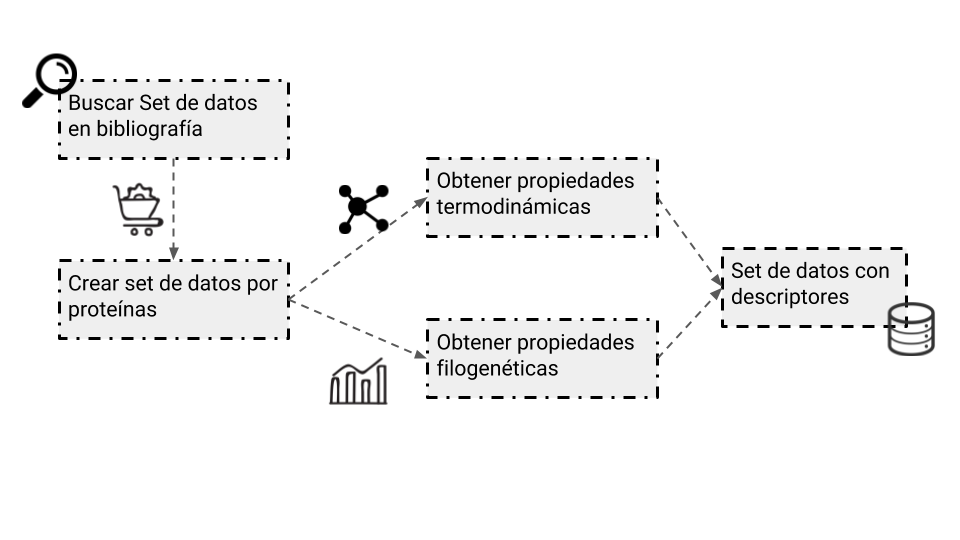
\includegraphics[scale=.4]{m1.png}
	\caption{Esquema representativo asociado al proceso de generación de set de datos de mutaciones puntuales en proteínas.}
	\label{C2:M1}
\end{figure}

Tal como se expone en la Figura \ref{C2:M1}, los set de datos se buscan en la bibliografía, a partir de modelos desarrollados previamente, bases de datos, en la literatura, etc. El objetivo fundamental, es encontrar proteínas con mutaciones puntuales cuyo efecto sea conocido, dicha respuesta puede ser categórica, es decir, asociada al diseño e implementación de modelos de clasificación o continua y se aplica para modelos de regresión. 

En una segunda instancia, a partir de la data recolectada, ésta se procesa con el fin de poder obtener set de datos de proteínas individuales con una cantidad de ejemplos considerables que permitan el diseño de modelos válidos, para ello, fueron implementados scripts bajo el lenguaje de programación Python con el fin de recuperar las proteínas, obtener la información y generar la data de manera individual, además, eliminar ejemplos ambiguos. Es decir, filas con los mismos valores pero cuya columna de respuesta fuese diferente. 

A partir de esto, se forman $n$ set de datos asociados a $n$ proteínas, cada uno con $m$ ejemplos y cuyos descriptores consisten en el residuo original, posición en proteína, residuo mutado y la respuesta asociada. El desbalance de clases se analiza con respecto a las posibles categorías existentes en la respuesta y el porcentaje de representatividad que éstas poseen en la muestra. Se considera que el set de datos exhibe este comportamiento cuando presentan las características expuestas en la sección \ref{problemas}. En el caso de detectar esta problemática, el conjunto de datos será tratado empleando el método SMOTE (Synthetic Minority Oversampling Technique) \cite{chawla2002smote}.

Posteriormente, se aplican las herramientas SDM \cite{Pandurangan2017} y MOSST \cite{Olivera-Nappa2011} con el fin de obtener los descriptores asociados a las propiedades termodinámicas y filogenéticas, respectivamente. Para ello, scripts implementados en lenguaje de programación Python, son desarrollados para consumir los servicios de dichas herramientas y registrar los resultados obtenidos, formando así, set de datos con los descriptores planteados en los objetivos iniciales. Un punto importante a destacar, es que el uso de SDM implica que las proteínas a trabajar, deben presentar una estructura 3D reportada en el Protein Data Bank \cite{berman2000protein} o al menos poseer un modelo representativo y validado. Esto es debido a que se utilizan informaciones de coordenadas para la estimación del efecto de la mutación, minimizaciones energéticas y estabilización de la mutante.

Ya con los descriptores formados, las características asociadas a variables categóricas son codificadas. Si la totalidad de posibles categorías supera el 20\% del total de características en el set de datos, se aplica Ordinal Encoder, en caso contrario, One Hot Encoder \cite{pedregosa2011scikit}. Ordinal Encoder consiste en la transformación de variables categóricas en arreglos de números enteros con valores desde $0,...,n-1$ para $n$ posibles categorías. Por otro lado, One Hot Encoder, consiste en agregar tantas columnas como posibles categorías existan en el set de datos completadas mediante binarización de elementos (0 si la característica no se presencia, 1 en caso contrario)\footnote{Más detalles sobre la codificación de variables categóricas y secuencias lineales de proteínas serán tratadas en el capítulo \ref{cap3}.}.

Es importante mencionar, que las respuestas asociadas a las mutaciones pueden ser del tipo continuo o categórico, lo cual implica que tanto los modelos como las métricas varían. No obstante, se aplica la metodología indistintamente, con el fin de demostrar la robustez del método y la eficacia de éste sin importar el tipo de modelo que se éste entrenando.

\subsection{Implementación de meta modelos de clasificación/regresión}

La implementación de meta modelos consiste en la obtención de un grupo de estimadores que en conjunto, permiten clasificar o predecir nuevos ejemplos. Para ello, se diseña e implementa una metodología inspirada en Sistemas de Meta Learning y aplicando técnicas estadísticas para la evaluación del desempeño y el uso del meta modelo con nuevos ejemplos.

En la Figura \ref{C2:M2}, se exponen las etapas asociadas a la implementación de meta modelos, contemplando desde la fase de entrenamiento de los modelos hasta la unión en meta clasificadores, lo cual se reporta en la herramienta MLSTools (Paper en redacción). 

Cada una de las etapas, contempla un conjunto de scripts implementados en lenguaje de programación Python y empleando la librería Scikit-Learn para el entrenamiento y evaluación de los clasificadores o predictores \cite{pedregosa2011scikit}, así como Numpy para el uso de módulos estadísticos \cite{doi:10.1109/MCSE.2011.37}.


\begin{figure}[!h]
	\centering
	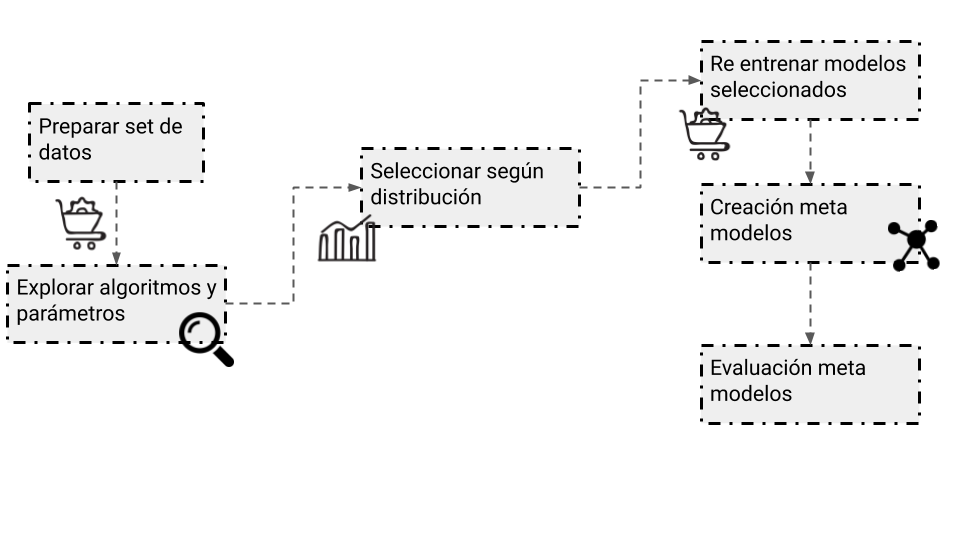
\includegraphics[scale=.4]{m2.png}
	\caption{Esquema representativo asociado al proceso de creación de meta modelos utilizando la metodología reportada para la herramienta MLSTools (Paper en redacción).}
	\label{C2:M2}
\end{figure}

Tal como se observa en la Figura \ref{C2:M2}, es posible identificar etapas claves en el proceso: Exploración de modelos, Selección y Generación de los meta clasificadores/predictores, junto con su evaluación. Cada una de estas etapas se exponen a continuación.

\subsubsection{Exploración de modelos}

La exploración de modelos o estimadores, se basa en la aplicación de diferentes algoritmos de aprendizaje supervisado con variaciones en sus parámetros de configuración inicial. La utilización de los algoritmos, depende principalmente del tipo de respuesta que presente el set de datos, es decir, si es continua o categórica. No obstante, a modo resumen, en la Tabla \ref{cap2:tab1} se exponen los algoritmos utilizados, el caso en el que se usan y los parámetros que se varían junto con el total de iteraciones posibles para cada elemento:

\begin{longtable}[c]{llll|l|l|}
	\hline
	\multicolumn{6}{|c|}{\textbf{Algoritmos y parámetros empleados en la etapa de Exploración en MLSTools}}                                                                                                                                                                                                                                                                                               \\ \hline
	\endfirsthead
	%
	\endhead
	%
	\multicolumn{1}{|l|}{\textbf{\#}} & \multicolumn{1}{l|}{\textbf{Algoritmo}}                                                  & \multicolumn{1}{l|}{\textbf{Tipo}}    & \textbf{Parámetros}                                                                                                                 & \textbf{Uso}                                                         & \textbf{Iteraciones} \\ \hline
	\multicolumn{1}{|l|}{1.}          & \multicolumn{1}{l|}{Adaboost}                                                            & \multicolumn{1}{l|}{Ensamble}         & \begin{tabular}[c]{@{}l@{}}Algoritmo\\ Número estimadores\end{tabular}                                                              & \begin{tabular}[c]{@{}l@{}}Clasificación \\ y Regresión\end{tabular} & 16                   \\ \hline
	\multicolumn{1}{|l|}{2.}          & \multicolumn{1}{l|}{Bagging}                                                             & \multicolumn{1}{l|}{Ensamble}         & \begin{tabular}[c]{@{}l@{}}Bootstrap\\ Número estimadores\end{tabular}                                                              & \begin{tabular}[c]{@{}l@{}}Clasificación y\\ Regresión\end{tabular}  & 16                   \\ \hline
	\multicolumn{1}{|l|}{3.}          & \multicolumn{1}{l|}{\begin{tabular}[c]{@{}l@{}}Bernoulli\\ Naive Bayes\end{tabular}}     & \multicolumn{1}{l|}{Probabilístico}   & Default                                                                                                                             & Clasificación                                                        & 1                    \\ \hline
	\multicolumn{1}{|l|}{4.}          & \multicolumn{1}{l|}{Decision Tree}                                                       & \multicolumn{1}{l|}{Características}  & \begin{tabular}[c]{@{}l@{}}Criterio división\\ Función de impureza\end{tabular}                                                     & \begin{tabular}[c]{@{}l@{}}Clasificación y\\ Regresión\end{tabular}  & 4                    \\ \hline
	\multicolumn{1}{|l|}{5.}          & \multicolumn{1}{l|}{\begin{tabular}[c]{@{}l@{}}Gaussian\\ Naive Bayes\end{tabular}}      & \multicolumn{1}{l|}{Ensamble}         & Default                                                                                                                             & \begin{tabular}[c]{@{}l@{}}Clasificación y\\ Regresión\end{tabular}  & 1                    \\ \hline
	\multicolumn{1}{|l|}{6.}          & \multicolumn{1}{l|}{\begin{tabular}[c]{@{}l@{}}Gradient\\ Tree Boosting\end{tabular}}    & \multicolumn{1}{l|}{Ensamble}         & \begin{tabular}[c]{@{}l@{}}Función de pérdida\\ Número estimadores\end{tabular}                                                     & \begin{tabular}[c]{@{}l@{}}Clasificación y\\ Regresión\end{tabular}  & 16                   \\ \hline
	\multicolumn{1}{|l|}{7.}          & \multicolumn{1}{l|}{\begin{tabular}[c]{@{}l@{}}k-Nearest\\ Neighbors\end{tabular}}       & \multicolumn{1}{l|}{Distancias}       & \begin{tabular}[c]{@{}l@{}}Número Vecinos\\ Algoritmo\\ Métrica distanciaPesos\end{tabular}                                         & \begin{tabular}[c]{@{}l@{}}Clasificación y\\ Regresión\end{tabular}  & 160                  \\ \hline
	\multicolumn{1}{|l|}{9.}          & \multicolumn{1}{l|}{\begin{tabular}[c]{@{}l@{}}Nu Support\\ Vector Machine\end{tabular}} & \multicolumn{1}{l|}{Kernel}           & \begin{tabular}[c]{@{}l@{}}Kernel\\ Nu\\ Grado polinomio\end{tabular}                                                               & \begin{tabular}[c]{@{}l@{}}Clasificación y\\ Regresión\end{tabular}  & 240                  \\ \hline
	\multicolumn{1}{|l|}{10.}         & \multicolumn{1}{l|}{Random Forest}                                                       & \multicolumn{1}{l|}{Ensamble}         & \begin{tabular}[c]{@{}l@{}}Número estimadores\\ Función de impureza\\ Bootstrap\end{tabular}                                        & \begin{tabular}[c]{@{}l@{}}Clasificación y\\ Regresión\end{tabular}  & 32                   \\ \hline
	\multicolumn{1}{|l|}{11.}         & \multicolumn{1}{l|}{\begin{tabular}[c]{@{}l@{}}Support\\ Vector Machine\end{tabular}}    & \multicolumn{1}{l|}{Kernel}           & \begin{tabular}[c]{@{}l@{}}Kernel\\ C\\ Grado polinómio\end{tabular}                                                                & \begin{tabular}[c]{@{}l@{}}Clasificación y\\ Regresión\end{tabular}  & 240                  \\ \hline
	&                                                                                          &                                       &                                                                                                                                     & \textbf{Total Iteraciones}                                           & \textbf{726}        \\ \cline{5-6} 
	\caption{Tabla resumen, algoritmos implementados, parámetros utilizados e iteraciones involucradas por cada algoritmo.}
	\label{cap2:tab1}\\
\end{longtable}

Como se observa en la Tabla \ref{cap2:tab1}, son sobre 720 modelos los que se generan y a partir de ellos se obtiene distribuciones de medidas de desempeño que permiten evaluarlos. En el caso de modelos de regresión se utilizan los coeficientes de Pearson, Spearman, Kendall $\tau$ y $R^{2}$, mientras que para modelos de clasificación, se consideran la Precisión, Exactitud, Recall y F1.

Finalmente, esta etapa, entrega set de modelos entrenados y evaluados según las métricas de interés. Se destaca que cada modelo es validado a través del proceso de validación cruzada, con el fin de poder disminuir posibles sobreajustes. El valor de $k$ asociado a las subdivisiones a realizar varía con respecto a la cantidad de ejemplos que presente el set de datos, es decir, sea $n$ la cantidad de ejemplos en la muestra, si $n<=20$ se tiene que $k=n$ implicando el uso de Leave one out, si $n>20$ y $n<=50$ se considera un valor de $k=3$, si $n>50$ y $n<=100$ $k=5$, por último, si $n>100$ se tiene un valor de $k=10$.

\subsubsection{Selección de modelos}

Cada distribución de medida de desempeño perteneciente a los modelos entrenados en la fase de Exploración, se somete a test estadísticos basados en Z-score \cite{pedregosa2011scikit} que permite seleccionar los modelos cuyas métricas representen outliers positivos dentro de la distribución.

El algoritmo general, utilizado para el desarrollo de esta selección es como se expone en el algoritmo \ref{alg:select}, para el cual se detallan los pasos simplificados que permiten obtener un conjunto de modelos entrenados y que representan los valores más altos dentro de su distribución. Es importante mencionar, que se obtiene un conjunto $M'$ con los modelos, considerando como punto de selecciones los valores evaluados con respecto a la desviación estándar, considerando los umbrales 3 $\sigma$, 2 $\sigma$ y 1.5 $\sigma$ por sobre la media, si ningún factor se cumple, sólo se considera el valor máximo en la distribución.

Es importante mencionar, que cada distribución puede permitir la selección de distintos modelos, lo cual implica que un mismo modelo pueda ser seleccionado en diferentes medidas, razón por la cual, a la hora de obtener el conjunto de modelos $M'$ se remueven aquellos elementos que se encuentran repetidos. Siendo estos, sólo los modelos que presenten igualdad tanto en el algoritmo como en sus parámetros de configuración inicial.

\begin{algorithm}[H]
	\begin{algorithmic}[1]
		\REQUIRE Conjunto $M$ con modelos entrenados y sus medidas de desempeño, Lista $L$ con medidas de desempeño. \label{lin:lineaRara}
		\ENSURE Conjunto $M'$ con modelos seleccionados.
		
		
		\FOR{$i$ en $L$} 
		\STATE Calcular  media $\mu$, desviación estándar $\sigma$ en distribución $M_{i}$
		\FOR{$ x \in M_{i}$}
		\IF {$x \ge \mu + 3*\sigma$}
		\STATE Agregar $x$ a $M'$
		\ENDIF
		\ENDFOR
		\IF {largo $M'$ = 0}
		\FOR{$ x \in M_{i}$}
		\IF {$x \ge \mu + 2*\sigma$}
		\STATE Agregar $x$ a $M'$
		\ENDIF
		\ENDFOR
		
		\IF {largo $M'$ = 0}
		\FOR{$ x \in M_{i}$}
		\IF {$x \ge \mu + 1.5*\sigma$}
		\STATE Agregar $x$ a $M'$
		\ENDIF
		\ENDFOR
		
		\IF {largo $M'$ = 0}
		\FOR{$ x \in M_{i}$}
		\IF {$x = MAX{M_{i}}$}
		\STATE Agregar $x$ a $M'$
		\ENDIF
		\ENDFOR
		\ENDIF
		\ENDIF
		\ENDIF
		\ENDFOR
		
		\RETURN $D$ sin valores extremos
	\end{algorithmic}
	\caption{Algoritmo de selección de modelos}\label{alg:select}
\end{algorithm}

\subsubsection{Generación y evaluación de meta modelos}

A partir del conjunto de modelos $M'$, el cual representa los estimadores seleccionados, cuyas medidas de desempeño son las más altas en sus distribuciones correspondientes, se generan meta modelos, es decir, estimadores compuestos de diversas unidades, los cuales en conjunto entregan una respuesta, ya sea por ponderación o votación. El proceso general para la generación de los meta modelos, es descrito a continuación.

En una primera instancia, los modelos son nuevamente entrenados y se comparan las nuevas medidas de desempeño con las obtenidas previamente. En caso de que exista una diferencia mayor al 20\%, en cualquiera de sus métricas, el modelo se remueve del conjunto $M'$. La razón fundamental de esto, es debido a que se espera desarrollar modelos robustos cuyas evaluaciones no presenten variaciones significativas y que realmente no alteren sus predicciones ante nuevos ejemplos, razón por la cual, se aplica nuevamente validación cruzada para validar los modelos.

Con el fin de evaluar el desempeño de los meta modelos, nuevas medidas se generan a partir de la información resultante de los modelos individuales. No obstante, la forma en la que se obtienen varían dependiendo del tipo de respuesta que se debe entregar.

Si la respuesta es continua, se obtiene los valores de predicción de cada modelo y se promedian, para luego aplicar las métricas estándar (Coeficiente de Pearson, Kendall $\tau$, Spearman y $R^{2}$) sobre estos valores promediados y los reales. Expresado matemáticamente:

Sea $M'$ la cantidad de elementos en el meta modelo, $n$ la cantidad de ejemplos en el set de datos y sea $Y$ el vector de respuestas reales de tamaño $n$. Para cada $M'_{i}\ \in\ M'$ se obtiene un vector $Y_{i}$ que representa los valores de predicción entregados por el modelo $M'_{i}$. A partir de cada $Y_{i}$ se genera una matriz de predicciones $P(mxn)$ donde $m$ representa la cantidad de modelos en $M'$. Finalmente, se obtiene un vector $Y'$ de tamaño $n$, el cual se compone de la media de cada columna en la matriz $P$, es decir, para el ejemplo $i$ se obtienen $m$ predicciones, las cuales son promediadas, formando el valor $Y'_{i}\ \in\  Y'$. Vector el cual, se utiliza para obtener las métricas de desempeño.

Para el caso en que la respuesta sea categórica, es decir, los modelos son del tipo clasificación, se obtiene la respuesta de cada modelo individual y se selecciona una única categoría, correspondiente a aquella que presente una mayor probabilidad de ocurrencia dada la distribución de elementos y considerando para ello las probabilidades iniciales de cada categoría en el set de datos de estudio. De esta forma, se obtiene un vector respuesta con la clasificación de cada ejemplo cuyo valor corresponde al evento más probable a ocurrir, este vector se compara con el set de respuestas reales y se aplican las métricas de interés para clasificadores.

\subsection{Cómo usar los meta modelos para la clasificación de nuevos ejemplos?}

Nuevos ejemplos pueden ser clasificados o predecir su respuesta, dependiendo sea el caso, a partir de los meta modelos desarrollados. En el caso de estimadores basados en variables continuas, los nuevos ejemplos se someten a cada uno de los modelos individuales pertenecientes al sistema, los cuales generan una respuesta individual, a partir de dichas respuestas, se genera un intervalo de confianza con un nivel de significancia $\alpha=0.01$ donde existe una mayor probabilidad de que se encuentre el valor real de la predicción dado los valores del entrenamiento. Para ejemplos que impliquen clasificación, se obtiene la respuesta de cada modelo individual y se evalúa la probabilidad de ocurrencia de cada categoría, entregando así, la respuesta condicionada por una probabilidad de ocurrencia del evento.

\subsection{Uso de meta modelos en sistemas de proteínas}

El objetivo principal de esta metodología, radica en el hecho de crear una herramienta que permita implementar modelos basados en algoritmos de aprendizaje supervisado para set de datos de mutaciones puntuales o variantes para una misma proteína. 

Un flujo general del uso de la herramienta, se expone en la Figura \ref{C2:M3}.

\begin{figure}[!h]
	\centering
	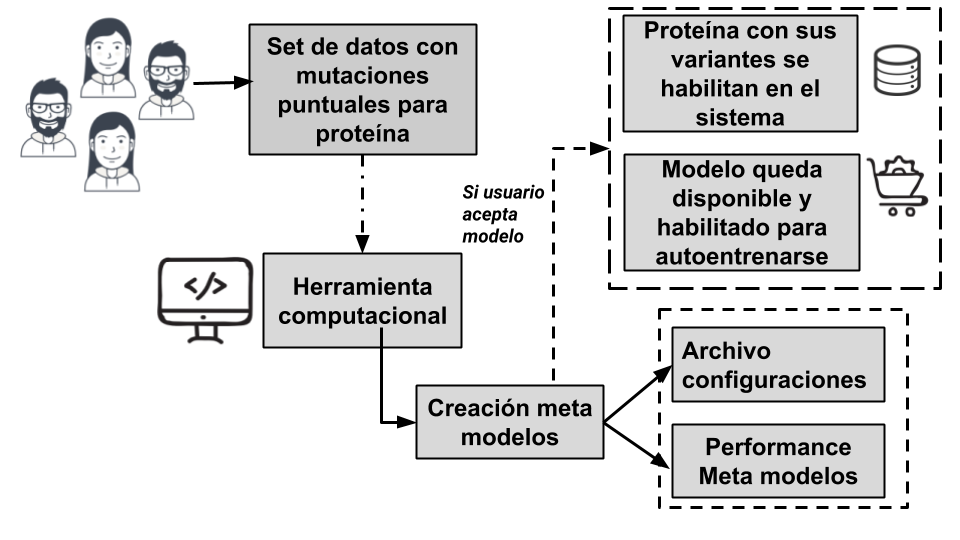
\includegraphics[scale=.4]{m3.png}
	\caption{Esquema representativo de flujo asociado a la herramienta de generación de meta modelos para mutaciones puntuales en proteínas de interés.}
	\label{C2:M3}
\end{figure}

La idea general, consiste en que usuarios de la herramienta, puedan entrenar sus propios modelos de clasificación o regresión, basados en la metodología expuesta en los pasos anteriores mediante el uso de Meta Learning Sytem Tools (Paper en Redacción). Para ello, los usuarios deben entregar sus set de datos con la información necesaria para ser procesada: cadena, residuo original, posición, residuo mutado y respuesta o efecto de la mutación, además del archivo PDB a ser procesado. 

La herramienta, aplica los pasos expuestos en la metodología de este capítulo generando un meta modelo basado en algoritmos de aprendizaje supervisado y las medidas de desempeño que permiten evaluar el modelo obtenido. 

Si el usuario acepta la metodología y permite la publicación de los datos, el sistema habilita el acceso tanto a los meta modelos como a los set de datos y los agrega a la lista de procesos de modelos auto entrenables.

Esto último, implica que ante la adición de nuevos ejemplos al set de datos, el sistema actualiza los modelos y las medidas de desempeño, aplicando la metodología expuesta, así, constantemente mantiene la actualización de la información y permite mantener en constante crecimiento los datos que contemplan el desarrollo de los modelos.

\section{Análisis y evaluación de los set de datos a utilizar}

A continuación, se exponen los resultados obtenidos hasta el momento, presentando principalmente, los set de datos a utilizar, las características que estos poseen y qué representan, con el fin de contextualizar la data a manipular y los modelos a generar.

\subsection{Set de datos utilizados}

En el presente apartado se describen las características básicas de los set de datos trabajados, así como también, qué representan las proteínas bajo las cuales se están desarrollando los modelos de estimadores.

\subsubsection{Descripción general}

Los set de datos utilizados, tanto para la formación de los inputs asociados al sistema, así como también la validación de respuesta correspondiente a la mutación que estos tienen, fueron extraídos desde distintas bases de datos de mutaciones en proteínas de estudios relacionados a los cambios que provoca la sustitución del residuo inicial, ya sea a nivel de cambios energéticos o estabilidad de la proteína.

11 set de datos con respuesta continua fueron obtenidos. Cada set de datos contemplaba como elemento a predecir, las diferencias de energía libre de Gibbs, entre los residuos originales y mutados. Las mutaciones fueron seleccionadas desdes diversos estudios en los cuales se reportaron, centrándose en \cite{Wainreb2011, Sun2017, petukh2016saambe, Alexov2012,prot20185}.

Adicional a los set de datos con respuesta continua, 8 conjuntos de elementos asociados a tareas de clasificación fueron obtenidos desde diversos estudios reportados a la actualidad \cite{ancien2018prediction, broom2017computational, capriotti2008three, quan2016strum, Capriotti2005, 1gzp030, Khan2010, masso2008accurate, getov2016saafec}. 

De tal manera, se generó un total de 19 conjuntos de set de datos, con respuesta categórica y continua, los cuales se asocian a proteínas independientes, usadas para la evaluación de las metodologías planteadas. Estas 19 proteínas junto con su descripción, se exponen en la Tabla \ref{cap2:tab2}.


\begin{longtable}[c]{|l|l|l|l|l|}
	\hline
	\multicolumn{5}{|c|}{\textbf{Resumen set de datos de proteínas y sus características}}                                                                                                                                                                                             \\ \hline
	\endfirsthead
	%
	\endhead
	%
	\textbf{\#} & \textbf{Código PDB} & \textbf{Tipo} & \textbf{Ejemplos} & \textbf{Descripción}                                                                                                                                                                                       \\ \hline
	1.          & 1A22                & Regresión     & 132               & \begin{tabular}[c]{@{}l@{}}Human growth hormone bound to single\\ receptor\end{tabular}                                                                                                                    \\ \hline
	2.          & 1CH0                & Regresión     & 191               & \begin{tabular}[c]{@{}l@{}}Crystal and molecular structures of the complex\\ of alpha-*Chymotrypsin with its inhibitor Turkey\\ Ovomucoid third domain\end{tabular}                                        \\ \hline
	3.          & 1DKT                & Regresión     & 119               & \begin{tabular}[c]{@{}l@{}}CKSHS1: Human cyclin dependent\\ kinase subunit, type 1 complex with\\ metavanadate\end{tabular}                                                                                \\ \hline
	4.          & 1FKJ                & Regresión     & 219               & \begin{tabular}[c]{@{}l@{}}Atomic structure of FKBP12-FK506, \\ an immunophilin  immunosupressant\\ complex\end{tabular}                                                                                   \\ \hline
	5.          & 1FTG                & Regresión     & 203               & \begin{tabular}[c]{@{}l@{}}Structure of apoflavodoxin: closure of\\ a Tyr/Trp aromatic gate leads to a\\ compact fold\end{tabular}                                                                         \\ \hline
	6.          & 1PPF                & Regresión     & 190               & \begin{tabular}[c]{@{}l@{}}X-Ray crystal structure of the complex\\ of human leukocyte elastase and the\\ third domain of the Turkey ovomucoid\\ inhibitor\end{tabular}                                    \\ \hline
	7.          & 1RX4                & Regresión     & 556               & \begin{tabular}[c]{@{}l@{}}Dihydrofolate reductase (E.C.1.5.1.3) complexed\\ with 5,10-Dideazatetrahydrofolate and\\ 2'-Monophosphadenosine 5'-Diphosphoribose\end{tabular}                                \\ \hline
	8.          & 1WQ5                & Regresión     & 239               & \begin{tabular}[c]{@{}l@{}}Crystal structure of tryptophan synthase\\ alpha-subunit from Escherichia coli\end{tabular}                                                                                     \\ \hline
	9.          & 2AFG                & Regresión     & 134               & Human acidic fibroblast growth factor                                                                                                                                                                      \\ \hline
	10.         & 3SGB                & Regresión     & 191               & \begin{tabular}[c]{@{}l@{}}Structure of the complex of Streptomyces\\ Griseus protease B and the Third domain\\ of the Turkey ovomucoid inhibitor\end{tabular}                                             \\ \hline
	11.         & 5AZU                & Regresión     & 203               & \begin{tabular}[c]{@{}l@{}}Crystal structure analysis of oxidize\\ Pseudomonas Aeruginoa Azurin at PH 5.5\\ and PH 9.0. A PH-induced conformational\\ Transition involves a peptide bond flip\end{tabular} \\ \hline
	12.         & 1BN1                & Clasificación & 1802              & Carbonic anhydrase II inhibitor                                                                                                                                                                            \\ \hline
	13.         & 1BVC                & Clasificación & 561               & \begin{tabular}[c]{@{}l@{}}Structure of a Biliverdin Apomyoglobin\\ complex\end{tabular}                                                                                                                   \\ \hline
	14.         & 1LZ1                & Clasificación & 848               & \begin{tabular}[c]{@{}l@{}}Human Lysozyme. Analysis of Non-Bonded\\ and Hydrogen-Bond interactions\end{tabular}                                                                                            \\ \hline
	15.         & 1STN                & Clasificación & 2193              & \begin{tabular}[c]{@{}l@{}}The crystal structure of Staphylococcal\\ Nuclease\end{tabular}                                                                                                                 \\ \hline
	16.         & 1VQB                & Clasificación & 820              & \begin{tabular}[c]{@{}l@{}}Gene V Protein (Single-Stranded DNA\\ Binding Protein)\end{tabular}                                                                                                             \\ \hline
	17.         & 2CI2                & Clasificación & 741               & \begin{tabular}[c]{@{}l@{}}Crystal and molecular structure of the\\ Serine proteinase inhibitor CI-2 from\\ Barley seeds\end{tabular}                                                                      \\ \hline
	18.         & 2LZM                & Clasificación & 2336              & Structure of Baceriophage T4 Lysosyme                                                                                                                                                                      \\ \hline
	19.         & 2RN2                & Clasificación & 712               & \begin{tabular}[c]{@{}l@{}}Structural details of ribonuclease H from\\ Escherichia Coli\end{tabular}                                                                                                       \\ \hline
	\caption{Resumen de proteínas utilizadas para el desarrollo de meta modelos basados en metodología Meta Learning System propuesta durante este capítulo.}
	\label{cap2:tab2}\\
\end{longtable}

Cada una de las proteínas presentan diferentes características y funcionalidades, algunas facilitan la unión a DNA, mientras que otras presentan propiedades enzimáticas, por otro lado, existen enzimas que representan inhibidores, entre las principales. Esto es interesante a la hora de evaluar el poder que presenta la metodología con respecto al análisis de diferentes proteínas, estructuras y complejos, ya que se presenta una gran variedad en cuanto a forma y funcionalidad de éstas, lo que implica que el sistema no se limita por cierto tipo de estructuras o complejos.

A modo de ilustrar las diferencias estructurales de las proteínas en estudio, en la Figura \ref{fig:proteins} se exponen algunas de las estructuras asociadas a las proteínas utilizadas para desarrollar modelos de clasificación o regresión.

\begin{figure}
	\centering
	\begin{subfigure}{0.4\textwidth}
		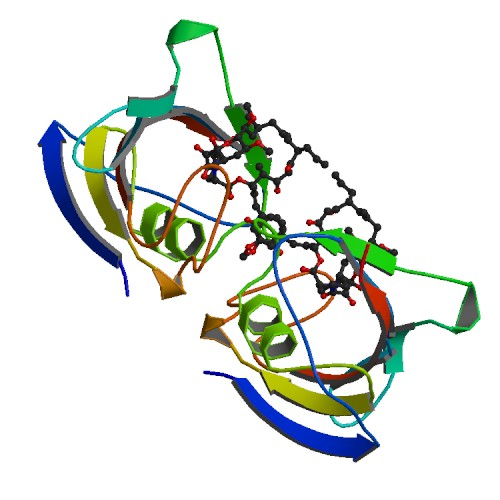
\includegraphics[width=\textwidth]{1fkj.jpg}
		\caption{1FKJ}
		\label{fig:1FKJ}
	\end{subfigure}
	~ %add desired spacing between images, e. g. ~, \quad, \qquad, \hfill etc. 
	%(or a blank line to force the subfigure onto a new line)
	\begin{subfigure}{0.4\textwidth}
		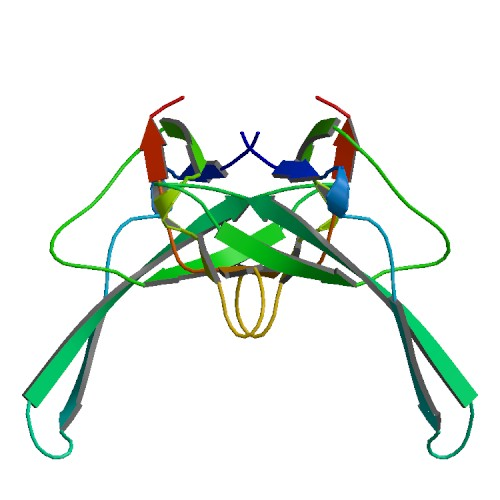
\includegraphics[width=\textwidth]{1vqb.jpg}
		\caption{1VQB}
		\label{fig:1VQB}
	\end{subfigure}
	~ %add desired spacing between images, e. g. ~, \quad, \qquad, \hfill etc. 
	%(or a blank line to force the subfigure onto a new line)
	\begin{subfigure}{0.4\textwidth}
		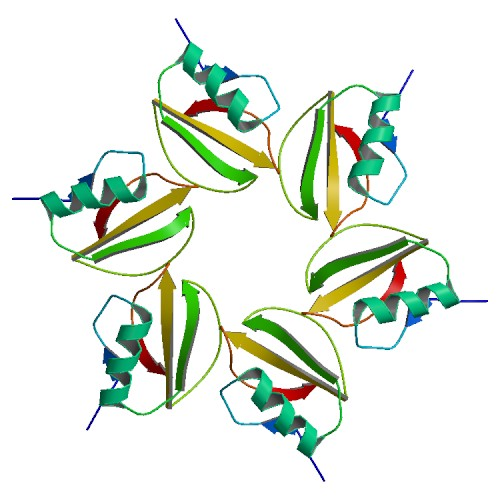
\includegraphics[width=\textwidth]{2ci2.jpg}
		\caption{2CI2}
		\label{fig:2CI2}
	\end{subfigure}
	
	\begin{subfigure}{0.4\textwidth}
		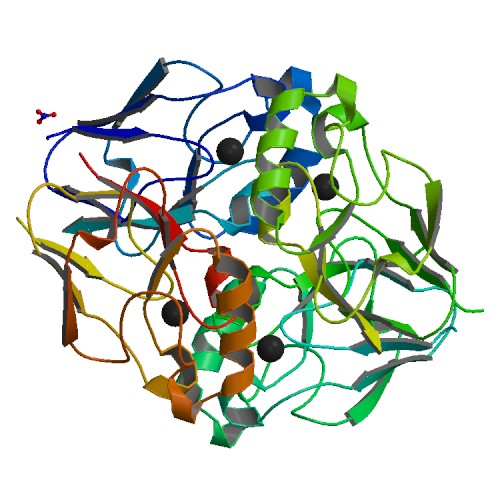
\includegraphics[width=\textwidth]{5azu.jpg}
		\caption{5AZU}
		\label{fig:5AZU}
	\end{subfigure}
	\caption{Representación de estructuras de proteínas ejemplos utilizadas para el desarrollo de meta modelos de clasificación.}
	\label{fig:proteins}
\end{figure}

Las mutaciones fueron recolectadas desde diferentes set de datos, por lo que, en caso de información ambigua, es decir, una misma mutación con diferentes respuestas, no fueron consideradas. Por otro lado, debido a que para la aplicación de la herramienta SDM se necesitaba la cadena a la cual pertenece en residuo, scripts desarrollados en Python y utilizando la librería BioPython, permitieron procesar los archivos asociados a las estructuras de las proteínas, identificadas desde el Protein Data Bank (PDB) \cite{abola1984protein}. Descartando aquellas mutaciones reportadas en las que no se encontró la cadena, obteniendo como resultante la cantidad de mutaciones reportadas para cada proteína expuestas en la Tabla \ref{cap2:tab2}.

\subsubsection{Evaluación del desbalance de clases y distribución de respuestas continuas}

El desbalance de clases se evaluó en aquellos set de datos con respuesta categórica, lo cual contempla, tres posibles casos: Neutral, Estable, No Estable, esto es debido a que todos los estudios donde se evalúan mutaciones, normalmente se analizan cambios que alteren la estabilidad de la proteína. En la Figura \ref{fig:desbalance}, se aprecia a modo ejemplo dos set datos y su distribución de categorías para la variable respuesta.

\begin{figure}[!h]
	\centering
	\begin{subfigure}{0.8\textwidth}
		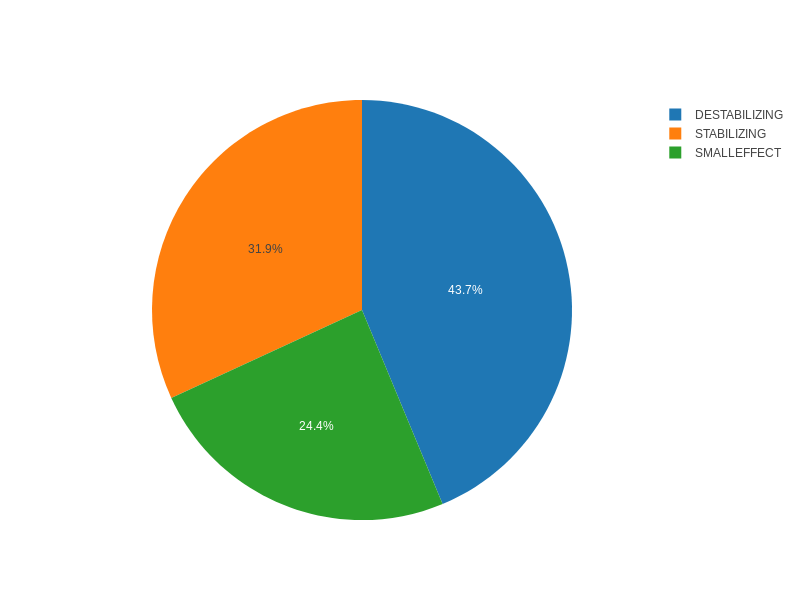
\includegraphics[width=\textwidth]{class1STN.png}
		\caption{1STN}
		\label{fig:des1}
	\end{subfigure}
	~ %add desired spacing between images, e. g. ~, \quad, \qquad, \hfill etc. 
	%(or a blank line to force the subfigure onto a new line)
	\begin{subfigure}{0.8\textwidth}
		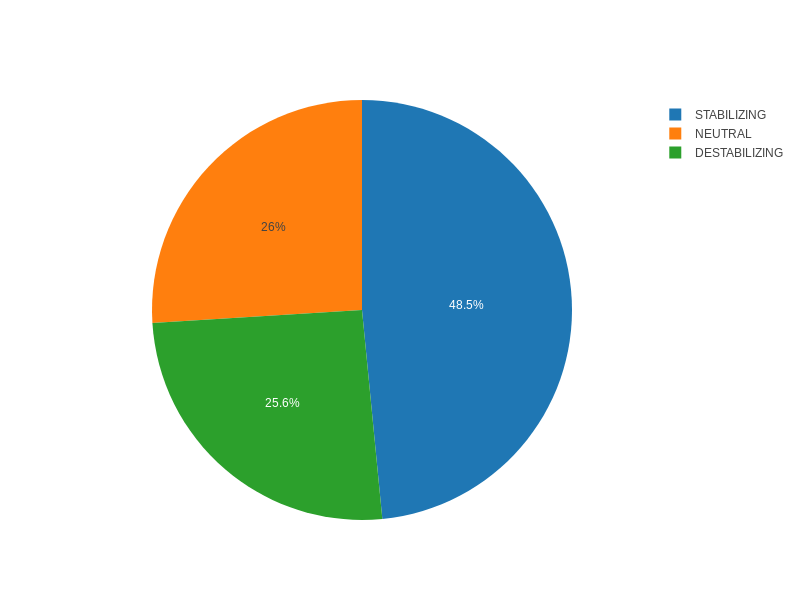
\includegraphics[width=\textwidth]{class2RN2.png}
		\caption{2RN2}
		\label{fig:des2}
	\end{subfigure}
	
	\caption{Evaluación del desbalance de clases en proteínas ejemplo.}
	\label{fig:desbalance}
\end{figure}

En las 8 proteínas en estudio para modelos de clasificación, la distribución de las categorías es similar a lo expuesta en la Figura \ref{fig:desbalance} para todas ellas, donde cerca del 50\% corresponden a mutaciones que afectan positivamente a la estabilidad, mientras que mutaciones que provocan cambios negativos o no generan diferencias, se encuentran en proporciones similares, ambas cercanas al 25\%. 

Si bien las proporciones son dispares, para este caso, se considera un desbalance como un elemento que representa menos de un 5\% del total de la muestra, además, dado a que la cantidad de ejemplos son elevadas, un 20\% o un 25\% implica cerca de 200 mutaciones, en promedio, que cumplen dicha característica. También, el hecho de que exista una cantidad inferior de mutaciones no benéficas a la estabilidad viene dada a la dificultad de encontrar y reportar mutaciones que afecten negativamente a para una proteína, es debido a la propensión filogenética \cite{Olivera-Nappa2011} que estos ocurran, lo cual se ve reflejado en las diferencias asociadas a cambios positivos dentro del set de mutaciones. No obstante, si bien el hecho de que la propensión filogenética indique que el cambio tiende a mejorar estabilidad, diseñar mutantes con mejoras en propiedades de interés, es un problema latente en la actualidad, de alto costo económico y computacional y con una gran demanda desde diferentes áreas del conocimiento.

En los set de datos para el desarrollo de modelos de regresión, se evaluó la distribución de la respuesta, en este caso, valores de $\Delta\Delta\ G$ asociado a diferencias de energía libre producidas entre el residuo mutado y el original, tal que: $\Delta\ Res_{mut}\ - \Delta\ Res_{wild}\ = \Delta\Delta\ G$. 

Las distribuciones se evaluaron utilizando el test de Shapiro, con el fin de determinar si la distribución se comportaba como una normal. Para todas las proteínas estudiadas, en los 11 set de datos, las respuestas presentaron distribución normal, con valores de Shapiro sobre 0.8 y un p-value $\leq$ 0.01, lo cual indica una alta confianza estadística en los resultados presentados por dicho test.

Una visualización de las distribuciones puede generarse a partir del desarrollo de histogramas, los cuales, a modo de ejemplo se expone en la Figura \ref{fig:histogram}.

\begin{figure}[!h]
	\centering
	\begin{subfigure}{0.48\textwidth}
		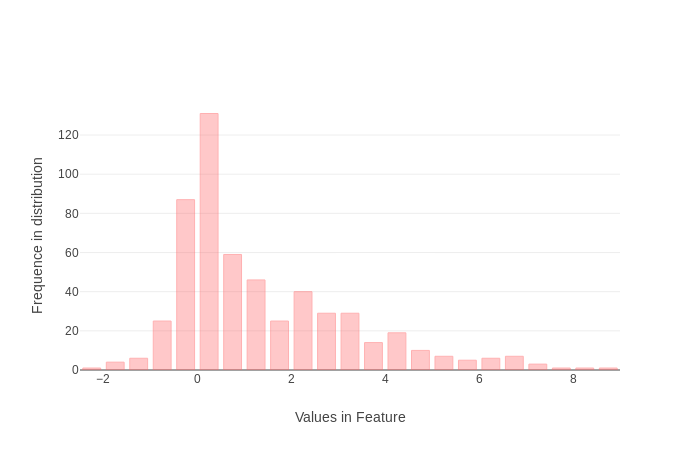
\includegraphics[width=\textwidth]{1RX4.png}
		\caption{Histograma para respuesta continua en 1RX4}
		\label{fig:hist1}
	\end{subfigure}
	~ %add desired spacing between images, e. g. ~, \quad, \qquad, \hfill etc. 
	%(or a blank line to force the subfigure onto a new line)
	\begin{subfigure}{0.48\textwidth}
		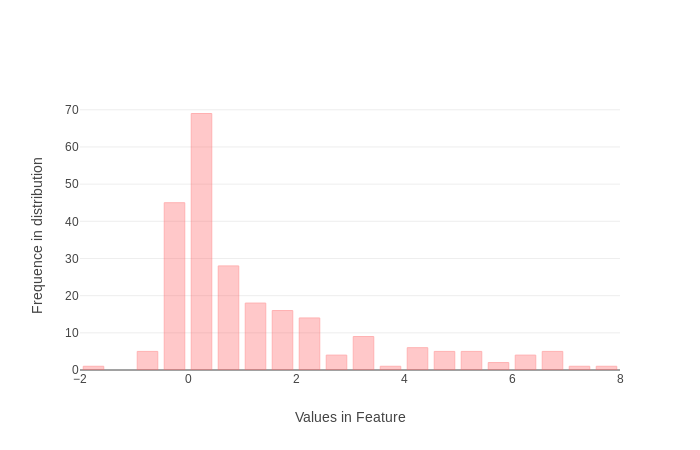
\includegraphics[width=\textwidth]{1WQ5.png}
		\caption{Histograma para respuesta continua en 1WQ5}
		\label{fig:hist2}
	\end{subfigure}
	
	\caption{Evaluación de la distribución de respuesta continua en set de datos de proteínas.}
	\label{fig:histogram}
\end{figure}

El análisis de estas características es relevante a la hora de diseñar modelos de clasificación o regresión, debido a que si existe una tendencia por una clase condiciona al clasificador a \textit{"aprender en base a la mayoría"}, por lo que puede aumentar los errores en cuanto a falsos positivos, dado a que, no se tiene la cantidad de ejemplos suficientes para una clase que permitan al modelo capturar las posibles variaciones asociadas a ésta.

Dado a los análisis de evaluación de representatividad de categorías en el set de datos y distribución de respuestas continuas, se expone que los set de datos seleccionados no presentan desbalance significativo para el caso de desarrollo de modelos de clasificación y a su vez, todas las respuestas asociadas a cambios en la energía libre para modelos de regresión, presentan distribución normal. Razón por la cual, es factible el desarrollo de modelos asociados a las respuestas presenten en los set de datos seleccionados. No obstante, sólo se ha considerado el problema del desbalance y la evaluación de distribución en la respuesta continua, una vez caracterizado los set de datos a partir de las propiedades fisicoquímicas y termodinámicas, se analizarán las características y cómo éstas condicionan la clasificación o la predicción de cambios energéticos.

%!TEX root = ../thesis.tex
%*******************************************************************************
%****************************** Third Chapter **********************************
%*******************************************************************************
\chapter{Digitalización de secuencias lineales de proteínas aplicadas al reconocimiento de patrones y modelos predictivos \label{cap3}}

% **************************** Define Graphics Path **************************
\ifpdf
    \graphicspath{{Chapter3/Figs/Raster/}{Chapter3/Figs/PDF/}{Chapter3/Figs/}}
\else
    \graphicspath{{Chapter3/Figs/Vector/}{Chapter3/Figs/}}
\fi

Desarrollar modelos predictivos basados en algoritmos de aprendizaje supervisado, o, la identificación de patrones aplicando técnicas de clustering, son tareas muy relevantes a la hora de trabajar con secuencias de proteínas, ya sea para identificar grupos con características comunes o entrenar modelos predictivos de respuestas de interés. En ambos casos, se requiere el uso de conjuntos de datos altamente informativos y con características numéricas para poder utilizar los métodos implementados en las librerías actuales \cite{pedregosa2011scikit}.

Diferentes metodologías se han implementado, para manipular las variables categóricas en set de datos y lograr su codificación numérica. Enfoques basados en adición de columnas según las categorías o simple transformación empleando representaciones en conjuntos naturales, suelen ser utilizados. No obstante, generan bastante discusión sobre las nuevas representaciones. y a su vez, el hecho de aumentar el número de columnas, conlleva a incrementar las dimensiones del conjunto de datos, provocando efectos en los desempeños de los algoritmos \cite{pedregosa2011scikit}. 

Particularmente, en secuencias de proteínas, se han utilizado las frecuencias de incidencia de los residuos para codificarlos, la cual, pese a su simplicidad, ha resultado ser efectiva en diferentes casos de uso \cite{ozbudak2014protein}. No obstante, este tipo de codificación, no permite explorar el ambiente bajo el cual se encuentran los residuos y tampoco considera el efecto de propiedades fisicoquímicas ni termodinámicas.

En diferentes estudios, los residuos se describen a partir de sus propiedades fisicoquímicas y adicional a ello, se emplea información que permite describir el ambiente del residuo a caracterizar, empleando binarizaciones para describir los residuos cercanos, ya sea por medio del uso de un rango espacial, utilizando modelos o estructuras tridimensionales en donde se representan las coordenadas espaciales de los residuos, o empleando un rango lineal en secuencias lineales de proteínas \cite{capriotti2005mutant2, capriotti2008three}.

Un enfoque basado en las propiedades fisicoquímicas en combinación con la aplicación de transformaciones de Fourier, ha permitido demostrar que ciertos residuos permiten entregar las características asociadas a la propiedad en estudio, además, facilita comprender el aporte del ambiente sobre estos y representa una forma de estudio novedosa para el uso de información de secuencias lineales. Siendo una metodología ampliamente utilizada para identificar residuos que aporten a la propiedad, por medio de la representación de señales asociadas al espacio de frecuencias \cite{veljkovic1985possible, cosic2016analysis, cadet2018application}.

A pesar de ser una metodología interesante a la hora de estudiar secuencias lineales, exhiben problemas notorios sobre la selección de las propiedades relevantes a analizar, ya que, existe un número considerablemente alto de propiedades posibles a utilizar, descritas principalmente en las base de datos AAIndex \cite{Kawashima2000}, y es factible que diferentes familias de proteínas exhiban comportamientos notoriamente no similares y diverjan en cuanto a las propiedades que puedan ser representativas, inclusive, a la hora de estudiar mutaciones en una misma proteína puede que no sólo una propiedad permita su caracterización, si no, que un conjunto pequeño de éstas \cite{cadet2018application}.

En el presente capítulo, se exponen en detalle, diferentes formas de representar secuencias lineales de proteínas, seguido a su vez del planteamiento del uso de transformadas de Fourier para la digitalización de propiedades fisicoquímicas y cómo es posible utilizar éstas para la identificación de patrones en secuencias lineales o el desarrollo de modelos de clasificación/regresión y la exposición de casos de uso en diferentes proteínas de interés. 

\section{Metodologías asociadas a la codificación de variables categóricas}

Diferentes metodologías existen para poder codificar variables categóricas, a su vez, para set de datos de proteínas con secuencias lineales, es factible utilizar sus propiedades fisicoquímicas o frecuencias de residuos. Las principales metodologías usadas a la fecha se expone a continuación.

\subsection{One Hot encoder}

One Hot encoder, es una de las técnicas más utilizadas a la hora de codificar variables categóricas y se basa principalmente en la adición de columnas con respecto a las categorías existentes en un conjunto de datos \cite{brownlee2017one}.

Dado el vector  $x$ de tamaño $n$ con $m$ categorías, por definición, One Hot encoder agrega al conjunto de datos $m$ columnas, tal que, por cada categoría se adiciona una nueva columna al set de datos. Las nuevas columnas se completan con una binarización de los elementos, indicando si el elemento $x_{i}$ posee la categoría $m_{j}$ con un valor 1 y en caso contrario 0. Es posible expresar esto como se expone a continuación.

Sea $x$ vector de $m$ categorías de dimensiones
$n \times 1$ representado por
\[ x = \left( \begin{array}{ccc}
x_{0}\\
x_{1}\\
\vdots\\
x_{n-1} \end{array} \right)\] 
Su codificación mediante One Hot Encoder corresponde al vector x'(x)
\[ x'(x) = \left( \begin{array}{ccccc}
1 & 0 & 0 & \cdots & 0 \\
0 & 1 & 0 & \cdots & 0 \\
\vdots\\
0 & 0 & 0 & \cdots & 1 \end{array} \right) \] 

Esta metodología, si bien es altamente usada, implica que, a medida que aumentan la cantidad de categorías incrementan el número de columnas a agregar en el set de datos, es decir, si se tienen $m$ categorías se adicionan $m$ columnas. Esto último, puede provocar que los set de datos se afecten por problemas relacionados con la \textit{maldición de dimensionalidad} \footnote{Ver sección \ref{problemas}}, ya que, a medida que aumentan los descriptores, aumenta la probabilidad de que estos no sean informativos, provocando una adición de información innecesaria y que perjudicaría el rendimiento de los algoritmos de aprendizajes supervisado y no supervisado.

\subsection{Ordinal encoder}

Ordinal encoder, es una simplicación de One Hot encoder, ya que, simplemente codifica las categorías con números en el conjunto $[0, m-1]$. Es decir, sea el vector $x$ de tamaño $n$ con $m$ categorías y sea $M$ el espacio de las posibles categorías con $M = [m_{1}, \cdots, m_{m}]$, y cuya codificación implica el vector $M' = [0, \cdots, m-1]$. $\forall $ elemento que $\in$ a $x$ se obtiene su codificación a partir del elemento $M'(M(m_{i}))$ que corresponde a la codificación de la categoría en el espacio $M$ \cite{pedregosa2011scikit}.

Es posible cuestionar esta metodología con respecto al orden en que trata las categorías, la representación de la información y el mantenimiento del significado de la data. Razón por la cual, se usa sólo en los casos en que la adición de múltiples descriptores empleando One Hot Encoder sea perjudicial a la hora de implementar modelos de clasificación o regresión, e inclusive, en la búsqueda de patrones.

\subsection{Frecuencias de residuos}

Una secuencia lineal de proteína, corresponde a un vector $v$ de tamaño $n$ donde cada elemento corresponde a un residuo que pertenece a la secuencia. El uso de esta información para alimentar modelos de clasificación o regresión conlleva la codificación de sus elementos. Sin embargo, a la hora de utilizar las codificaciones basadas en One Hot Encoder, el conjunto de datos no queda estándar en cuanto a sus dimensiones, ya que, el largo de las secuencias puede variar y a su vez, el número de columnas a agregar corresponde a $n \times 20$ dado a que son $n$ residuos y el espacio muestral $M$ es de tamaño 20 lo que genera un aumento considerable en la cantidad de dimensiones.

Con el fin de poder representar las secuencias lineales de proteínas, se idearon metodologías que consideran la frecuencia de aparición de los residuos en la secuencia, de tal manera, de poder codificarla en un vector de tamaño 20, donde cada elemento representa el número de incidencias del residuo dividido por el largo del vector. Así, cada elemento se encuentra en un rango $[0,1]$ donde 0 indica no incidencia del residuo y 1, incidencia total \cite{ozbudak2014protein}.

Expresado de forma matemática, sea $s$ una secuencia lineal de proteínas con $r$ residuos, su codificación se basa en la frecuencia de aparición del residuo en $s$, tal que, sea $R$ el espacio de los posibles residuos $r$ en $s$, se estima para cada $r_{j} \in\ R$ su frecuencia:

\begin{center}
	$frec(r_{j}) = \dfrac{cont(r_{j})\ if\  (r_{i}==r_{j})}{n}$
\end{center}

Finalmente, se tiene que cada residuo $r_{i}$ se representa en su valor de frecuencia $frec(r_{i})$, generando un set de datos de tamaños $s \times 20$ con $s$ secuencias representadas por un vector de tamaño 20.

Esta es una de las representaciones más utilizadas y más simples a la hora de codificar secuencias lineales de proteínas. Sin embargo, presenta diferentes problemas tales como:

\begin{itemize}
	
	\item Si los residuos se encuentran en proporciones similares, se generarán conjuntos de datos con atributos no informativos, ya que, disminuirá la varianza existente para dicho atributo, provocando una redundancia de datos.
	
	\item No considera información sobre los residuos asociados a propiedades fisicoquímicas, esto complica el hecho de representar un set de datos de secuencias o mutaciones, ya que no representa la realidad y sólo expone el comportamiento de las frecuencias de residuos, favoreciendo a aquellos con una mayor incidencia en sus elementos.
	
	\item La codificación por frecuencias es utilizada como un primer acercamiento a la representación del problema y principalmente perjudica a los modelos ya que puede generar atributos no informativos, como lo son los residuos sin incidencia, esto conlleva a modelos sobre ajustados y a creación de set de datos no informativos.
	
	\item No evalúa elementos relevantes a la caracterización de residuos claves, ambiente bajo el cual ocurren mutaciones o componentes adicionales que facilitarían una mayor comprensión del problema, ya que, sólo conocer las incidencias, proporciona un conocimiento sobre la moda y cuáles son los residuos más relevantes. No obstante, sólo permite inferir características, relacionadas a estos.
\end{itemize}

El uso de las frecuencias de residuos, es una de las primeras aproximaciones a la codificación de secuencias lineales de proteínas. No obstante, en todos los casos donde han sido utilizadas, se agrega información adicional, que permite comprender diferentes comportamientos y evalúa ciertas propiedades del entorno, razones por las cuales, se recomiendan utilizarlas en conjunto con otros descriptores. 

\subsection{Uso de propiedades fisicoquímicas}

El uso de propiedades fisicoquímicas para describir un residuo, es ampliamente empleado en la generación de descriptores para conjuntos de datos en ingeniería de proteínas \cite{capriotti2005mutant2, capriotti2008three}. Diversos enfoques y modelos han sido construidos o entrenados, contemplando información asociada a componentes termodinámicos del residuo, en particular, a la hora de describir residuos para evaluar cambios en la energía libre, relacionados a efectos en la estabilidad de una proteína \cite{ancien2018prediction, broom2017computational, 1gzp030}.

Se han reportado cerca de 570 propiedades fisicoquímicas que pueden ser utilizadas para describir un residuo en una secuencia lineal de proteínas, almanceadas en la base de datos AAIndex \cite{Kawashima2000}. A su vez, es posible caracterizar estos residuos empleando un conjunto de propiedades estructurales, termodinámicas e inclusive filogenéticas. Es decir, diferentes puntos de vista que permitan describir los residuos pertenecientes a una secuencia. Sin embargo, el hecho de seleccionar qué descriptores son relevantes y cuáles no, radica en un problema de evaluación de características, el cual es común, en el área de la minería de datos. 

Dado al gran conjunto de propiedades existentes y a la diversidad de descriptores que pueden ser utilizados para un conjunto de secuencias lineales de proteínas, es necesaria una selección correcta de las características, las cuales permitan formar set de datos informativos y con una correlación mínima entre sus elementos. 

Contemplando esta problemática, técnicas de reducción de dimensionalidad o análisis de características son las más utilizadas a la hora de seleccionar los descriptores más informativos para un conjunto de datos. No obstante, en ocasiones, el conocimiento sobre el problema es un factor relevante a considerar. 

Dada la relevancia de la selección de descriptores correctos para poder caracterizar y codificar secuencias lineales a partir de propiedades, se describen a continuación, algunas técnicas de reducción de dimensionalidad y análisis de características que pueden ser empleadas para dar solución a esta problemática.

\subsubsection{Técnicas de reducción de dimensionalidad}

Diferentes técnicas para el análisis de características y reducción de dimensionalidad han sido implementadas en el campo de minería de datos, con el fin de poder permitir la selección de descriptores informativos y sin contemplar conjuntos de datos altamente dimensionales. Dentro de las principales destacan: Análisis de correlación, mutual information, evaluaciones de características con respecto al entrenamiento de modelos empleando Random Forest, Análisis de componentes principales (PCA) y sus variantes como métodos lineales y reducción de dimensionalidad empleando métodos no lineales. 

\subsubsection{Análisis de correlación}

La correlación entre elementos, es posible definirla como una relación estadística entre dos variables aleatorias, asociado principalmente, a relacionales lineales entre ellas \cite{cohen2014applied}. Existen diferentes coeficientes de correlación, dentro de los cuales, el más conocido es Pearson. No obstante, se encuentran además: Spearman rank, kendall $\tau$. La formulación matemática de estos, fue expuesta en la sección \ref{desempeno}, en el apartado de análisis de desempeño de modelos de regresión.

De manera general, la correlación se relaciona con la covarianza entre las variables aleatorias \cite{cohen2014applied}, esto es: Sean $X$ e $Y$ variables aleatorias, el coeficiente de correlación $\rho$ entre ellas se define como:

\begin{center}
	$\rho X,Y = corr(X,Y) = \dfrac{cov(X,Y)}{\sigma_{Y}\sigma_{Y}} = \dfrac{E[(X - \mu_{X})(Y - \mu_{Y})]}{\sigma_{Y}\sigma_{Y}}$
\end{center}

$\rho \in [-1, 1]$ de tal forma que -1 indica una correlación inversa entre los elementos y 1 una relación positiva. En efectos prácticos, ambos valores denotan una dependencia entre los elementos, por lo que no son informativos y es posible eliminar uno de ellos, dada la redundancia de información. Valores cercanos a 0, indican que las variables no se encuentran correlacionadas.

Estos estudios se realizan para todas las variables en un conjunto de datos, expresándose en matrices de correlación, las cuales, pueden ser visualizadas mediante Heat Map en donde se expone la dependencia entre los atributos. Siendo una de las técnicas más utilizadas para la reducción de dimensionalidad, debido a su simpleza y a las ventajas que posee con respecto a la información que entrega sobre los atributos.

\subsubsection{Mutual information}

Es una medida de dependencia mutua entre dos variables aleatorias, permitiendo cuantificar la cantidad de información obtenida alrededor de una variable aleatoria vista desde otra. Representa un concepto más general que el análisis de correlación y se basa en la comparación de la similitud entre las distribuciones del conjunto de las variables independientes, con respecto al producto de éstas \cite{peng2005feature}.

Sean dos variables aleatorias $X$ e $Y$ con valores en el espacio $X \times Y$ y sea el conjunto $P_{(X,Y)}$ y las distribuciones marginales son $P_X$ y $P_Y$, respectivamente. El mutual information score para las variables $X$ e $Y$ es:

\begin{center}
	$I(X,Y) = D_{KL}(P_{(X,Y)} || P_X \otimes P_Y)$
\end{center}

Esto puede variar con respecto al tipo de variable a utilizar. En el caso de que pertenezcan a una distribución discreta el $I(X,Y)$ corresponde a:

\begin{center}
	$I(X,Y) = \sum_{y_{i} \in Y} \sum_{x \in X} P_{(x,y)} (x,y) \log (\dfrac{P_{(x,y)}(x,y)}{P_{x}(x)P_{y}(y)})$ 
\end{center}

Mientras que para el caso de variables con distribución continua se tiene:

\begin{center}
	$I(X,Y) = \int_{y} \int_{x} P_{(x,y)} (x,y) \log (\dfrac{P_{(x,y)}(x,y)}{P_{x}(x)P_{y}(y)})$
\end{center}

Como interpretación, se tiene que presenta un rango de valores no negativos, donde un valor 0 indica que no existe información mutua entre ambas características y a mayor valor más relación existe entre ambos elementos.

\subsubsection{Análisis espaciales de características}

En la sección \ref{rf}, se describió Random Forest como un algoritmo de aprendizaje supervisado, que permite entrenar modelos utilizando árboles de decisión para manipular las características, generando $n$ iteraciones, en donde se construyen $n$ árboles, con diferentes atributos y ejemplos. Esto, permite estabilizar las medidas de desempeño y generar modelos robustos y con probabilidades menores de sobreajuste.

Sin embargo, este método puede ser utilizado con el fin de evaluar las características, ya sea en torno a cuáles son las frecuencias con las que permite dividir de manera inicial el conjunto de datos o cuáles son las que permiten generar la clasificación o la asignación a un intervalo en términos de regresión \cite{saeys2008robust}. 

A partir de lo anterior, la profundidad de una característica utilizada como nodo de decisión en un árbol puede usarse para evaluar la importancia relativa de esa característica con respecto a la predictibilidad de la variable objetivo. Las características utilizadas en la parte superior del árbol contribuyen a la decisión de predicción final de una fracción mayor de las muestras de entrada. La fracción esperada de las muestras a las que contribuyen puede, por lo tanto, usarse como una estimación de la importancia relativa de las características \cite{granitto2006recursive}. 

La fracción de muestras a las que contribuye una característica se combina con la disminución de la impureza al dividirlas para crear una estimación normalizada del poder predictivo de esa característica \cite{saeys2008robust}.

\subsubsection{Métodos de reducción de dimensionalidad lineales}

Reducción de dimensionalidad, como su nombre lo sugiere, implica remover características o atributos del set de datos, con el objetivo de disminuir el número de dimensiones del conjunto de elementos. Esto permite descartar los atributos menos informativos o con menor relevancia, ya sea en términos de aporte a la varianza o relaciones con el resto de descriptores \cite{hinton2006reducing}.

Dentro de las principales técnicas de reducción lineales, se encuentran el Análisis de componentes principales (PCA) y sus variantes, tales como: Incremental PCA \cite{jolliffe2011principal}. 

Análisis de Componentes Principales (PCA, por sus iniciales en inglés), es una técnica estadística que permite la conversión de un conjunto de variables posiblemente correlacionadas a un conjunto de variables no correlacionadas linealmente. Estos elementos se denominan componentes principales. Su principal característica es que son ordenados de mayor a menor, según la varianza que entregan a los datos \cite{jolliffe2011principal}.

Intuitivamente, es posible pensar el PCA como un elipsoide n-dimensional de datos, donde cada eje del elipsoide representa un componente principal. Esto implica, que si algún eje del elipsoide es pequeño, la varianza correspondiente a lo largo de éste también lo es, por lo que omitir dicho eje no implica una pérdida importante de información, lo cual es denotado como la reducción de la dimensionalidad en base a los aportes a las varianzas que denotan cada componente \cite{wold1987principal}.

\paragraph{Definición\\\\}

Matemáticamente, es posible definir PCA como una transformación lineal ortogonal de los datos a un nuevo sistema de coordenadas, tal que, la mayor varianza por alguna proyección de los datos pasa a situarse en la primera coordenada (llamado el primer componente principal), la segunda mayor varianza en la segunda coordenada, y así sucesivamente.

Se considera un conjunto de datos, $X$, con una media empírica 0, donde cada una de las filas  representan ejemplos y las columnas características o atributos $p$.

La transformación está definida por un set de vectores de dimensión $p$ que poseen pesos denotados por $ w_{(k)} = (w_{1},...,w_{p})_{(k)}$, los cuales para cada vector $x_{i}$ en $X$ se operan para dar un vector con los componentes principales $ t_{(i)} = (t_{1},...,t_{k})_{(i)}$ el cual viene dado por $ t_{k(i)} = x_{i}  w_{k}$

De tal manera que las variables individuales de $t$ considerado sobre el conjunto de datos, sucesivamente heredan la varianza máxima posible de $x$, con cada carga del vector $w$.

El primer componente $ w_{{1}} $ debe satisfacer las siguientes características:

\begin{itemize}
	
	\item $w_{1} = \arg \max_{||w||=1} \{\sum_{i}(t_{(1)})^{2}_{i}\} = \arg \max_{||w||=1} \{\sum_{i}(x_{(i)}*w)^{2}\}$
	
	\item $w_{1} = \arg \max_{||w||=1} \{||Xw||^{2}\} = \arg \max_{||w||=1} \{w^{T}X^{T}Xw\}$
	
	\item $w_{1} = \arg \max \{\frac{w^{T}X^{T}Xw}{w^{T}w}\}$
	
\end{itemize}

Los \textit{k} restantes componentes son encontrados efectuando la extracción de los primeros \textit{k-1} componentes principales desde $x$:

\begin{center}
	$\hat{x}_{k} = x - \sum_{\delta=1}^{k-1}Xw_{(\delta)}w^{T}_{(\delta)}$
\end{center}

A su vez, para encontrar el vector de carga, es necesario extraer la varianza máxima del nuevo set de datos, tal que:

\begin{center}
	$w_{(k)} = \arg \max_{||w||=1} \{||\hat{x}_{k}w||^{2}\} = \arg \max \{\frac{w^{T}X^{T}\hat{X}^{T}_{k}\hat{x}_{k}w}{w^{T}w}\}$
\end{center}

La matriz de covarianza juega un rol fundamental en este análisis, cuyo valor entre dos componentes principales viene dado por:
\begin{center}
	$Q(PC_{j}, PC_{k}) \infty (Xw_{(j)})^{T} * (Xw_{(k)})$\\
	$Q(PC_{j}, PC_{k}) = w_{(j)}^{T}X^{T}Xw_{(k)}$\\
	$Q(PC_{j}, PC_{k}) = w_{(j)}^{T}\lambda_{(k)}w_{(k)}$\\
	$Q(PC_{j}, PC_{k}) = \lambda_{(k)}w_{(j)}^{T}w_{(k)}$	
\end{center}


La principal característica que define al PCA es que es una técnica comúnmente utilizada para la reducción de la dimensionalidad, esto viene dado por la transformación que se genera, $ T = xw $ donde cada vector $ x_{(i)} $ existente en un espacio de coordenadas de variables $p$, es representado por un nuevo espacio, en el cual las variables no se encuentran correlacionadas. Sin embargo, si se utilizan $ L $ componentes principales para así utilizar los primeros $ L $ vectores de carga se obtiene una transformación truncada $ T_{L} = XW_{L} $, de tal manera que la matriz $ T_{L} $ posee los $n$ ejemplos originales. 

No obstante, sólo posee $ L $ características que definen el set de datos, de tal manera que dicha transformación es posible expresarla como:

$ t = W^{T}x$, donde $ x \in R^{p}, t \in R^{L}$, para las cuales las columnas $ p \times L $ de la matriz $ W $ forman una base ortogonal de las $ L $ características, de esta manera, al basarse en la construcción con sólo $ L $ columnas se maximiza la varianza original de los datos y se minimiza el error cuadrático tal que: 

\begin{center}
	$|| TW^{T} - T_{L}W_{L}^{T}||^{2}_{2} = ||X - X_{L}||_{2}^{2}$
\end{center}

Normalmente esta reducción es usada para el manejo de set de datos de alta dimensionalidad.

PCA presenta algunas variaciones en sus definiciones o en el uso de los datos, tales como: Incremental PCA. Este método, representa una ventaja computacional en cuanto al coste de memoria y a la manipulación de set de datos altamente dimensionales \cite{artac2002incremental}.


\subsubsection{Métodos de reducción de dimensionalidad no lineales}


\subsection{Codificación de residuos con adición de información de su entorno}

Adicional a las técnicas explicadas previamente con respecto a las codificaciones existentes, en algunos casos, no sólo basta con una única codificación del residuo, si no, que es relevante adicionar información que puede ser importante para describir los residuos. Normalmente, junto con las codificaciones basadas en propiedades fisicoquímicas, se emplean técnicas que permitan describir el ambiente bajo el cual se encuentre el residuo \cite{masso2008accurate}.

En la gran mayoría de los casos, se adiciona información de los residuos cercanos al residuo de interés, esto depende del tipo de datos bajo el cual se esté trabajando, es decir, si son secuencias lineales o son estructuras de proteínas en formato PDB \cite{capriotti2008three, capriotti2005mutant2}. 

Para el caso de que sean secuencias lineales, sea $s$ secuencia de residuos de tamaño $n$ y sea $r_{i}$ el residuo de interés a evaluar su ambiente. Se crea una ventana de tamaño $n'$ que contempla la cantidad de residuos $r_j$ cercanos al residuo $r_{i}$, de tal manera que se crea un nuevo sub conjunto $s'$ de datos de tamaño $2n'$ con $n'$ residuos a la izquierda y $n'$ a la derecha. El cual normalmente es codificado empleando binarización de elementos, así, en algunas ocasiones, a cada residuo, se le adicionan 20 descriptores que permiten indicar la ausencia o presencia de residuos cercanos a su entorno y el cual se completa con el conjunto de residuos $s'$ \cite{capriotti2008three}.

Cuando se manejan estructuras de proteínas en formato PDB, la codificación y la evaluación del ambiente es similar. Sin embargo, en vez de utilizar una ventana de tamaño $n'$ se utiliza un radio espacial de valor $x$ para el cual, se toma el residuo y se estiman las distancias de los elementos cercanos, ya sea entorno a los carbonos $\alpha$ o a otros elementos. Esto, a diferencia de las secuencias lineales, permite adicionar información sobre las propiedades de distancia, ángulos y conformación de estabilidad por interacciones electrostáticas débiles que pueden generarse a partir de la proximidad de los elementos. No obstante, es una inferencia de su uso y se requieren de diferentes tipos de elementos que permitan caracterizar los eventos asociados al ambiente estructural asociado al residuo \cite{capriotti2008three}.

Actualmente, el uso de codificaciones mediante propiedades fisicoquímicas y el empleo de información adicional basada en descriptores de ambientes, es una de las metodologías más utilizadas a la hora de generar set de datos relacionados a mutaciones. Sin embargo, debido a que sólo se considera distancia, la binarización de los elementos no se ve afectada por sustituciones en residuos lejanos al lugar de ocurrencia, lo que denota la necesidad de idear metodologías que permitan contemplar el aporte completo de residuos a la caracterización de propiedades y cómo sustituciones puntuales afectan enormemente a residuos de interés. Una de las formas en las que se ha intentado dar solución a esta problemática, es modelar las propiedades fisicoquímicas de los residuos de las secuencias, a partir del uso de transformaciones de Fourier y en particular, empleando algoritmos relacionados a dichos conceptos, que aprovechen las ventajas referidas a la manipulación de espacios de frecuencias por sobre elementos temporales.

\section{Transformaciones de Fourier}

\subsection{Transformada rápida de Fourier (FFT)}

\subsection{Uso de Transformadas de Fourier en digitalización de propiedades fisicoquímicas}

\section{Clustering}

Clustering se define como un método de aprendizaje no supervisado, en el cual se cuenta con un conjunto de datos que representan a una muestra y en base a ésta, se trata de obtener grupos de objetos, denominados clusters.

Los clusters deben cumplir con dos características fundamentales:

\begin{itemize}
	\item Los objetos que pertenezcan a un mismo clúster deben ser bastante homogéneos entre ellos.
	\item Entre los clústers debe existir un alto grado de heterogeneidad.
\end{itemize}

Los métodos de clustering se tratan, fundamentalmente, de resolver el siguiente problema: Dado un conjunto de $N$ individuos, caracterizados por la información de $n$ variables $X_{j}$ con $j$ entre $1,..,n$, se plantea el reto de ser capaces de agruparlos de manera que los individuos pertenecientes a un grupo (cluster), dada la información disponible, sean tan similares entre sí como sea posible, siendo los distintos grupos entre ellos tan disimilares como sea posible.

Básicamente, el análisis constará de un algoritmo de clusterización que permitirá la obtención de una o varias particiones, de acuerdo con los criterios establecidos.

\subsection{Criterios de Similitud}

Tal como se ha mencionado anteriormente, el hecho de tener elementos pertenecientes a un mismo grupo bastante similares entre ellos y divergentes entre distintos clúster, es la característica primordial a tratar, esto último radica en la importancia de las variables que componen a un elemento en particular y en los valores que tomen éstas.

Por lo tanto se debe determinar que tan similares o diferentes son los valores que tomen las variables con respecto al elemento al cual pertenece.

Para medir lo similar o disimilar que son los individuos existe una enorme cantidad de índices de similaridad y de disimilaridad o divergencia. Todos ellos tienen propiedades y utilidades distintas y habrá que ser consciente de ellas para su correcta aplicación al momento de hacer uso de una de ellas.

Los índices expuestos normalmente pueden ser clasificados tal como sigue:

\begin{enumerate}
	
	\item  Indicadores basados en la distancia, para lo cual se considera a los individuos como vectores en el espacio de las variables, en este sentido un elevado valor de la distancia entre dos individuos indicará un alto grado de disimilaridad entre ellos.
	
	\item Indicadores basados en coeficientes de correlación; la correlación permite indicar cuál es la fuerza y la dirección de una relación lineal entre dos variables. Se considera que dos variables cuantitativas están correlacionadas cuando los valores de una de ellas varían sistemáticamente con respecto a los valores de la otra, esto es: si se tiene dos variables (A y B) existe correlación si al aumentar los valores de A lo hacen también los de B y viceversa.
	
	\item Indicadores basados en tablas de datos de posesión o no de una serie de atributos, es decir, teniendo dos vectores A y B que representan a dos individuos de una población se hace una comparación de los elementos existentes en A y no en B, los elementos existentes en B y no en A además de la intersección entre ellos, es decir, los elementos existentes en A y en B. 
	
\end{enumerate}

\subsection{Algoritmos de Clustering}

Existen diversos algoritmos de clustering, cada uno con características que los diferencian, los cuales, pueden ser aplicados a diversos casos, dependiendo de las características de los datos de entrada, es decir, de la geometría de estos datos. Sin embargo, esta representación se basa principalmente en el uso de matrices, donde cada fila representa un ejemplo y cada columna el valor de un atributo o rasgo cualitativo para dicho ejemplo.

A continuación, se resumen algunos de los algoritmos de clustering más utilizados, explicando sus propiedades y sus características.

\subsubsection{\textit{k}-Means}

El algoritmo \textit{k}-Means, trata la separación de muestras en $ n $ grupos de igual varianza, minimizando el criterio conocido como inercia, lo que se traduce en la suma de los cuadrados dentro de los clúster.

La principal característica y deficiencia a la vez, es que se requiere que el número de grupos sea entregado, es decir, se debe entregar el valor de $k$, así, si se selecciona un valor de $k = 3$, serán tres grupos los que se encontrarán. 

Este algoritmo divide un set de $N$ ejemplos $X$ en $K$ particiones distintas denominadas clúster $C$, cada uno de ellos descrito por la media $\mu_{j}$ de las muestras en el clúster. Esta media es llamada centroide, por lo que en general, \textit{k}-means  elige sus centroides de tal manera que el principio de inercia sea reducido al mínimo, es decir, que la suma de los cuadrados de los integrantes de un mismo grupo sea mínima, a través de:

\begin{center}
	$\sum_{i=0}^{n} \min_{\mu_{j} \in C} (|| x_{j}-\mu_{i}||^{2})$
\end{center}

Sin embargo, el principio de inercia, o la suma de los cuadrados mínimos entre los integrantes de los clustering, puede sufrir varios inconvenientes:

\begin{itemize}
	\item Se hace la suposición de que las agrupaciones son convexas e isotrópicas, lo cual no se da siempre, razón por la que responde mal ante a clusters que posean forma alargadas o con formas irregulares.
	
	\item No es una métrica normalizada, es decir, se sabe que los valores más bajos son mejores y el cero es óptimo. Sin embargo, en espacios de muy de alta dimensionalidad, las distancias euclidianas tienden a ser infladas, lo que se conoce como  "la maldición de la dimensionalidad", razón por la cual, son utilizados algoritmos de reducción de la dimensionalidad, tal como PCA.
	
\end{itemize}

Ambos puntos, son posibles observarlos en la Figura  \ref{kerror}, en la cual se exponen, problemas con varianzas distintas, diferencias asociadas al tamaño de los clúster, anisotropía\footnote{Las variables varían en base a las direcciones en las que se examinan} de los datos, etc.

\begin{figure}[!h]
	
	\centering
	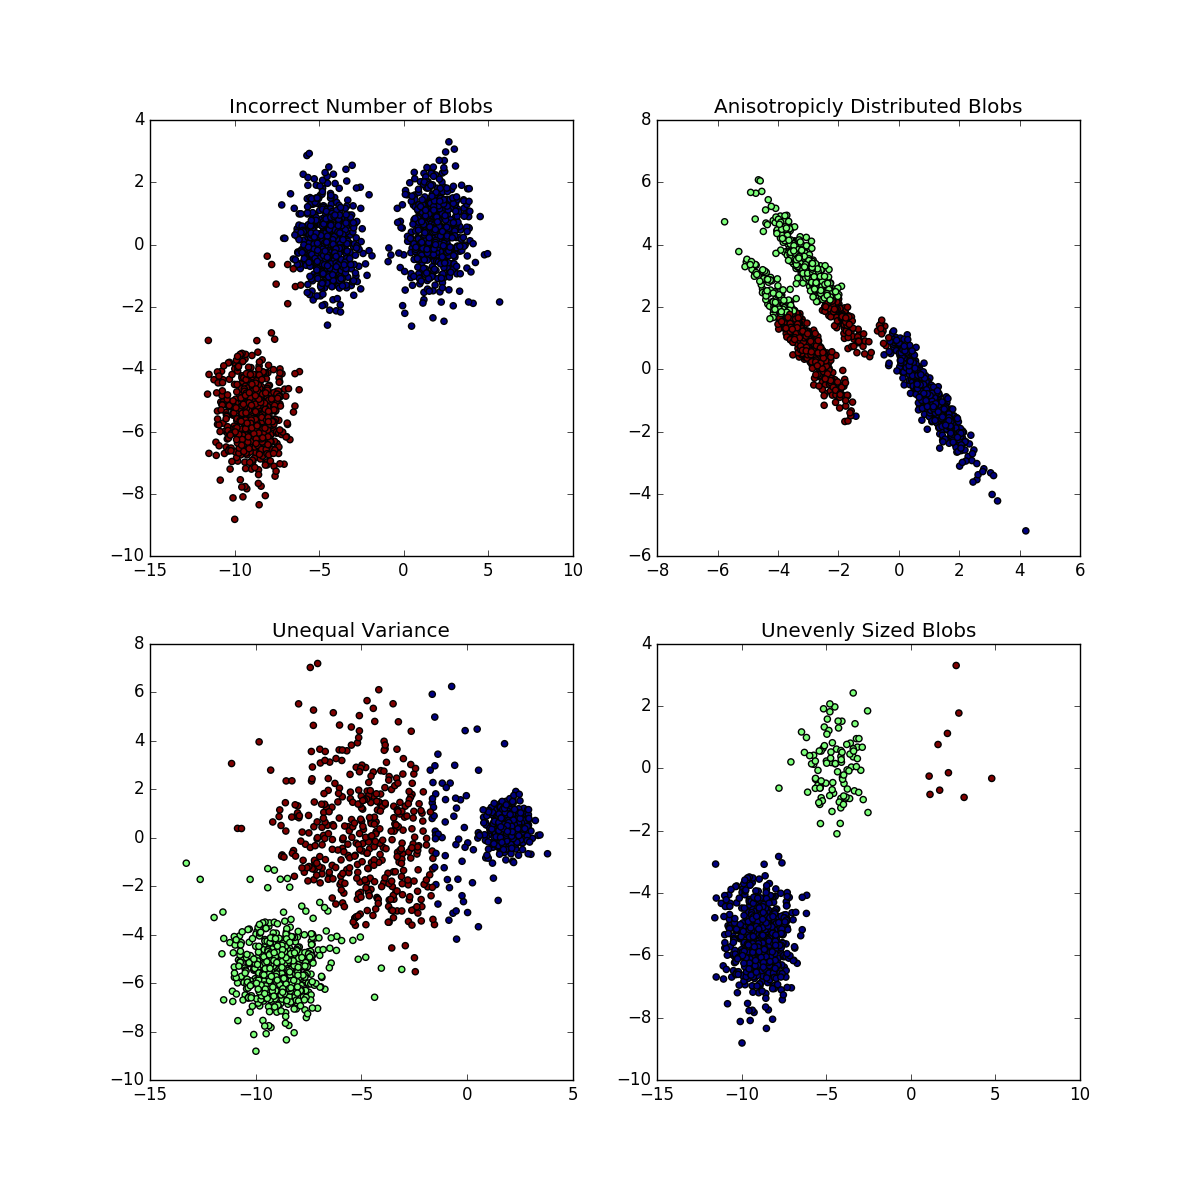
\includegraphics[scale = .4]{kmeansError.png}
	\caption{Posibles inconvenientes con los datos, donde k-medias  no funciona correctamente}
	\label{kerror}
\end{figure}


En términos básicos, el algoritmo tiene tres pasos. El primer paso consiste en elegir los centroides iniciales, con el método más básico para elegir $k$ muestras del conjunto de datos $X$. Después de la inicialización, \textit{k}-means  consta de un bucle entre los otros siguientes dos pasos. 

En una primera instancia, asigna cada muestra a su centroide más cercano. Posterior a ello, se crean nuevos centroides tomando el valor medio de todas las muestras asignadas a cada centroide anterior. La diferencia entre la media anterior y la actual (diferencia entre centroides) se calcula y se itera estas acciones hasta que este valor sea inferior a un umbral. En otras palabras, se repite hasta que los centroides no se mueven de manera significativa.

\subparagraph{Clustering Jerarquizado\\\\}

Clustering jerárquico o HCA (por sus siglas en inglés) es un método de análisis de conglomerados, que busca construir una jerarquía de agrupaciones. Las estrategias para la agrupación son posible dividirlas en dos:

\begin{itemize}
	
	\item \textbf{Aglomerativa}: consiste en un enfoque de "abajo hacia arriba": cada observación se inicia en su propio clúster, y pares de grupos se fusionan a medida que se asciende en la jerarquía. 
	
	\item \textbf{Divisiva}: consiste en un enfoque "de arriba hacia abajo": todas las observaciones se inician en un único clúster, y las divisiones se realizan de forma recursiva conforme se desciende en la jerarquía.
	
\end{itemize}

Siendo generalmente expuestos los resultados en forma de dendrograma, por otro lado, la complejidad del algoritmo, en el caso general es $\displaystyle O(n^{2}\log(n))$, lo cual presenta problemas para set de datos extensos.

Con el fin de decidir qué grupos se deben combinar (por aglomeración), o cuando un grupo se debe dividir (por división), se requiere una medida de disimilitud entre los conjuntos de observaciones. En la mayoría de los métodos de agrupación jerárquica, esto se logra mediante el uso de una métrica apropiada (una medida de la distancia entre pares de observaciones), y un criterio de vinculación que especifica la disimilitud de conjuntos como una función de las distancias por pares de observaciones en los conjuntos.

Las métricas asociadas pueden son las mismas utilizadas en el algoritmo $k$-means y las aplicadas en el método KNN de aprendizaje supervisado.


El criterio de linkage determina la distancia entre conjuntos de observaciones como una función de las distancias por pares entre observaciones.

Algunos criterios de linkage de uso común entre los dos conjuntos de observaciones $A$ y $B$ son expuestos en la tabla \ref{tab:summary-linkage}.

% Please add the following required packages to your document preamble:
% \usepackage{longtable}
% Note: It may be necessary to compile the document several times to get a multi-page table to line up properly
\begin{longtable}[c]{|l|l|}
	\hline
	\multicolumn{2}{|c|}{\textbf{Criterios de linkage comunes en métodos HCA}} \\ \hline
	\endfirsthead
	%
	\endhead
	%
	\textbf{Complete linkage clustering} & $ \max \,\{\,d(a,b):a\in A,\,b\in B\,\}.$ \\ \hline
	\textbf{Single-linkage clustering} & $ \min \,\{\,d(a,b):a\in A,\,b\in B\,\}.$ \\ \hline
	\textbf{Average linkage clustering} & $ {\frac {1}{||A||B||}}\sum _{{a\in A}}\sum _{{b\in B}}d(a,b).$ \\ \hline
	\textbf{Centroid linkage clustering} & ${\displaystyle \|c_{s}-c_{t}\|}$ con ${\displaystyle c_{s}}$ y $c_{t}$ centroides \\ \hline
	\textbf{Minimum energy clustering} & $ {\frac {2}{nm}}\sum _{{i,j=1}}^{{n,m}}\|a_{i}-b_{j}\|_{2}-{\frac {1}{n^{2}}}\sum _{{i,j=1}}^{{n}}\|a_{i}-a_{j}\|_{2}-{\frac {1}{m^{2}}}\sum _{{i,j=1}}^{{m}}\|b_{i}-b_{j}\|_{2}.$ \\ \hline
	\caption{Resumen de linkages comunes utilizados en métodos de clustering jerárquicos.}
	\label{tab:summary-linkage}\\
\end{longtable}

Un aspecto interesante de este algoritmo es que pueden ser añadidas las limitaciones de conectividad, es decir, sólo grupos adyacentes pueden fusionarse entre sí, esto es, a través de una matriz de conectividad que define para cada muestra, las muestras de vecinos después de una estructura dada de los datos. Estas restricciones son útiles para imponer una cierta estructura local, así como para hacer que el algoritmo sea más rápido, especialmente cuando el número de las muestras es alta.

\subsubsection{Affinity Propagation}

AffinityPropagation crea grupos mediante el envío de mensajes entre pares de muestras hasta la convergencia. Un conjunto de datos es descrito por el uso de un pequeño número de ejemplares, que se identifican como las más representativas de otras muestras. Los mensajes enviados entre pares representan la idoneidad para una muestra a ser el ejemplo de la otra, la cual se actualiza en respuesta a los valores de otros pares. Esta actualización ocurre de forma iterativa hasta la convergencia, momento en el que se eligen los ejemplares finales, y por lo tanto se da el agrupamiento final.

Se elige el número de grupos en base a los datos proporcionados. Para este propósito, los dos parámetros importantes son la preferencia, que controla el número de ejemplares que se utilizan, y el factor de amortiguamiento.

El principal inconveniente que presenta este algoritmo viene dado por la complejidad que posee, el cual se representa por $O(N^{2}T)$, donde $N$ es el número de muestras y $T$ es el número de operaciones necesarias para converger, razón por la cual, el uso de este algoritmo es para set de datos con pequeña cantidad de ejemplos.

Con respecto a la descripción del algoritmo, es posible mencionar que los mensajes enviados a los grupos, pertenecen a dos categorías, la primera es la responsabilidad $r(i,k)$ la cual consiste en la evidencia acumulada que denota que la muestra $k$ podría ser un ejemplar para la muestra $i$. La segunda es la disponibilidad $a(i,k)$, la cual se define como la evidencia existente para que la muestra $i$ pueda escoger a la muestra $k$ para ser su ejemplar, además considera todos los valores de las otras muestras de $k$ que podrían ser ejemplares. De esta manera, los ejemplares son escogidos por las muestras si:

\begin{itemize}
	
	\item Existe una similaridad bastante alta con respecto a las muestras.
	
	\item Si es elegido por muchas muestras y resulta ser representativo de sí mismos.
\end{itemize}

En forma matemática es posible definir la responsabilidad como:

\begin{center}
	
	$r(i, k) \leftarrow s(i, k) - max [ a(i, \acute{k}) + s(i, \acute{k}) \forall \acute{k} \neq k ]$
\end{center}

Donde $s(i,k)$ es la similaridad entre las muestras $i$ y $k$. 

A su vez, la disponibilidad, es posible definirla como:

\begin{center}
	
	$a(i, k) \leftarrow min [0, r(k, k) + \sum_{\acute{i}~s.t.~\acute{i} \notin \{i, k\}}{r(\acute{i}, k)}]$
	
\end{center}

\subsubsection{Mean Shift}

El algoritmo de Mean Shift tiene como objetivo descubrir manchas (blobs) en una densidad uniforme de las muestras. Es un algoritmo basado en centroides, que funciona mediante la actualización de los candidatos para centroides para ser la media de los puntos dentro de una región determinada. Estos candidatos se filtran en una etapa de post-procesamiento para eliminar duplicados y así formar el conjunto final de centroides.

Dado un candidato $x_{i}$ para la iteración $t$, el candidato a centroide es actualizado en base a la ecuación:

\begin{center}
	
	$x_i^{t+1} = x_i^t + m(x_i^t)$
\end{center}

Donde $N (x_i)$ es la vecindad de las muestras dentro de una distancia dada alrededor $x_i$ y $m$ es el vector de desplazamiento medio, que se calcula para cada centroide que apunta hacia una región del aumento máximo en la densidad de puntos. Ésta se calcula utilizando la siguiente ecuación, en la que la actualización de manera efectiva denota a un centroide ser la media de las muestras dentro de su vecindad:

\begin{center}
	
	
	$m(x_i) = \frac{\sum_{x_j \in N(x_i)}K(x_j - x_i)x_j}{\sum_{x_j \in N(x_i)}K(x_j - x_i)}$
	
\end{center}

Algunas de las características de Mean Shift, son

\begin{itemize}
	
	\item Ajusta automáticamente el número de grupos, dependiendo de un parámetro bandwidth, el cual se asocia al tamaño de la región en la que se debe buscar los centroides. 
	
	\item No es altamente escalable, ya que requiere múltiples búsquedas de vecinos más cercanos durante la ejecución del algoritmo. 
	
	\item Garantiza convergencia, deteniendo la iteración cuando el cambio en centroides es pequeño.
		
\end{itemize}

\subsubsection{DBSCAN}

El algoritmo DBSCAN ve agrupaciones como áreas de alta densidad separadas por zonas de baja densidad. Debido a esta visión bastante genérica, las agrupaciones que se encuentran pueden ser de cualquier forma, en lugar de \textit{k}-means  que supone que los grupos tienen la forma convexa.

El componente central de DBSCAN es el concepto de muestras de núcleo, las cuales son las muestras que se encuentran en áreas de alta densidad. Por lo tanto, un clúster es un conjunto de muestras de núcleos, cada uno cerca del otro (medido por alguna medida de distancia) y un conjunto de muestras no básicas que se encuentran cerca de una muestra básica. Hay dos parámetros necesarios para el algoritmo, min samples y EPS, los cuales definen formalmente la densidad deseada.


Más formalmente, se define una muestra del núcleo como una muestra del conjunto de datos de tal manera que existe una cantidad de muestra mínimas y a su vez otras muestras dentro de una distancia de EPS, que se definen como vecinos de la muestra del núcleo. Esto dice que la muestra de núcleo se encuentra en un área densa del espacio vectorial. Un clúster es un conjunto de muestras de núcleo que se puede construir mediante la adopción de forma recursiva de una muestra básica, la búsqueda de todos sus vecinos que son muestras de la base, la búsqueda de la totalidad de sus vecinos que son muestras de núcleo, y así sucesivamente. Un cluster también tiene un conjunto de muestras no básicas, que son las muestras que son vecinos de una muestra básica de la agrupación, pero no son en sí mismos muestras de núcleos. Intuitivamente, estas muestras están al margen de un clúster.


Cualquier muestra de núcleo es parte de un clúster, por definición. Cualquier muestra que no es una muestra del núcleo, y está al menos una distanca eps de cualquier muestra del núcleo, se considera un valor atípico por el algoritmo.

Normalmente, los resultados del algoritmo, pueden representarse tal como se expone en la Figura  \ref{dbscanE}, el color indica la pertenencia al clúster, con grandes círculos que indican muestras de núcleos encontrados por el algoritmo, círculos más pequeños son muestras no básicas que todavía son parte de un clúster. Por otra parte, los valores atípicos se indican con puntos negros.

\begin{figure}[!h]
	\centering
	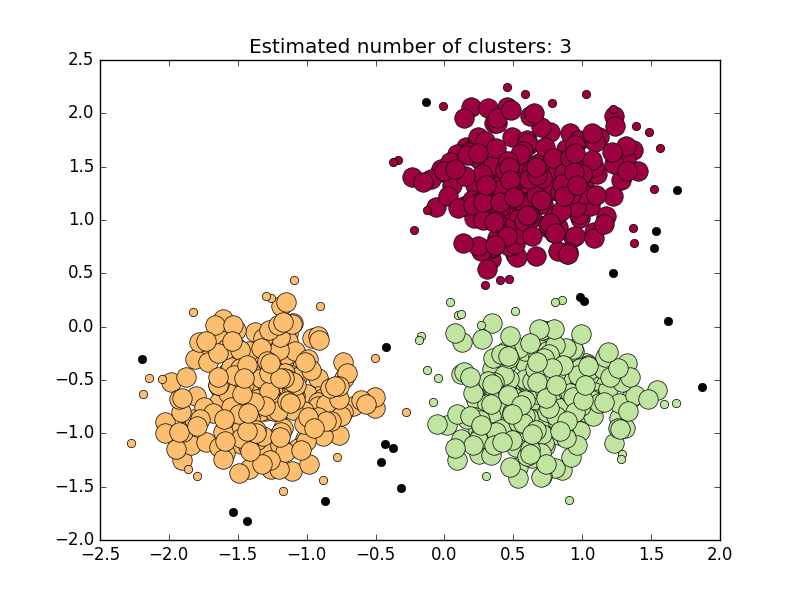
\includegraphics[scale=.4]{DBSCANexampl.png}
	\caption{Representación de resultados al aplicar la clusterización por DBSCAN}
	\label{dbscanE}
\end{figure}

\subsubsection{Birch}

Birch construye un árbol llamado Characteristic Feature Tree (CFT) de los datos correspondientes. Los datos están esencialmente con pérdida de información, comprimidos en un conjunto de nodos de rasgo característico denominados CF nodos. Estos tienen una serie de subgrupos llamados subclusters de rasgo característico, ubicados en los nodos CF no terminales los cuales pueden tener CF nodos como hijos.

Los subgrupos CF pueden contener la información necesaria para la agrupación que evite la necesidad de mantener los datos de entrada enteros en la memoria. Esta información incluye:

\begin{itemize}
	
	
	\item Número de muestras en un subgrupo.
	\item Suma lineal, representada por un vector n-dimensional que sostiene la suma de todas las muestras.
	\item Suma al cuadrado, representada por la suma cuadrática de la norma L2 de todas las muestras.
	\item Centroides, para evitar un nuevo cálculo de sumas lineales con respecto al número de muestras.
	\item Norma al cuadrado de los centroides.
	
\end{itemize}

El algoritmo de Birch tiene dos parámetros, el umbral y el factor de branching. El factor de branching limita el número de subgrupos en un nodo y el umbral limita la distancia entre la muestra de entrada y los subclusters existentes.

Este algoritmo puede ser visto como un método de instancia o reducción de datos, ya que reduce los datos de entrada a un conjunto de subclusters que se obtienen directamente de las hojas de la CFT. Estos datos reducidos pueden ser procesados por la alimentación en un clúster global. Este clúster global puede ser establecido por $n$ clusters. Si este parámetro se establece como valor 0 o ninguno, los subgrupos de las hojas se leen directamente, de lo contrario un paso global de la agrupación etiqueta estos subgrupos en grupos globales y las muestras se asignan a la etiqueta global del subgrupo más cercano.

Una descripción del algoritmo, es posible realizarla en los siguientes puntos:

\begin{itemize}
	
	\item Una nueva muestra se inserta en la raíz del árbol CF que es un nodo CF. A continuación, se fusiona con el subgrupo de la raíz, el que tiene el radio más pequeño después de la fusión, limitada por el umbral de ramificación y condiciones de los factores. Si el subcluster tiene algún nodo hijo, entonces esto se realiza repetidamente hasta que llega a una hoja. Después de encontrar el subcluster más cercano en la hoja, las propiedades de este subgrupo y los subclusters padres se actualizan de forma recursiva.
	
	\item Si el radio del subcluster obtenido mediante la fusión de la nueva muestra y el subgrupo más cercano es mayor que el cuadrado del umbral y si el número de subclusters es mayor que el factor de ramificación, a continuación, un espacio se asigna temporalmente a esta nueva muestra. Los dos subgrupos más lejanos se toman y de los subgrupos se dividen en dos grupos sobre la base de la distancia entre estos subgrupos.
	
	\item Si este nodo de división tiene un subgrupo de los padres y no hay espacio para un nuevo subgrupo, entonces el padre se divide en dos. Si no hay espacio, entonces este nodo se divide de nuevo en dos y el proceso se continúa de forma recursiva, hasta que llega a la raíz
	
\end{itemize}

\subsubsection{Mixture Model}

Los métodos de clustering basado en modelos tratan de optimizar el conjunto de datos a un modelo
matemático. En general estos métodos se basan en la suposición que los datos han sido generados por una mezcla de distribuciones de probabilidad. Dentro de los más utilizados se encuentran \textbf{Gaussian Mixture} y \textbf{Expectation-Maximization}.

Expectation Maximization, supone que los datos emergen de una mecla de distribuciones, donde cada distribución se denomina como \textit{component distribution}, razón por la cual, los datos pueden agruparse usando un modelo de mezcla de densidades de $k$ distribuciones de probabilidades. Sin embargo, el problema reside en estimar los parámetros de estas distribuciones para proveer del mejor ajuste posible a los datos. 

El algoritmo Expectation Maximization (EM) puede ser considerado como una extensión de \textit{k}-means, esto es debido a que: Si \textit{k}-means asigna cada objeto a un clúster en función de su media, EM asigna cada objeto a un clúster en función de un peso que representa la probabilidad de pertenencia al clúster. Esto requiere que se defina una distribución de probabilidad para los clusters.

Por otro lado, un modelo de mezcla gaussiano como Gaussian Mixture Model (GMM) es una función de densidad de probabilidad representada por una suma de componentes gausianas, GMMs son usadas como modelos paramétricos de la distribución de probabilidad de medidas continuas, donde los parámetros de GMM son estimados usando iterativamente el algoritmo Expectation-Maximization.

Un GMM es una suma con pesos de densidades gaussianas:

\begin{center}
	
	$p(\vec{x}) = \sum_{i=1}^{M} w_i \times N(\vec{x}|\mu_i, \sum_{i})$ 
\end{center}

Donde $\vec{x}$ es un vector D-dimensional de datos, $w_i$ son los pesos con $\sum_{i=1}^{M} w_i = 1$, y $N(\vec{x}|\mu_i, \sum_{i})$ es la densidad gaussiana, por lo tanto, la caracterización se completa con la media, la matríz de covarianza y el peso de cada componente gaussiana.

Una de las limitantes es que el número de componentes gausianos tiene que ser fijado al principio
del algoritmo.

El GMM consta de los siguientes pasos:

\begin{enumerate}
	
	\item \textbf{Iniziacilización}: para cada clase, un vector compuesto de la media y la matriz de covarianza es construido. Este vector representa las características de la distribución gaussiana usada para caracterizar las entidades del conjunto de datos. Inicialmente estos valores son generados aleatoreamente, posteriormente el algoritmo EM trata de aproximar los valores del vector de la distribución real de los datos. 
	
	\item Se estima la probabilidad de cada elemento de pertenecer a un clúster.
	
	\item Se estiman los parámetros de la distribución de probabilidad para el próximo ciclo, primero se calcula la media de la clase a través de la media de todos los puntos en función del grado de relevancia de cada punto, continuando con el cálculo de la matriz de covarianza.
	
	\item \textbf{Convergencia}: Después de cada ciclo se ejecuta un test de convergencia para verificar cuánto ha cambiado el vector de parámetros y si la diferencia es menor que un umbral de tolerancia el algoritmo se detiene, no obstante es posible detener el algoritmo debido al alcance de un número máximo de ciclos.
	
\end{enumerate}

Una representación visual del modelo es posible observarla en la Figura  \ref{esquemaR}, en ella se aprecia cómo a medida que se va iterando el algoritmo se generan los cambios y las \textit{separaciones} en grupos de clúster definidos.

\begin{figure}[!h]
	
	\centering
	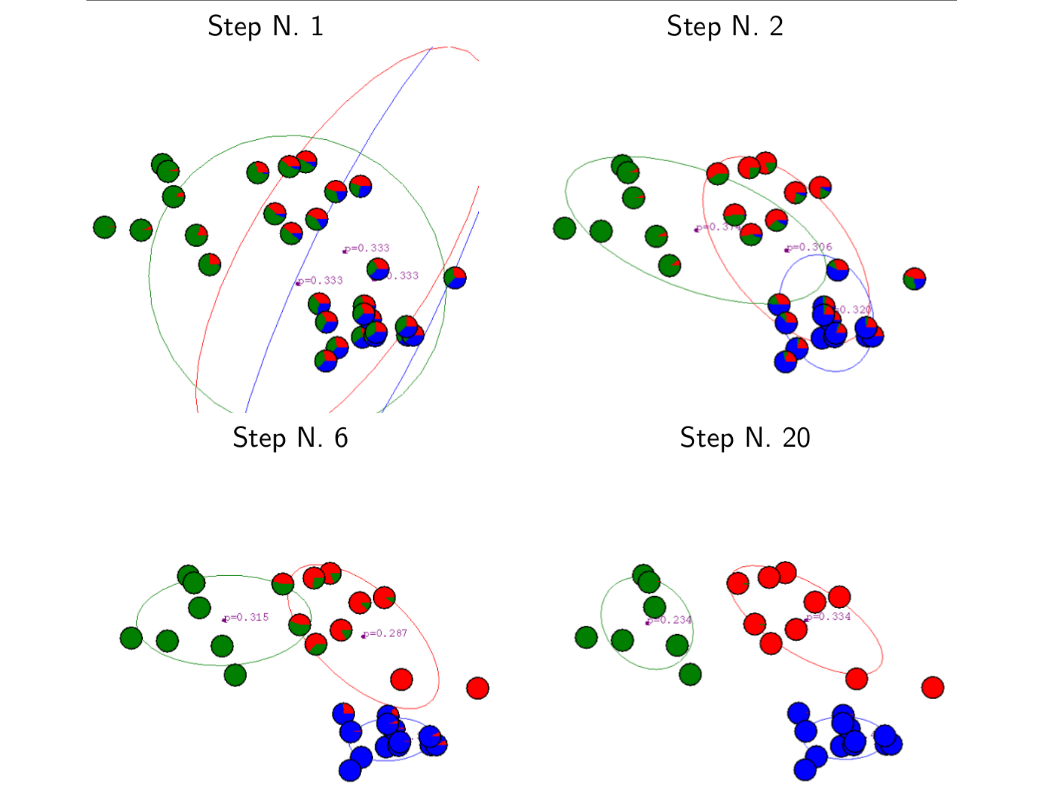
\includegraphics[scale=.4]{pasosGMM.png}
	\caption{Esquema representativo de cambios durante las iteraciones en GMM}
	\label{esquemaR}
\end{figure}

\subsubsection{Cuadro Resumen}

En la Tabla \ref{cuadroResumen} se expone un resumen de las características de cada algoritmo expuesto, la escalabilidad que poseen, las distancias que ocupan, los casos de uso y los parámetros que poseen.

\begin{table}[]
	\centering
	\begin{tabular}{|l|l|l|l|l|}
		\hline
		\multicolumn{5}{|c|}{\textbf{Tabla resumen de Algoritmos de Aprendiza No Supervisado}}                                                                                                                                                                                                                                                                                                                                                                                                                                          \\ \hline
		\textbf{Algoritmo}                                                                  & \textbf{Parámetros}                                                                       & \textbf{Escalabilidad}                                                                                  & \textbf{Usos}                                                                                                                                 & \textbf{Métrica usada}                                                              \\ \hline
		\textbf{K-Means}                                                                    & \begin{tabular}[c]{@{}l@{}}Número de \\ clúster\end{tabular}                              & \begin{tabular}[c]{@{}l@{}}Muchas muestras, \\ mediana cantidad\\ de clúster.\end{tabular}              & \begin{tabular}[c]{@{}l@{}}De propósito\\ general, la \\ geometría plana, \\ no demasiados \\ grupos\end{tabular}                             & \begin{tabular}[c]{@{}l@{}}Distancia entre\\ puntos\end{tabular}                    \\ \hline
		\textbf{\begin{tabular}[c]{@{}l@{}}Affinity \\ propagation\end{tabular}}            & preferencia                                                                               & \begin{tabular}[c]{@{}l@{}}No escalable con \\ n ejemplos\end{tabular}                                  & \begin{tabular}[c]{@{}l@{}}Muchos clúster, \\ tamañode clúster \\ desigual, \\ geometría no \\ plana\end{tabular}                             & \begin{tabular}[c]{@{}l@{}}Distancia\\ gráfica\end{tabular}                         \\ \hline
		\textbf{Mean-shift}                                                                 & bandwidth                                                                                 & \begin{tabular}[c]{@{}l@{}}No escalable con \\ n ejemplos\end{tabular}                                  & \begin{tabular}[c]{@{}l@{}}Muchos clúster, \\ tamañode clúster \\ desigual, geometría \\ no plana\end{tabular}                                & \begin{tabular}[c]{@{}l@{}}Distancia entre\\ puntos\end{tabular}                    \\ \hline
		\textbf{\begin{tabular}[c]{@{}l@{}}Ward \\ hierarchical \\ clustering\end{tabular}} & \begin{tabular}[c]{@{}l@{}}Número de \\ clúster\end{tabular}                              & \begin{tabular}[c]{@{}l@{}}Mucha cantidad \\ de ejemplos y de \\ clusters\end{tabular}                  & \begin{tabular}[c]{@{}l@{}}Cualquier clúster, \\ es posible \\ conección de \\ constraints\end{tabular}                                       & \begin{tabular}[c]{@{}l@{}}Distantia entre\\ puntos\end{tabular}                    \\ \hline
		\textbf{\begin{tabular}[c]{@{}l@{}}Agglomerative \\ clustering\end{tabular}}        & \begin{tabular}[c]{@{}l@{}}Número de \\ clúster, tipo de \\ unión, distancia\end{tabular} & \begin{tabular}[c]{@{}l@{}}Mucha cantidad\\ de ejemplos y de\\ clusters\end{tabular}                    & \begin{tabular}[c]{@{}l@{}}Muchos clusters, \\ posiblemente \\ restricciones de \\ conectividad, \\ distancias \\ no euclidianas\end{tabular} & \begin{tabular}[c]{@{}l@{}}Cualquier \\ distancia pairwise\end{tabular}             \\ \hline
		\textbf{DBSCAN}                                                                     & tamaño vecino                                                                             & \begin{tabular}[c]{@{}l@{}}Mucha cantidad \\ de ejemplos, \\ mediana\\ cantidad de clúster\end{tabular} & \begin{tabular}[c]{@{}l@{}}Geometría no plana, \\ tamaños de clusters \\ distintos\end{tabular}                                               & \begin{tabular}[c]{@{}l@{}}Distancia entre\\ puntos vecinos\end{tabular}            \\ \hline
		\textbf{\begin{tabular}[c]{@{}l@{}}Gaussian \\ mixtures\end{tabular}}               & variado                                                                                   & No escalable                                                                                            & \begin{tabular}[c]{@{}l@{}}Geometría plana, \\ bueno para la \\ estimación de la \\ densidad\end{tabular}                                     & \begin{tabular}[c]{@{}l@{}}Distancia \\ Mahalanobis para\\ los centros\end{tabular} \\ \hline
		\textbf{Birch}                                                                      & \begin{tabular}[c]{@{}l@{}}branching, \\ umbral\end{tabular}                              & \begin{tabular}[c]{@{}l@{}}Alto número de\\ clúster y ejemplos\end{tabular}                             & \begin{tabular}[c]{@{}l@{}}Largo set de datos, \\ eliminación valores \\ atípicos, \\ reducción de datos\end{tabular}                         & \begin{tabular}[c]{@{}l@{}}distancia \\ euclidiana\\ entre puntos\end{tabular}      \\ \hline
	\end{tabular}
	
	
	\caption{Cuadro resumen de algoritmos de aprendizaje supervizado}
	\label{cuadroResumen}
\end{table}

\subsubsection{Evaluación del desempeño de un clustering}\label{evaluacion}

Evaluar el desempeño de un algoritmo de clustering no es tan trivial como contar el número de errores o la precisión y la recuperación de un algoritmo de clasificación supervisada. En particular, cualquier métrica de evaluación no debe tomar los valores absolutos de las etiquetas de clúster en cuenta, sino más bien si estas agrupaciones definen separaciones de los datos, de tal manera que los miembros que pertenecen a la misma clase son más similares que los miembros de diferentes clases de acuerdo con alguna similitud métrica.

Existen diversas medidas de similitud con el fin de evaluar el clustering, las cuales se explican a continuación:

\subparagraph{Índice Rand ajustado (Adjusted Rand index)\\\\}

Dado el conocimiento de las clases asignadas como verdaderas (etiquetas verdaderas) y las etiquetas obtenidas por el algoritmo de clustering (etiquetas predichas) el adjuster rand index es una función que mide la similaridad de las dos asignaciones, ignorando permutaciones, posee valores entre -1 y 1, siendo 1 el valor perfecto. Sin embargo, es imperante para evaluar el desempeño, conocer las etiquetas verdaderas de los datos.

Matemáticamente es posible definirlo como:

Sea $C$ una asignación de clase real y dada la agrupación $K$, se define $a$ y $b$ como:

\begin{itemize}
	
	\item $a$, el número de pares de elementos que estan en el mismo set en $C$ y en el mismo set en $K$.
	\item $b$, el número de pares de elementos que estan en diferentes set en $C$ y en diferentes set en $K$.
\end{itemize}

El valor del rand index no ajustado viene dado por:

\begin{center}
	$RI = \frac{a + b}{C_2^{n_{samples}}}$
\end{center}

Donde $C_2^{n_{samples}}$ es el número total de posibles pares en el set de datos.

Sin embargo, la puntuación de RI no garantiza que las asignaciones de etiquetas al azar conseguirán un valor cercano a cero, para contrarrestar este efecto se puede descartar la esperanza RI $E[RI]$ de etiquetas al azar mediante la definición del adjusted rand index:

\begin{center}
	$ARI = \frac{RI - E[RI]}{\max(RI) - E[RI]}$
	
\end{center}

\subparagraph{Información mutua basada en scores\\\\}

Dado el conocimiento de las etiquetas de las clases reales y las asignaciones obtenidas de algoritmos de agrupación de las mismas muestras, el mutual information es una función que mide el \textit{acuerdo} de las dos asignaciones, ignorando las permutaciones. Existen dos versiones normalizadas diferentes de esta medida:

Normalized Mutual Information, NMI (Información mutua normalizada) y Adjusted Mutual Information, AMI (Información mutua ajustada). NMI es a menudo usado en la literatura mientras que AMI fue porpuesto más recientemente.

Matemáticamente, es posible definir esta forma de evaluación tal que: se asume dos etiquetas asignadas (de los mismos $N$ objetos), $U$ y $V$, su entropía es la cantidad de incertidumbre para un conjunto de particiones definido por:

\begin{center}
	$H(U) = \sum_{i=1}^{|U|}P(i)\log(P(i))$
\end{center}

donde $P(i) = |U_i| / N$ es la probabilidad que un objecto seleccionado aleatoriamente de la clase $U$ sea asignado a la clase $U_i$, de igual manera para $V$:
\begin{center}
	
	$H(V) = \sum_{j=1}^{|V|}P'(j)\log(P'(j))$
\end{center}

Con $P'(j) = |V_j| / N$ el mutual information (MI) entre $U$ y $V$ es calculado por:

\begin{center}
	
	$MI(U, V) = \sum_{i=1}^{|U|}\sum_{j=1}^{|V|}P(i, j)\log(\frac{P(i,j)}{P(i)P'(j)})$
\end{center}

donde $P(i, j) = |U_i \cap V_j| /N$ es la probabilidad de que un objeto seleccionado aleatoriamente sea asignado a ambas clases $U_i$ y $V_j$.

El valor normalizado del mutual information es definido como:

\begin{center}
	
	$NMI(U, V) = \frac{MI(U, V)}{\sqrt{H(U)H(V)}}$
	
\end{center}
Este valor del mutual information y también la variante normalizada no se ajusta al azar y tiende a aumentar a medida que aumenta el número de diferentes etiquetas (clusters), independientemente de la cantidad real de \textit{mutual information} entre las asignaciones de etiquetas.

El valor esperado para el mutual information puede ser calculado usando la ecuación descrita por  Vinh, Epps, and Bailey, (2009). En esta ecuación, $a_i = |U_i|$ (el número de elementos en $U_i$) y $b_j = |V_j|$ (el número de elementos en $V_j$).
\begin{center}
	
	$E[MI(U,V)]=\sum_{i=1}^|U| \sum_{j=1}^|V| \sum_{n_{ij}=(a_i+b_j-N)^+ }^{\min(a_i, b_j)} \frac{n_{ij}}{N}\log ( \frac{ N.n_{ij}}{a_i b_j}) \frac{a_i!b_j!(N-a_i)!(N-b_j)!}{N!n_{ij}!(a_i-n_{ij})!(b_j-n_{ij})! (N-a_i-b_j+n_{ij})!}
	$
\end{center}

Usando el valor esperado, el adjusted mutual information puede ser calculado usando una forma similar al ARI:

\begin{center}
	
	$AMI = \frac{MI - E[MI]}{\max(H(U), H(V)) - E[MI]}$
\end{center}
\subparagraph{Homogeneidad, Completación y medida V (V-measure) \\\\}

Para el caso en el que se conozca a ciencia cierta las etiquetas reales de las clases, es posible definir medidas de evaluación basándose en la entropía existente. En particular Rosenberg y Hirschberg (2007) \cite{sesentaiocho} definen los siguientes dos objetivos deseables para cualquier asignación de clusters:

\begin{itemize}
	
	\item \textbf{homogeneidad}: cada clúster contiene sólo miembros de una única clase.
	
	\item \textbf{Totalidad (completeness)}: todos los miembros de una clase son asignados a un mismo clúster.
	
\end{itemize}

Los valores de estos score abarcan los rangos entre 0 y 1, siendo 1 el score perfecto.

Es posible definir la homogeneidad y el completeness como:

\begin{center}
	
	$h = 1 - \frac{H(C|K)}{H(C)}$\\
	$c = 1 - \frac{H(K|C)}{H(K)}$
\end{center}

donde $H(C|K)$ es la entropía condicional de las clases dada la asignación del clúster y es definida por:

\begin{center}
	
	$H(C|K) = - \sum_{c=1}^{|C|} \sum_{k=1}^{|K|} \frac{n_{c,k}}{n} \cdot \log(\frac{n_{c,k}}{n_k})$
	
\end{center}

y $H(C)$ es la entropía de la clase y cuyo valor viene dado por:

\begin{center}
	
	$H(C) = - \sum_{c=1}^{|C|} \frac{n_c}{n} \cdot \log(\frac{n_c}{n})$
\end{center}

con $n$ siendo el número total de muestras, $n_c$ y $n_k$ el número de muestras respectivamente pertenecientes a la clase $c$ y al clúster $k$, y finalmente $n_{c,k}$ el número de muestra de la clase $c$ asignados al clúster $k$.

Rosenberg y Hirschberg también definieron un \textbf{V-measure} como el score medio de la homogeneidad y completeness:

\begin{center}
	
	$v = 2 \cdot \frac{h \cdot c}{h + c}$
\end{center}
\subparagraph{Coeficiente de silueta (Silhouette Coefficient)\\\\}

Este coeficiente es posible utilizarlo cuando se desconocen las reales etiquetas de los ejemplos, una puntuación alta (por sobre 0.75) denota un modelo con grupos bien definidos. Este coeficiente se define para cada muestra y posee dos score:

\begin{itemize}
	
	\item \textbf{a}: la distancia media entre un ejemplo y todos los otros puntos en la misma clase.
	
	\item \textbf{b}: la distancia media entre un ejemplo y todos los otros puntos en el siguiente clúster vecino.
\end{itemize}

El coeficiente para una única muestra, viene dado por:

\begin{center}
	
	$s = \frac{b - a}{max(a, b)}$
\end{center}


\subparagraph{ Calinski-Harabaz Index\\\\}

Este índice es utilizado cuando las etiquetas son desconocidas, donde un mayor valor de éste implica un modelo mejor definido.

Para $k$ clusters, el Calinski-Harabaz index $s$ se da como la razón de la dispersión entre clusters y la dispersión dentro del grupo:

\begin{center}
	$s(k) = \frac{Tr(B_k)}{Tr(W_k)}  \frac{N - k}{k - 1}$
\end{center}


Donde $B_{K}$ es la matriz de dispersión entre grupos y $W_{K}$ es la matriz de dispersión dentro del clúster definida por:

\begin{center}
	
	$W_k = \sum_{q=1}^k \sum_{x \in C_q} (x - c_q) (x - c_q)^T$\\
	$B_k = \sum_q n_q (c_q - c) (c_q - c)^T$
\end{center}

Con $N$ como el de puntos en el set de datos, $C_{q}$ el set de puntos en el cluster $q$, $c_{q}$ el centro del clúster $q$, $c$ el centro de $E$, $n_{q}$ el número de puntos en el clúster $q$.

\section{Hipótesis}

Dada la problemática existente sobre cómo representar conjuntos de secuencias lineales con el fin de poder desarrollar modelos de clasificación/regresión o identificación de patrones asociados a residuos claves que brindan la propiedad fisicoquímica. Y, en consideración de los diferentes usos que entrega las transformadas de Fourier, se plantea la hipótesis de este capítulo.

\begin{center}
	\textit{La codificación de secuencias lineales empleando espectros de frecuencia, basados en las propiedades fisicoquímicas de los residuos pertenecientes, permite generar descriptores que faciliten el aprendizaje de predictores de variantes enfocados a diferentes respuestas de interés? A su vez, los patrones de frecuencia, pueden ser asociados a residuos claves en familias de variantes?
}
\end{center}
Si bien, en el planteamiento de la hipótesis se exponen dos preguntas, la interrogante en sí, se centra a los posibles usos que pueda tener los espectros de frecuencia en el estudio de variantes, identificación de patrones, residuos relevantes, etc.

\section{Objetivos}

En base a la hipótesis planteada y con el fin de responder a los planteamientos e interrogantes expuestas. Se detallan el objetivo general y los objetivos específicos.

\subsection{Objetivo general}

Diseñar e implementar metodología de codificación y digitalización de propiedades fisicoquímicas en secuencias lineales de proteínas, con el fin de poder ser utilizadas en identificación de patrones por medio de técnicas de clustering o desarrollo de predictores basados en algoritmos de aprendizaje supervisado.

\subsection{Objetivos específicos}

A partir del objetivo general, nacen los siguientes objetivos específicos.

\begin{enumerate}
	
	\item Preparar y manipular base de datos de propiedades fisicoquímicas asociadas a la base de datos AAindex \cite{Kawashima2000}.
	
	\item Diseñar e implementar, metodología de codificación de propiedades fisicoquímicas y selección de las más representativas, por medio de técnicas de reducción de dimensionalidad y selección de features y descritas a través de espectros de frecuencia.
	
	\item Implementar y validar modelos de clasificación para evaluación de análisis de estabilidad de variantes según descriptores basados en espectros de frecuencia de propiedades fisicoquímicas.
	
	\item Diseñar, implementar y validar metodología para identificación de patrones asociados a residuos y la generación de clustering de espectros de frecuencia.
	
\end{enumerate}

\section{Metodología}

Con el fin de poder cumplir con el objetivo general planteado y los objetivos específicos, se expone a continuación la metodología diseñada. Se consideran diferentes etapas dentro de las cuales se destaca la codificación, entrenamiento de modelos, aplicación de clustering e identificación de residuos como patrones de señales dentro del espectro de frecuencia.

A continuación de exponen las diferentes etapas asociadas al proceso.

\subsection{Codificación de secuencias lineales}

La codificación de secuencias lineales, se basa en el uso de propiedades fisicoquímicas representativas de la secuencia, las cuales se obtienen a partir de la base de datos AAindex \cite{Kawashima2000}.

Un esquema representativo del proceso, se observa en la Figura \ref{cap3:fig1}, en la cual, se detallan los diferentes pasos a seguir para generar la codificación correspondiente y obtener los espectros de frecuencias asociados a cada propiedad fisicoquímica.

\begin{figure}[!h]
	
	\centering
	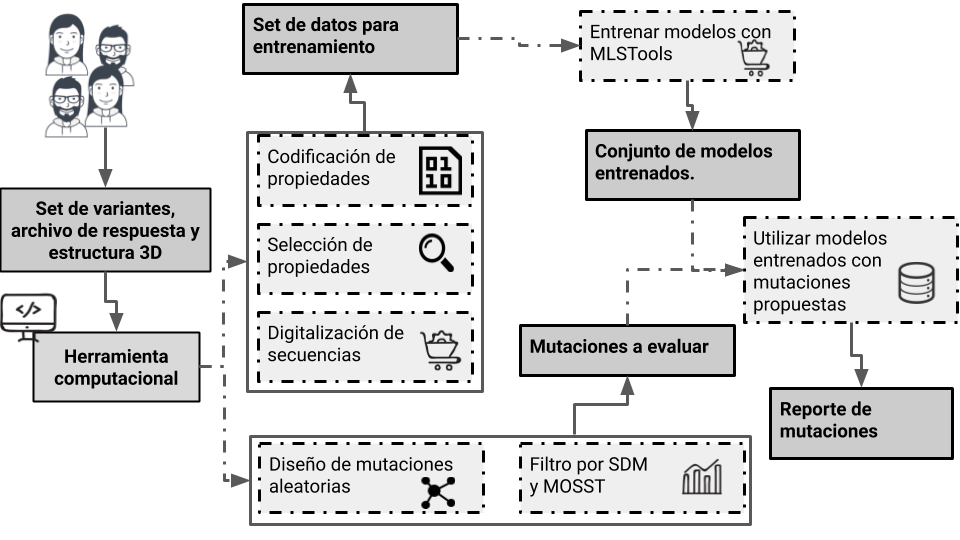
\includegraphics[scale=.4]{fig1.png}
	\caption{Esquema representativo, metodología de digitalización de secuencias.}
	\label{cap3:fig1}
\end{figure}

En una primera instancia, se toma la secuencia y por cada residuo se crea un vector de tamaño $n$ el cual representa el número de propiedades fisicoquímicas descritas en la base de datos AAindex. De esta forma, se crea una matriz de tamaño $r \times n$ donde $r$ representa la cantidad de residuos en la secuencia.


A partir de dicha matriz, técnicas de reducción de dimensionalidad y selección de características son implementadas, utilizando lenguaje de programación Python y la librería scikit-learn \cite{pedregosa2011scikit}, con el fin de seleccionar cuáles son las propiedades más representativas y qué porcentaje de la varianza permiten explicar.

Dado el conjunto de propiedades seleccionadas, se implementarán rutinas basadas en lenguaje de programación Matlab, las cuales reciben el conjunto inicial de datos, en una primera instancia, aplica "zero-padding" con el fin generar vectores de tamaño 1024, requisito para la aplicación de FFT. A partir de esto, cada columna en el conjunto de elementos, se digitaliza por medio del uso de la transformada rápida de Fourier (FFT) y se obtienen los espectros de frecuencias para cada propiedad fisicoquímica seleccionada previamente.

De esta forma, por cada secuencia, se obtiene un conjunto de espectros de frecuencia, asociados a la digitalización de las propiedades fisicoquímicas seleccionadas mediante técnicas selección de características.

\subsection{Implementación de modelos de clasificación/regresión para análisis de variantes}

Uno de los objetivos de la codificación de secuencias lineales, es evaluar si el conjunto de espectros de frecuencia para un grupo de variantes, puede ser utilizado como características para generar set de datos y entrenar modelos a partir de estos.

Con esto en mente y apoyados en los conjuntos de datos utilizados para la generación de descriptores basados en propiedades termodinámicas y filogenéticas, expuestos en el capítulo \ref{cap2}, se considerarán la secuencia original de la proteína y serán generadas las variantes con respecto a la mutación reportada. De esta forma se creará un conjunto de datos basados en una variante y la respuesta asociada, lo cual corresponde a las diferencias de energía libre que provoca la sustitución del residuo.

Al conjunto de secuencias generado, se aplicará la codificación y digitalización de las propiedades fisicoquímicas, descritas en el punto anterior. La selección de las características se basa en un consenso con respecto a las incidencias de cada propiedad en cada secuencia.

Una vez se tenga el conjunto de espectros, modelos predictivos serán entrenados aplicando algoritmos de aprendizaje supervisado al set de datos de espectros de frecuencia. Se utilizarán las medidas de desempeño expuestas en el capítulo anterior. Los modelos serán validados mediante validación cruzada con un valor de $k=10$, con el fin de evaluar el sobreajuste. 

Los modelos serán comparados con los obtenidos en la fase de exploración de la metodología expuesta en el capítulo 2 y con los resultados finales a obtener. Esto con el fin de determinar, qué metodología o caracterización de datos, permite entregar un modelo con mejor desempeño o características deseables.

\subsection{Identificación de residuos claves en espectros de frecuencia}


\subsection{Aplicación de técnicas de clustering, para categorización de espectros de frecuencia}


 
%!TEX root = ../thesis.tex
%*******************************************************************************
%****************************** Third Chapter **********************************
%*******************************************************************************
\chapter{Filogenética, propiedades fisicoquímicas y minería de datos aplicadas al diseño de mutaciones en secuencias de proteínas \label{cap4}}

% **************************** Define Graphics Path **************************
\ifpdf
    \graphicspath{{Chapter4/Figs/Raster/}{Chapter4/Figs/PDF/}{Chapter4/Figs/}}
\else
    \graphicspath{{Chapter4/Figs/Vector/}{Chapter4/Figs/}}
\fi

%!TEX root = ../thesis.tex
%*******************************************************************************
%****************************** Third Chapter **********************************
%*******************************************************************************
\chapter{Planificación y estado de avance.}

% **************************** Define Graphics Path **************************
\ifpdf
    \graphicspath{{Chapter5/Figs/Raster/}{Chapter5/Figs/PDF/}{Chapter5/Figs/}}
\else
    \graphicspath{{Chapter5/Figs/Vector/}{Chapter5/Figs/}}
\fi

Es posible pensar en este proyecto de Tesis, como un conjunto de postulaciones y planteamientos de nuevas metodologías basadas en el uso de técnicas de minería de datos que permitan estudiar mutaciones en conjuntos de datos y que culminan con una gran temática, que aborda la implementación de una herramienta computacional para el diseño de mutaciones.

Dado esto, el proyecto en sí, puede dividirse en tres grandes objetivos, de los cuales, los conocimientos y destrezas adquiridas en los primeros dos, son necesarias para cumplir con el tercer gran objetivo. Esto, es posible observarlo en la Figura \ref{cap5:fig1}.

\begin{figure}[!h]
	
	\centering
	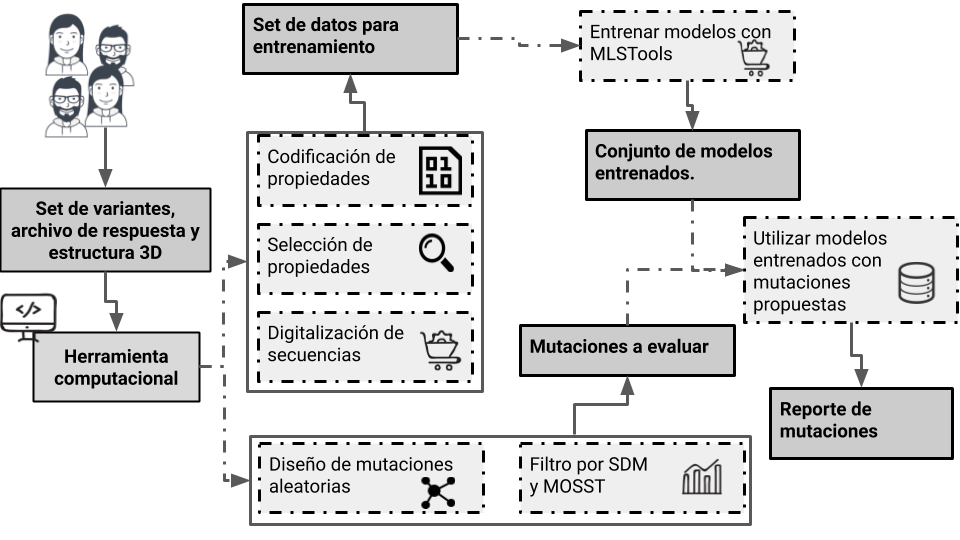
\includegraphics[scale=.5]{fig1.png}
	\caption{Esquema representativo de objetivos generales involucrados en el desarrollo del proyecto.}
	\label{cap5:fig1}
\end{figure}

El primer objetivo, se basa en la construcción de modelos de clasificación o regresión basados en algoritmos de aprendizaje supervisado, enfocados en el estudio de mutaciones puntuales en una proteína y cómo afectan éstas en términos de una respuesta conocida, como por ejemplo, estabilidad, productividad, actividad, etc. Esto, va en directo beneficio del estudio de nuevas mutantes o variantes en proteínas de interés, apoyados en una metodología que maximiza el desempeño de los modelos y sin incurrir en costos computacionales elevados. No obstante, el hecho de manipular nuevas mutaciones, requiere una verificación experimental. Sin embargo, esto permite minimizar los costos económicos y de recursos humanos que conlleva estudiar un gran conjunto de espacios muestrales de mutaciones. 

Por otro lado, el segundo objetivo se basa principalmente en representar secuencias lineales de proteínas a partir de la digitalización de propiedades fisicoquímicas y empleando transformadas de Fourier como representación de espectros de frecuencias. Si bien, el enfoque principal es la representación en sí, el objetivo también abarca el cómo utilizar estas representaciones para el entrenamiento de modelos de clasificación/regresión o el reconocimiento de patrones e identificación de residuos que aportan a las propiedades fisicoquímicas.

Finalmente, el tercer gran objetivo, comprende el desarrollo de una herramienta computacional, basada en técnicas de minería de datos para el diseño de mutaciones en proteínas de interés. El cómo se abarcará esta problemática, comprende, por un lado, definir representaciones de las secuencias lineales y cómo codificar sus propiedades fisicoquímicas, en conjunto, con el entrenamiento de modelos de clasificación/regresión que permitan evaluar nuevas mutantes. Es decir, los enfoques propuestos en los capítulos \ref{cap3} y \ref{cap2}, respectivamente. Demostrando así, las relaciones existentes entre cada capítulo y cómo estos apuntan a un objetivo general que conlleva aplicar minería de datos en el estudio de mutaciones puntuales asociados a la ingeniería de proteínas.

Con el fin de trazar los panoramas asociados al desarrollo de cada metodología y exponer el estado de avance del proyecto en cuanto a las diferentes actividades desarrolladas, en el presente capítulo, se expone un conjunto de actividades resumen de cada objetivo, asociados a un tiempo estimativo que conlleva el cumplimiento de estos y a su vez, el estado de avance actual, junto con los objetivos siguientes a tratar.

\section{Planificación}

La planificación se centra en cumplir los tres grandes objetivos y se plantea una estimación del tiempo que conlleva el desarrollo de cada una de las temáticas. Se exponen diferentes tareas generales que aportan a cumplir los objetivos y el tiempo estimativo, considerando un desarrollo general de 3 años como máximo.

\section{Estado de avance}





%!TEX root = ../thesis.tex
%*******************************************************************************
%****************************** Third Chapter **********************************
%*******************************************************************************
\chapter{Reconocimiento de patrones y extracción de información en sistemas complejos multi-dimensionales}

% **************************** Define Graphics Path **************************
\ifpdf
    \graphicspath{{Chapter6/Figs/Raster/}{Chapter6/Figs/PDF/}{Chapter6/Figs/}}
\else
    \graphicspath{{Chapter6/Figs/Vector/}{Chapter6/Figs/}}
\fi

%!TEX root = ../thesis.tex
%*******************************************************************************
%****************************** Third Chapter **********************************
%*******************************************************************************
\chapter{Un caso de estudio completo: Aplicación de técnicas de minería de datos y reconocimiento de patrones para modelar el sistema de interacción antígeno anticuerpo}

% **************************** Define Graphics Path **************************
\ifpdf
    \graphicspath{{Chapter7/Figs/Raster/}{Chapter7/Figs/PDF/}{Chapter7/Figs/}}
\else
    \graphicspath{{Chapter7/Figs/Vector/}{Chapter7/Figs/}}
\fi




% ********************************** Back Matter *******************************
% Backmatter should be commented out, if you are using appendices after References
%\backmatter

% ********************************** Bibliography ******************************
\begin{spacing}{0.9}

% To use the conventional natbib style referencing
% Bibliography style previews: http://nodonn.tipido.net/bibstyle.php
% Reference styles: http://sites.stat.psu.edu/~surajit/present/bib.htm

\bibliographystyle{apalike}
%\bibliographystyle{unsrt} % Use for unsorted references  
%\bibliographystyle{plainnat} % use this to have URLs listed in References
\cleardoublepage
\bibliography{References/references} % Path to your References.bib file


% If you would like to use BibLaTeX for your references, pass `custombib' as
% an option in the document class. The location of 'reference.bib' should be
% specified in the preamble.tex file in the custombib section.
% Comment out the lines related to natbib above and uncomment the following line.

%\printbibliography[heading=bibintoc, title={References}]


\end{spacing}

% ********************************** Appendices ********************************

\begin{appendices} % Using appendices environment for more functunality

%%!TEX root = ../thesis.tex
% ******************************* Thesis Appendix A ****************************
\chapter{How to install \LaTeX} 

\section*{Windows OS}

\subsection*{TeXLive package - full version}
\begin{enumerate}
\item	Download the TeXLive ISO (2.2GB) from\\
\href{https://www.tug.org/texlive/}{https://www.tug.org/texlive/}
\item	Download WinCDEmu (if you don't have a virtual drive) from \\
\href{http://wincdemu.sysprogs.org/download/}
{http://wincdemu.sysprogs.org/download/}
\item	To install Windows CD Emulator follow the instructions at\\
\href{http://wincdemu.sysprogs.org/tutorials/install/}
{http://wincdemu.sysprogs.org/tutorials/install/}
\item	Right click the iso and mount it using the WinCDEmu as shown in \\
\href{http://wincdemu.sysprogs.org/tutorials/mount/}{
http://wincdemu.sysprogs.org/tutorials/mount/}
\item	Open your virtual drive and run setup.pl
\end{enumerate}

or

\subsection*{Basic MikTeX - \TeX~ distribution}
\begin{enumerate}
\item	Download Basic-MiK\TeX (32bit or 64bit) from\\
\href{http://miktex.org/download}{http://miktex.org/download}
\item	Run the installer 
\item	To add a new package go to Start >> All Programs >> MikTex >> Maintenance (Admin) and choose Package Manager
\item	Select or search for packages to install
\end{enumerate}

\subsection*{TexStudio - \TeX~ editor}
\begin{enumerate}
\item	Download TexStudio from\\
\href{http://texstudio.sourceforge.net/\#downloads}
{http://texstudio.sourceforge.net/\#downloads} 
\item	Run the installer
\end{enumerate}

\section*{Mac OS X}
\subsection*{MacTeX - \TeX~ distribution}
\begin{enumerate}
\item	Download the file from\\
\href{https://www.tug.org/mactex/}{https://www.tug.org/mactex/}
\item	Extract and double click to run the installer. It does the entire configuration, sit back and relax.
\end{enumerate}

\subsection*{TexStudio - \TeX~ editor}
\begin{enumerate}
\item	Download TexStudio from\\
\href{http://texstudio.sourceforge.net/\#downloads}
{http://texstudio.sourceforge.net/\#downloads} 
\item	Extract and Start
\end{enumerate}


\section*{Unix/Linux}
\subsection*{TeXLive - \TeX~ distribution}
\subsubsection*{Getting the distribution:}
\begin{enumerate}
\item	TexLive can be downloaded from\\
\href{http://www.tug.org/texlive/acquire-netinstall.html}
{http://www.tug.org/texlive/acquire-netinstall.html}.
\item	TexLive is provided by most operating system you can use (rpm,apt-get or yum) to get TexLive distributions
\end{enumerate}

\subsubsection*{Installation}
\begin{enumerate}
\item	Mount the ISO file in the mnt directory
\begin{verbatim}
mount -t iso9660 -o ro,loop,noauto /your/texlive####.iso /mnt
\end{verbatim}

\item	Install wget on your OS (use rpm, apt-get or yum install)
\item	Run the installer script install-tl.
\begin{verbatim}
	cd /your/download/directory
	./install-tl
\end{verbatim}
\item	Enter command `i' for installation

\item	Post-Installation configuration:\\
\href{http://www.tug.org/texlive/doc/texlive-en/texlive-en.html\#x1-320003.4.1}
{http://www.tug.org/texlive/doc/texlive-en/texlive-en.html\#x1-320003.4.1} 
\item	Set the path for the directory of TexLive binaries in your .bashrc file
\end{enumerate}

\subsubsection*{For 32bit OS}
For Bourne-compatible shells such as bash, and using Intel x86 GNU/Linux and a default directory setup as an example, the file to edit might be \begin{verbatim}
edit $~/.bashrc file and add following lines
PATH=/usr/local/texlive/2011/bin/i386-linux:$PATH; 
export PATH 
MANPATH=/usr/local/texlive/2011/texmf/doc/man:$MANPATH;
export MANPATH 
INFOPATH=/usr/local/texlive/2011/texmf/doc/info:$INFOPATH;
export INFOPATH
\end{verbatim}
\subsubsection*{For 64bit OS}
\begin{verbatim}
edit $~/.bashrc file and add following lines
PATH=/usr/local/texlive/2011/bin/x86_64-linux:$PATH;
export PATH 
MANPATH=/usr/local/texlive/2011/texmf/doc/man:$MANPATH;
export MANPATH 
INFOPATH=/usr/local/texlive/2011/texmf/doc/info:$INFOPATH;
export INFOPATH

\end{verbatim}



%\subsection{Installing directly using Linux packages} 
\subsubsection*{Fedora/RedHat/CentOS:}
\begin{verbatim} 
sudo yum install texlive 
sudo yum install psutils 
\end{verbatim}


\subsubsection*{SUSE:}
\begin{verbatim}
sudo zypper install texlive
\end{verbatim}


\subsubsection*{Debian/Ubuntu:}
\begin{verbatim} 
sudo apt-get install texlive texlive-latex-extra 
sudo apt-get install psutils
\end{verbatim}

%%!TEX root = ../thesis.tex
% ******************************* Thesis Appendix B ********************************

\chapter{Installing the CUED class file}

\LaTeX.cls files can be accessed system-wide when they are placed in the
<texmf>/tex/latex directory, where <texmf> is the root directory of the user’s \TeX installation. On systems that have a local texmf tree (<texmflocal>), which
may be named ``texmf-local'' or ``localtexmf'', it may be advisable to install packages in <texmflocal>, rather than <texmf> as the contents of the former, unlike that of the latter, are preserved after the \LaTeX system is reinstalled and/or upgraded.

It is recommended that the user create a subdirectory <texmf>/tex/latex/CUED for all CUED related \LaTeX class and package files. On some \LaTeX systems, the directory look-up tables will need to be refreshed after making additions or deletions to the system files. For \TeX Live systems this is accomplished via executing ``texhash'' as root. MIK\TeX users can run ``initexmf -u'' to accomplish the same thing.

Users not willing or able to install the files system-wide can install them in their personal directories, but will then have to provide the path (full or relative) in addition to the filename when referring to them in \LaTeX.

\end{appendices}

% *************************************** Index ********************************
\printthesisindex % If index is present

\end{document}
